\documentclass[a4paper]{article}

%% Language and font encodings
\usepackage[english]{babel}
\usepackage[utf8x]{inputenc}
\usepackage[T1]{fontenc}

%% Sets page size and margins
\usepackage[a4paper,top=3cm,bottom=2cm,left=3cm,right=3cm,marginparwidth=1.75cm]{geometry}

%% Useful packages
\usepackage{listings}
\usepackage{algorithm}
\usepackage{verbatim}
\usepackage[noend]{algpseudocode}
\usepackage{float}
\usepackage{amsmath}
\usepackage{amsthm,amssymb}
\usepackage{graphicx}
%\usepackage[draft]{graphicx}
\usepackage[colorinlistoftodos]{todonotes}
\usepackage[colorlinks=true, allcolors=blue]{hyperref}

%% Operators
\newcommand{\R}{\mathbb{R}}

\lstset{
language=Matlab,                % choose the language of the code
basicstyle=\footnotesize,       % the size of the fonts that are used for the code
numbers=left,                   % where to put the line-numbers
numberstyle=\footnotesize,      % the size of the fonts that are used for the line-numbers
stepnumber=1,                   % the step between two line-numbers. If it is 1 each line will be numbered
numbersep=5pt,                  % how far the line-numbers are from the code
showspaces=false,               % show spaces adding particular underscores
showstringspaces=false,         % underline spaces within strings
showtabs=false,                 % show tabs within strings adding particular underscores
frame=single,           % adds a frame around the code
tabsize=2,          % sets default tabsize to 2 spaces
captionpos=b,           % sets the caption-position to bottom
breaklines=true,        % sets automatic line breaking
breakatwhitespace=false,    % sets if automatic breaks should only happen at whitespace
escapeinside={\%*}{*)}          % if you want to add a comment within your code
}

\title{Note - 2017 Summer Research}

\begin{document}
\maketitle

\tableofcontents

\newpage
\section{Questions}

\subsection{MMF Related}
\begin{enumerate}
\item Finding the optimal Givens rotation: 
\begin{enumerate}
\item Proposition 4 proposes to find the roots of an optimality condition derived in the supplement. However, the pMMF library appears to avoid the $A$ matrix altogether. We calculated that if we ignore $A$ then the optimal alpha should be $\arctan(b/c)/2$.
\item If this is what is being done, how do we interpret the choice in terms of optimization?
\item Why is $A$ in Proposition 4 supposed to be a diagonal matrix  
\end{enumerate}

\item In equation (10) on the multiresolution, should the second to last term be $dim(V_l),i$ instead of $dim(V_{l-1}),i$?
\item How is the clustering done?

Function called compression map in MMFmatrix.hpp
\item Algorithm 2
\begin{enumerate}

\item If $A$ is a tall, skinny matrix, how can it be reset by multiplying on left and right by a square matrix of same dimensions

\item Why is it the rows of A that are used to determine which one to eliminate? (or this is because A is always symmetric). In this case, A is referring to square matrix, not the tall skinny matrix defined in the input.
\end{enumerate}

\item Finding the optimal rotations when K>2

In Section 2.2 of second paper, ``actual rotation angle is determined by diagonalizing the Gram matrix.'' How? Maybe check the code.
\end{enumerate}

\subsection{other}
\begin{enumerate}
\item How to quantify the relationship between reduced and original Laplacian eigenvectors?
\end{enumerate}
\newpage
\section{Givens Rotations, Sparse QR - May 26}

\subsection{A $2\times 2$ Review}
\begin{itemize}
\item A 2-by-2 orthogonal matrix Q is a \textbf{rotation} if it has the form 
\[
Q = \begin{bmatrix}
    \cos\theta & \sin\theta \\
    -\sin\theta & \cos\theta
\end{bmatrix}\]
For $x \in \R^2$, $Q^Tx$ rotates $x$ counterclockwise through $\theta$.

\item A 2-by-2 orthogonal reflection matrix Q is a \textbf{reflection} if it has the form 
\[
Q = \begin{bmatrix}
    \cos\theta & \sin\theta \\
    \sin\theta & -\cos\theta
\end{bmatrix}\]

For $x \in \R^2$, $Q^Tx = Qx$ reflects $x$ with respect to 
$$\text{span}\left \{\begin{bmatrix}
    \cos\theta/2 \\
    \sin\theta/2
\end{bmatrix}\right \}$$
\end{itemize}

\subsection{General Givens Rotations}
\begin{itemize}
\item Givens rotations are used to selectively zero elements of a matrix
\item Rank 2 corrections to the identity
\item For $c= \cos\theta$ and $s = \sin\theta$,
\[G(i,k, \theta) = \begin{bmatrix}
1 &          &    &   &      &   \\
  &  \ddots  &    &   &      &   \\
  &          & c  & s &      &   \\
  &          & -s & c &      &   \\
  &          &    &   &\ddots&   \\
  &          &    &   &      & 1 
\end{bmatrix}\] 

$G$ rotates $x\in \R^n$ through $\theta$ in $(i,k)$ coordinate plane.
\item The rotation $G(i,k,\theta)^{T} \cdot A$ only affects the $i^{th}$ and $k^{th}$ rows/columns of matrix $A$.
\end{itemize}

\subsection{Sparse QR using Givens Rotation}

Given a matrix $A$, the QR factorization is unique. In $Q$, some of the columns have to span a particular subspace and the remaining columns have to form an orthogonal basis for the complement to this subspace. Thus, the orthogonal matrix cannot be sparse. Sparse QR method represents $Q$ as a product of Givens rotations, which are extremely sparse/structured matrices.(\url{https://mathoverflow.net/questions/94198/sparsity-of-qr-decomposition})

\subsection{Sparse QR Challenge}

\begin{itemize}
\item Given a sparse matrix $A \in \mathbb{R}^{m \times n}$, determine a permutation $p$ of $[n]$ such that, if $P = I_n(:,p)$, then the $R$-factor in the thin $QR$-factorization $AP^{T} = QR$ is close to being optimally sparse.
\item Use orthogonal transformations to determine $R$ from $AP^{T}$.
\item Reduces the problem $Ax = b$ down to $R^{T}RPx = PA^{T}b$, which is easier computationally when $R$ is optimally sparse. Additionally, we now no longer have to compute $Q$.
\end{itemize}

\section{pMMF}
\subsection{Wavelet Transform - June 5-7}

Given a symmetric matrix $A \in \R^{n\times n}$, a $L$ level pMMF factorization will result in 

$$H = P_{L+1} (\overline{Q}_L P_L) \cdots (\overline{Q}_2 P_2) (\overline{Q}_1 P_1) A (P_1^{T} \overline{Q}_1^{T}) (P_2^{T} \overline{Q}_2^T) \cdots (P_{L} \overline{Q}_L^{T}) P_{L+1}^T$$
Denote $Q_L = \overline{Q}_L P_L$ and we get

$$H = P_{L+1} Q_L \cdots Q_2 Q_1 A Q_1^T Q_2^T \cdots Q_L^T P_{L+1}^T$$
Notice that $(P_{L+1} Q_L \cdots Q_2 Q_1)^T$ forms the dictionary for level $L$. The first dim$(V_L)$ columns are scaling functions and the rest of its columns are wavelets. The dictionary has the form of:
\[\begin{bmatrix}
& \vline & & \vline & & \vline & & \vline  \\
& \vline & & \vline & & \vline & & \vline \\
V_L & \vline & W_L & \vline & W_{L-1} & \vline & \cdots & \vline & W_1  \\
& \vline & & \vline & & \vline & & \vline \\
& \vline & & \vline & & \vline & & \vline \\
\end{bmatrix}\]
where $V_L$ denotes the scaling functions at level $L$ and each $W_i$ denotes the wavelet functions at level $i$.

\smallskip
The scaling and  wavelet functions have the following properties:
\begin{enumerate}
\item Scaling functions and wavelets are orthonormal. That is, the dictionary is an orthonormal matrix.
\item Scaling and wavelet functions are localized in both vertex and frequency domain.
\item Wavelets centered at the very first nodes eliminated have highest frequencies - these are the wavelet functions which make up $W_1$.
\item Last vertices remaining are the centers of the scaling functions in $V_L$.
\item span($V_i$) = span($V_{i+1} \oplus W_{i+1}$)
\end{enumerate}
\smallskip
In our code, $P_n$ is split into two separate permutations -- $C_n$, which occurs when the rows and columns are clustered, and $A_n$, which occurs when we group the remaining active columns together. However, for a given $\overline{A}_n$, the grouping of active columns and the clustering take place in successive iterations of a loop. So, for each $\overline{Q}_n$, we must undo the permutations $C_{n+1}$ and $A_n$. The only exception is $n = 1$ -- in this case, we only undo $C_1$ since the active columns have not yet been grouped together. So, our dictionary ($W$) is $$W = A_n\overline{Q}_nC_nA_{n-1}\cdots\overline{Q}_2C_2A_1\overline{Q}_1C_1$$

\subsubsection{Example 1: $16 \times 16$ Community Graph}

\begin{figure}[h]
\centering
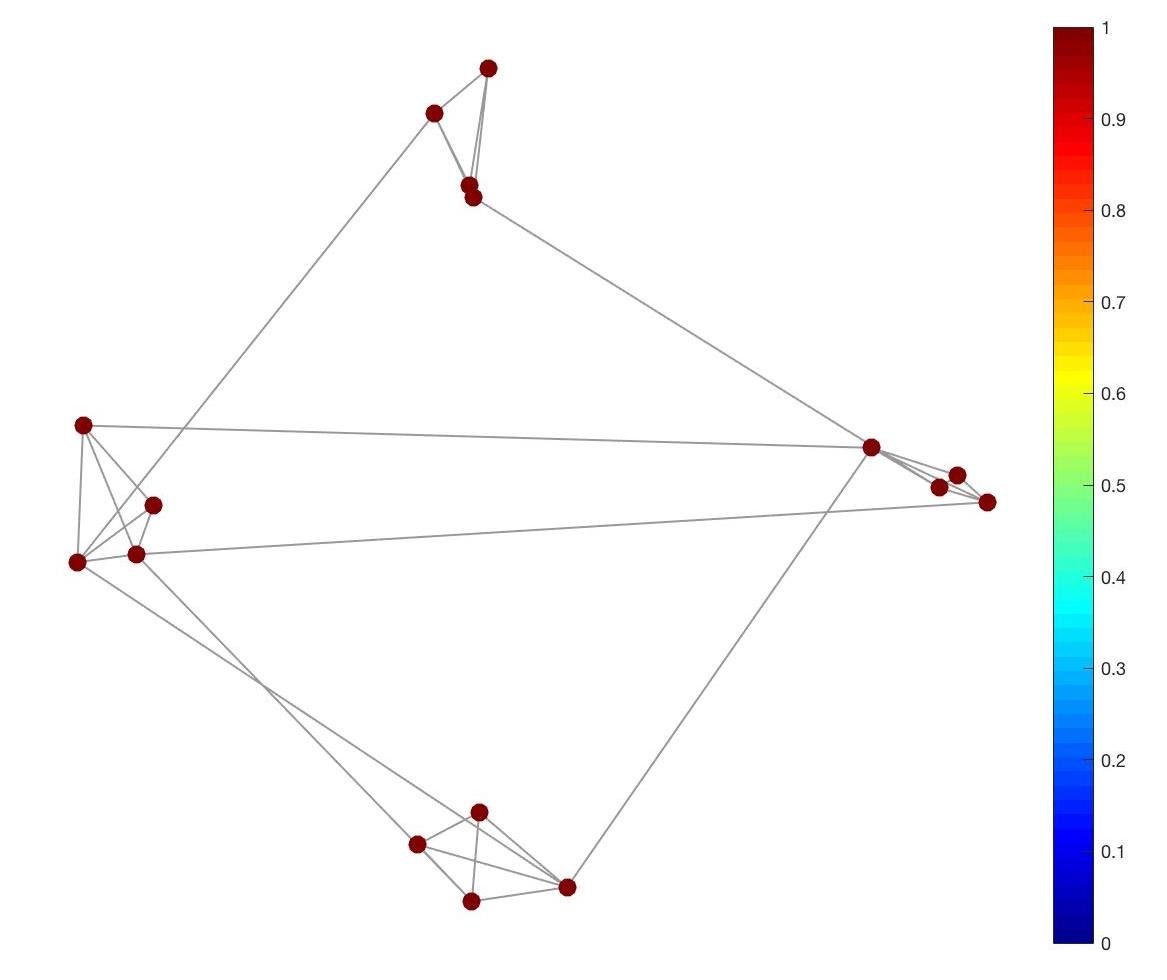
\includegraphics[width=4.5cm,keepaspectratio]{graph} 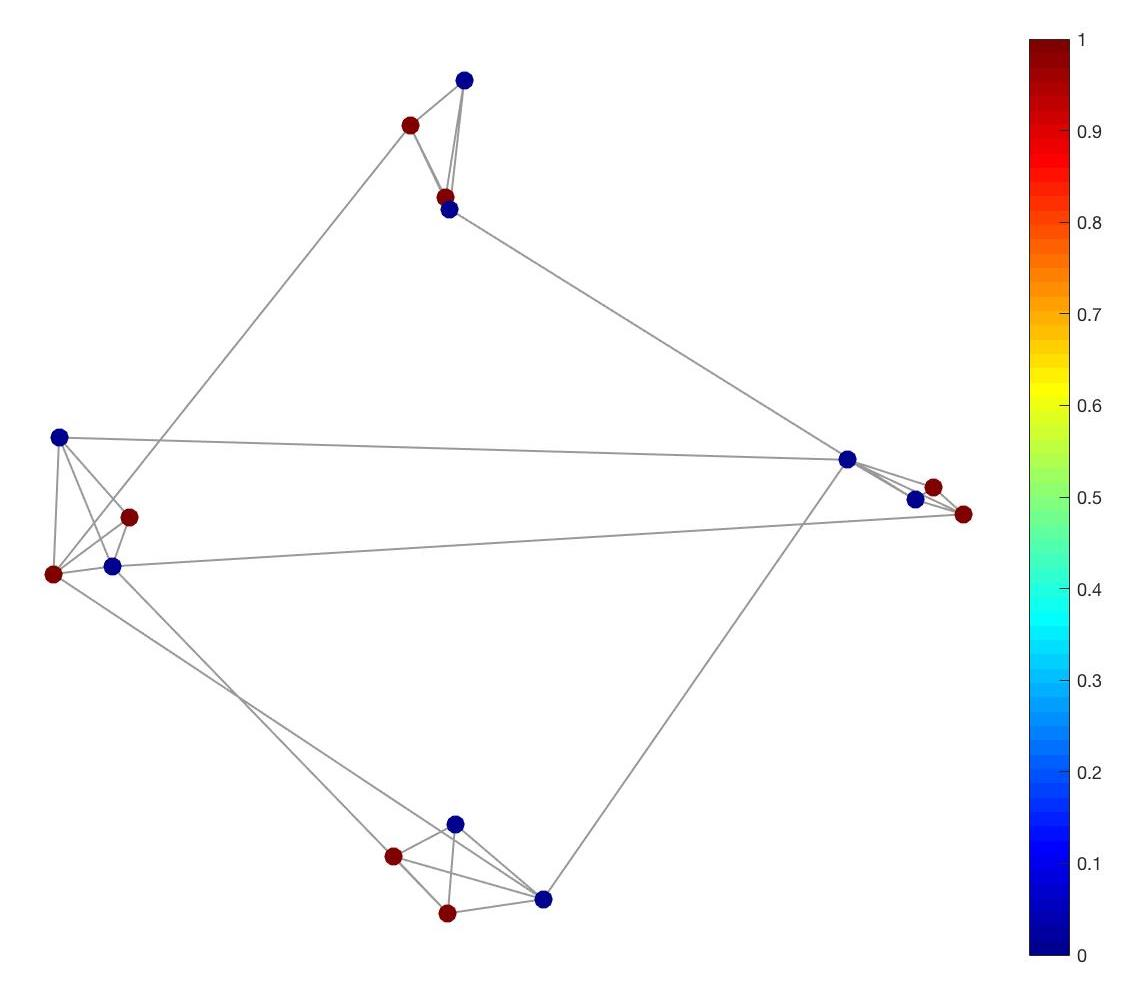
\includegraphics[width=4.5cm,keepaspectratio]{downsample_stage_1} 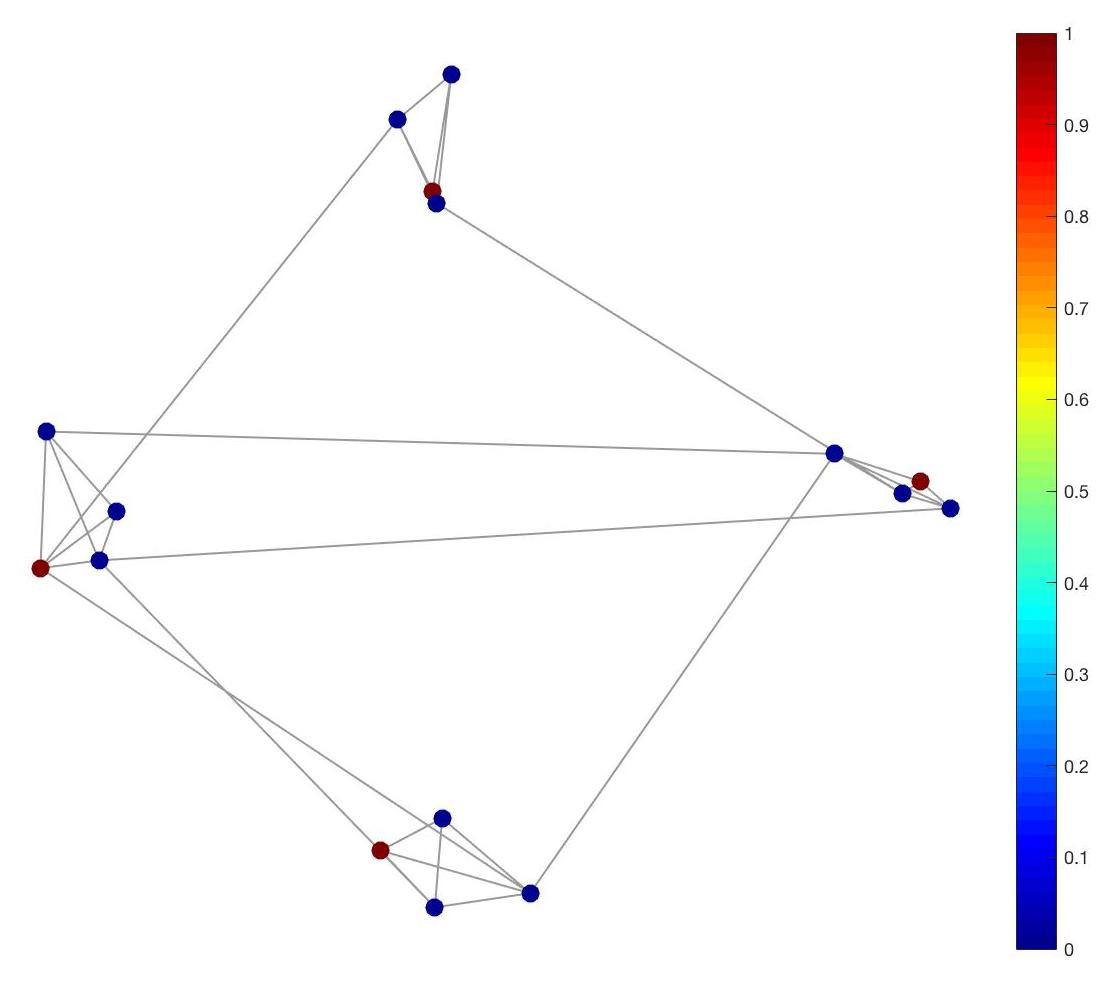
\includegraphics[width=4.5cm,keepaspectratio]{downsample_stage_2}

\caption{\label{fig:Community Graph} Downsampling 16-by-16 community graph. Red vertices are kept after each stage.} {Notice that after 2 stages, 4 kept vertices are from 4 different communities.}
\end{figure}

Dictionary Atoms:

\begin{figure}[H]
\centering

Scaling Function \qquad\qquad\qquad\qquad Wavelet - Scale 1 \qquad\qquad\qquad Wavelet - Scale 2

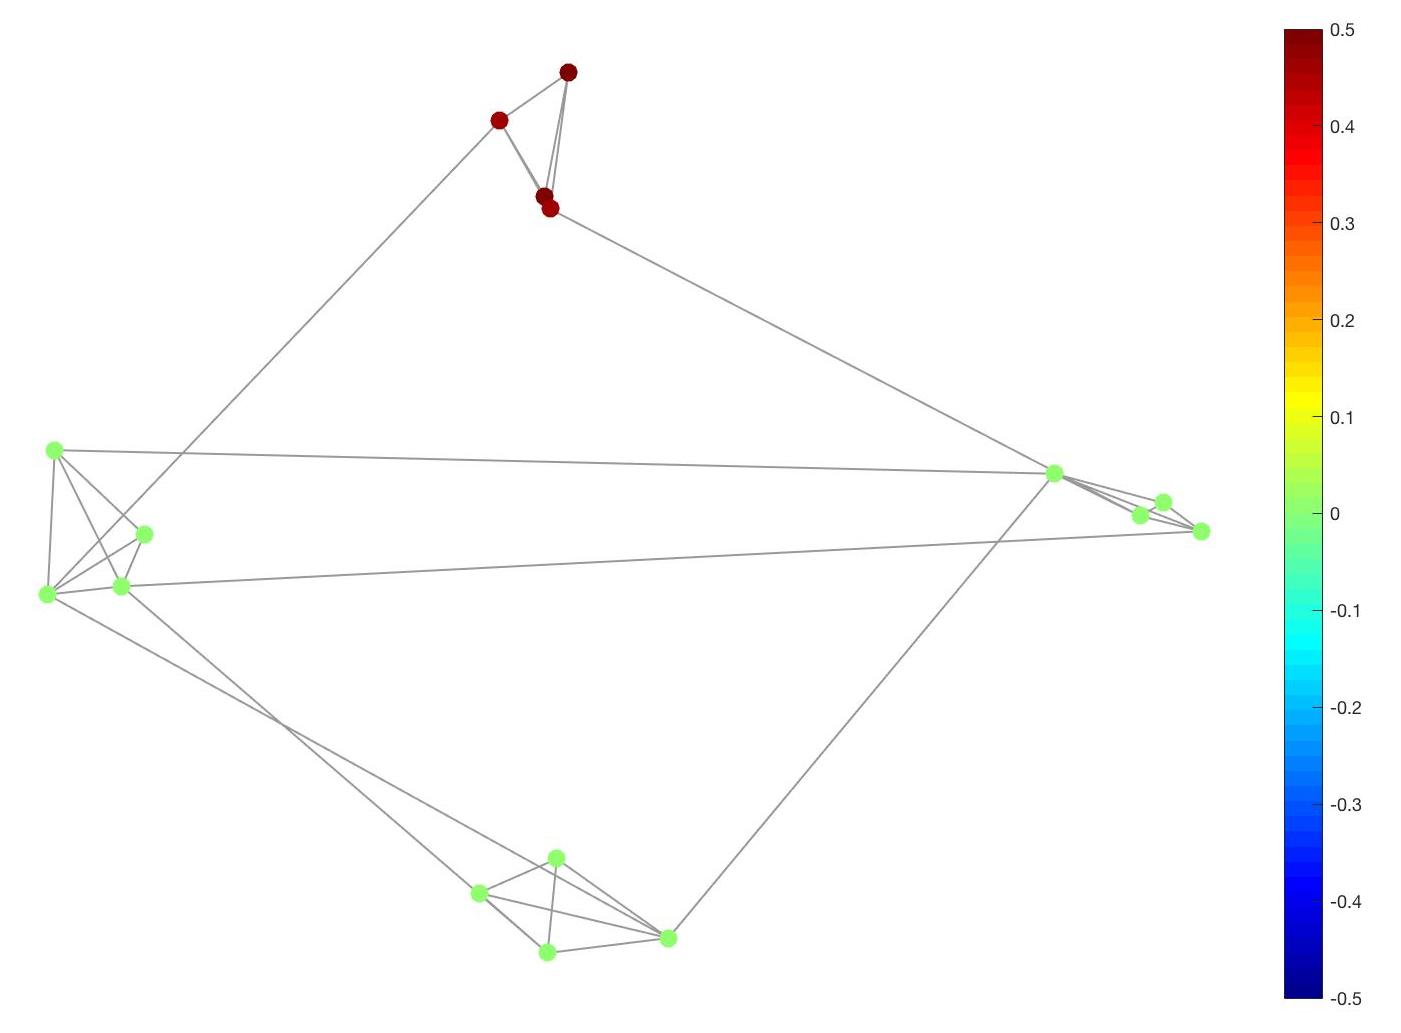
\includegraphics[width=4.75cm,keepaspectratio]{scaling_vertex} 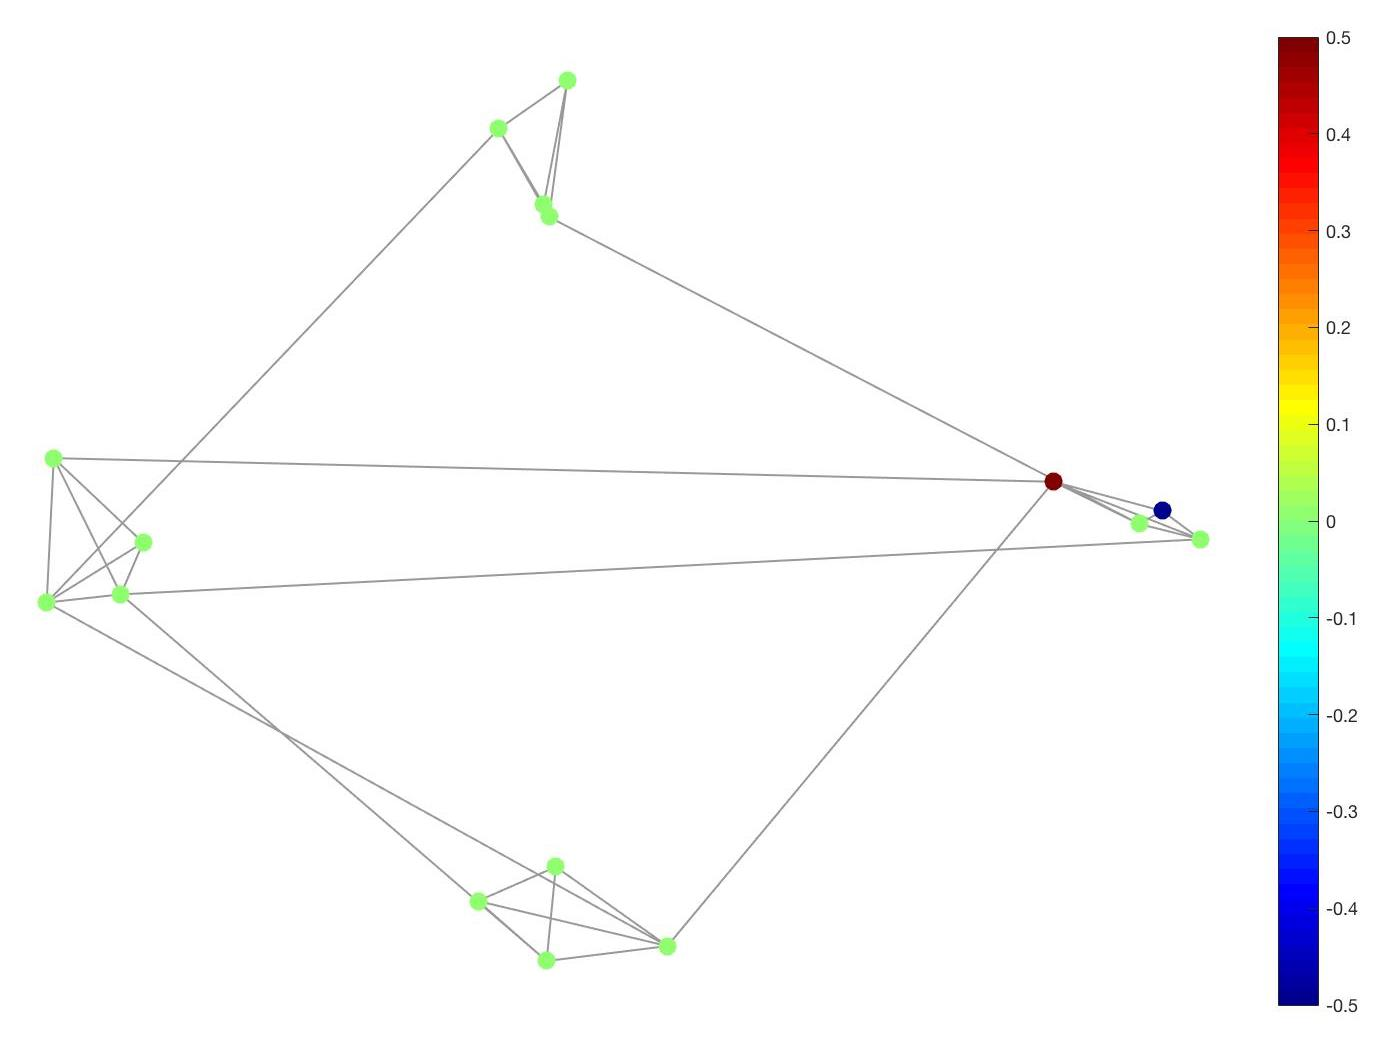
\includegraphics[width=4.75cm,keepaspectratio]{wavelet_scale_1_vertex} 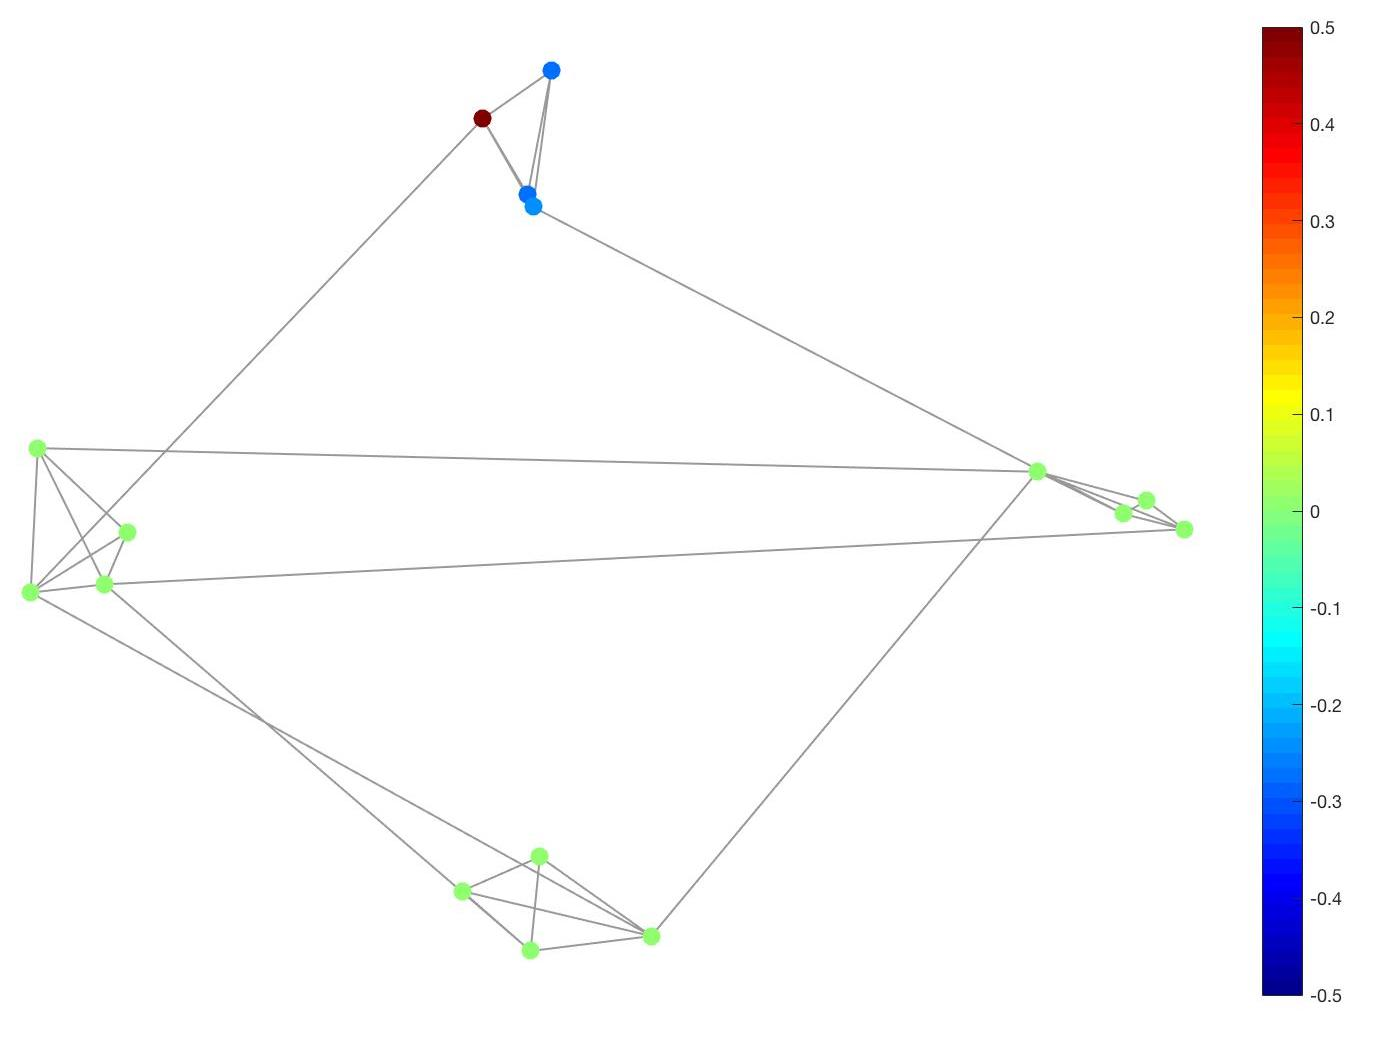
\includegraphics[width=4.75cm,keepaspectratio]{wavelet_scale_2_vertex}

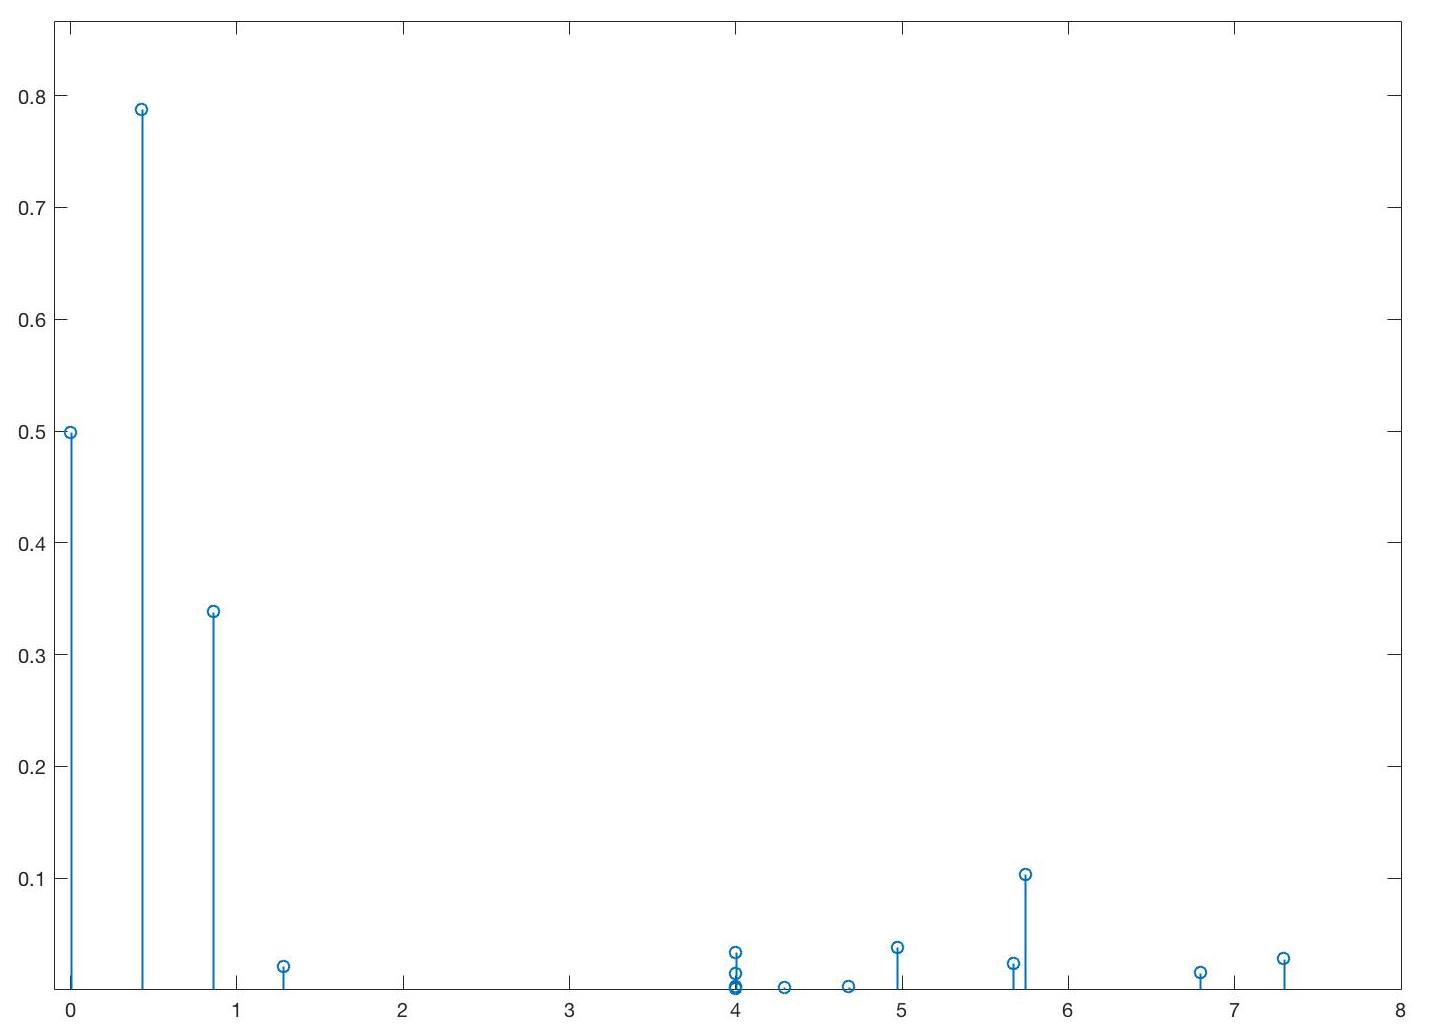
\includegraphics[width=4.75cm,keepaspectratio]{scaling_frequency} 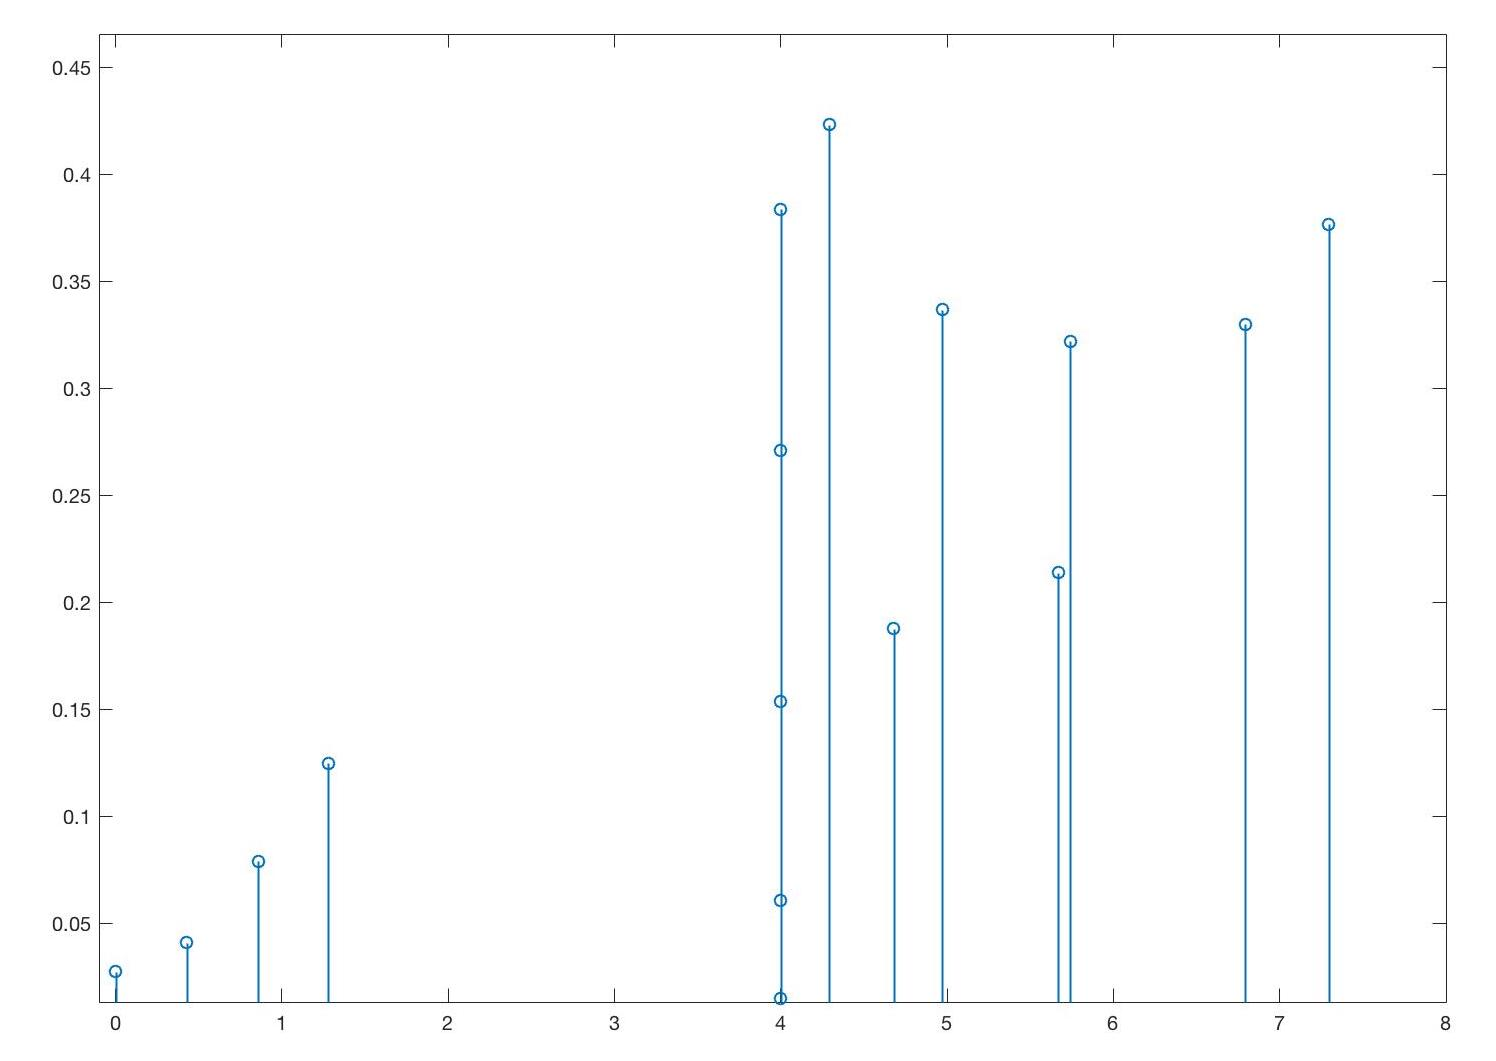
\includegraphics[width=4.75cm,keepaspectratio]{wavelet_scale_1_frequency} 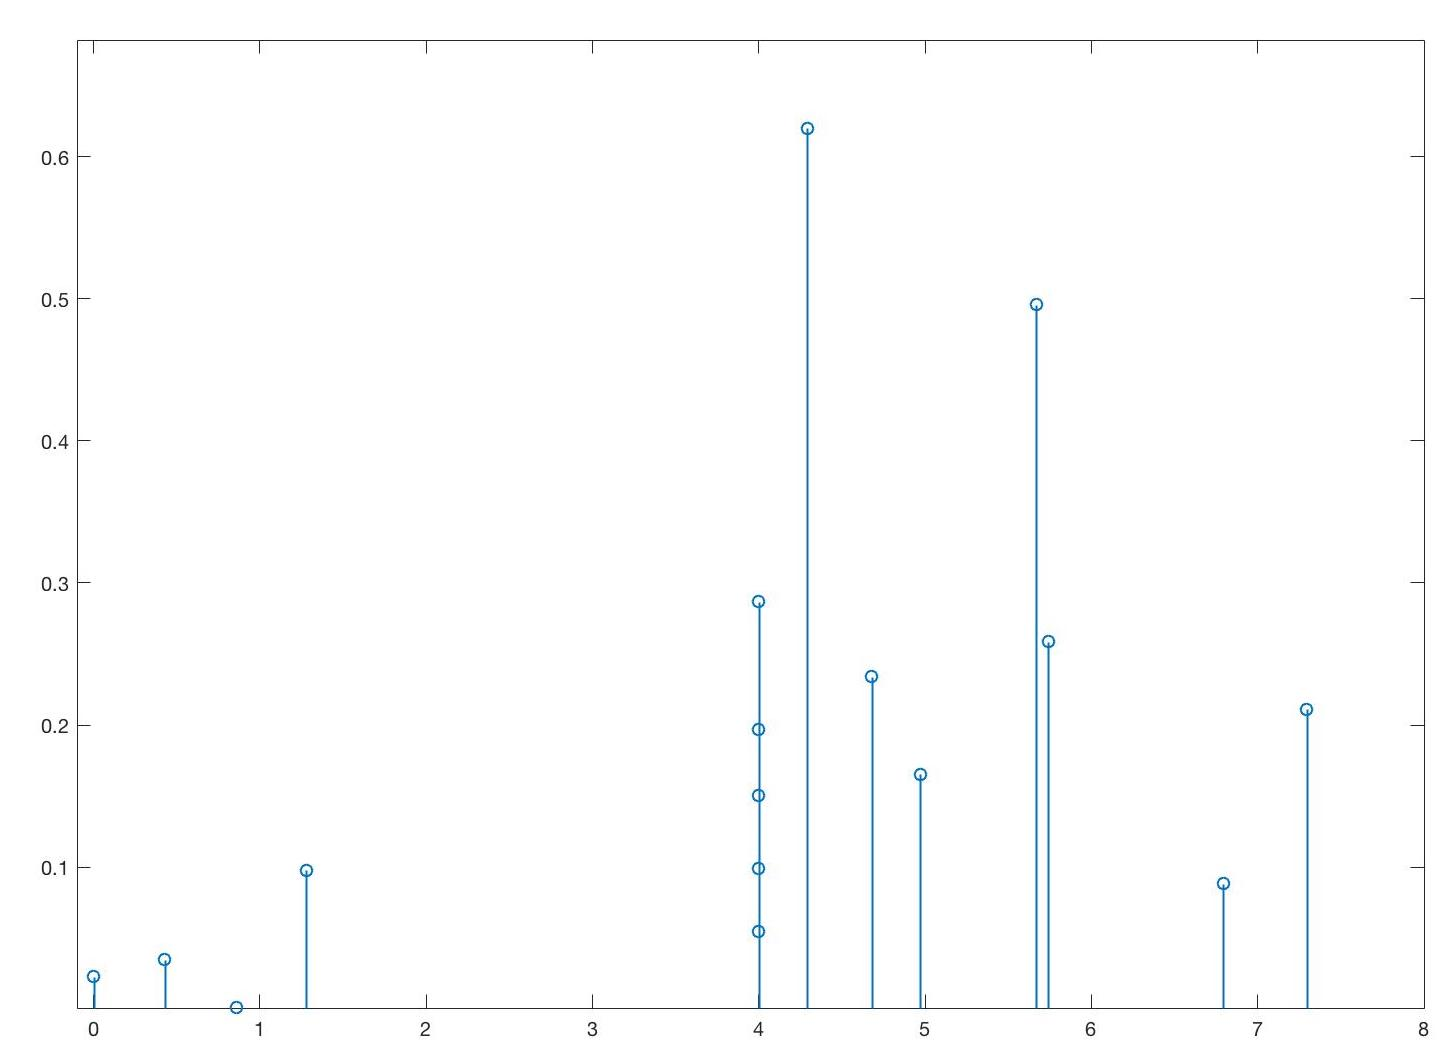
\includegraphics[width=4.75cm,keepaspectratio]{wavelet_scale_2_frequency}

\caption{\label{fig:community dictionary atoms} Dictionary atoms in both vertex and frequency domains.}
\end{figure}


\subsubsection{Example 2: $500\times 500$ Sensor Network}

\begin{figure}[h]
\centering
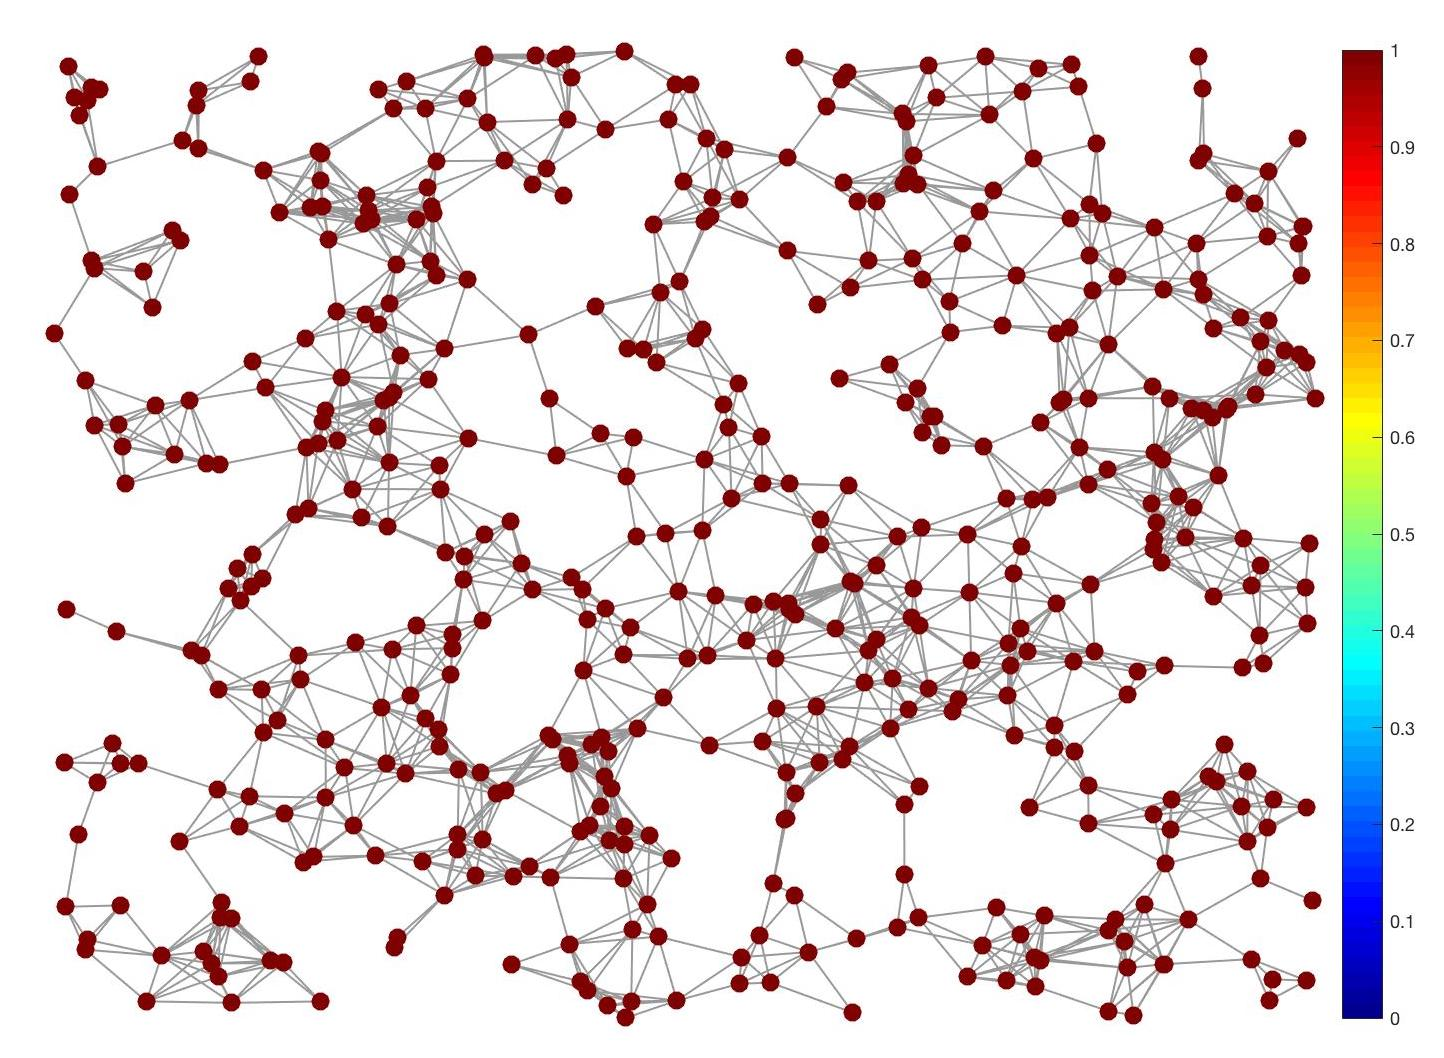
\includegraphics[width=4.84cm,keepaspectratio]{sensor_network/graph} 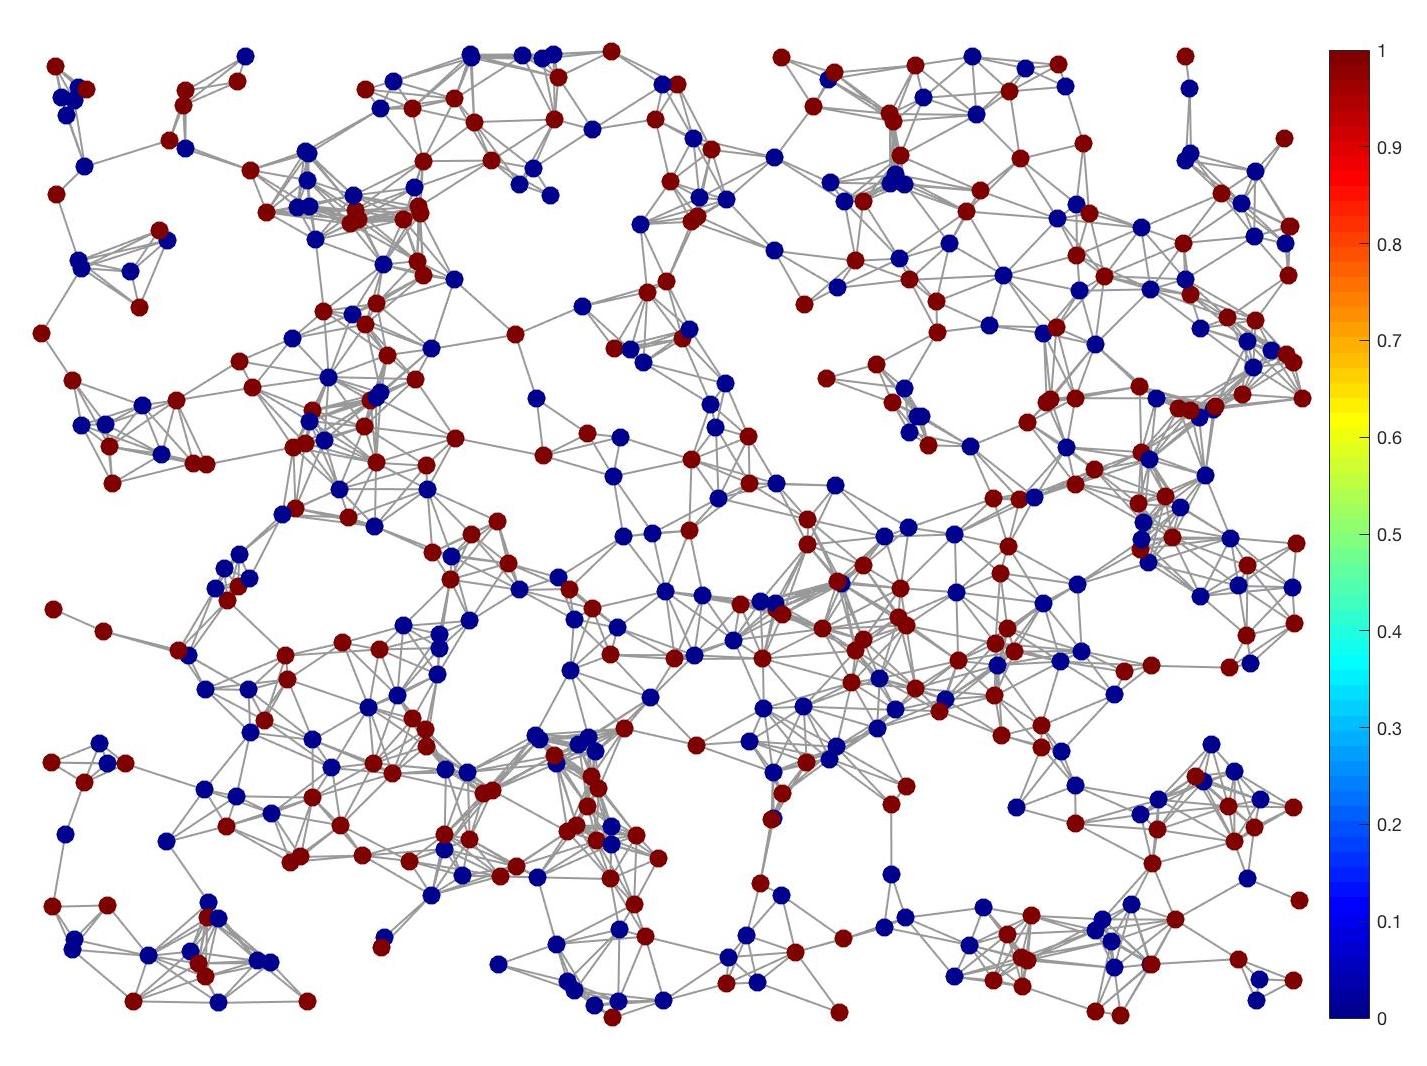
\includegraphics[width=4.85cm,keepaspectratio]{sensor_network/downsample_stage_1} 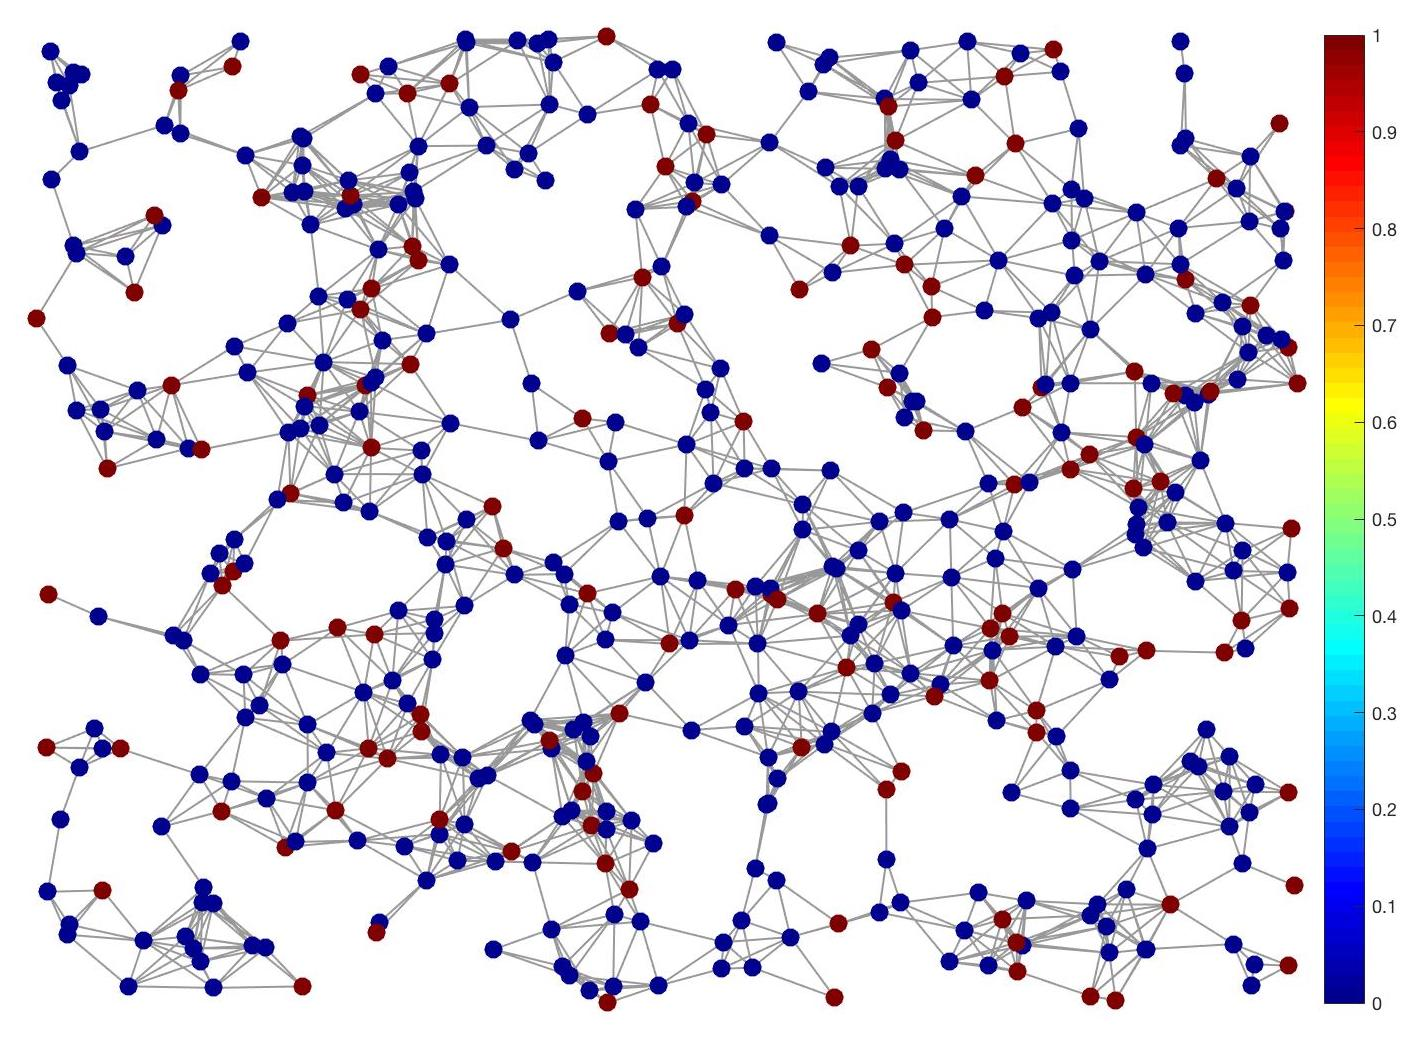
\includegraphics[width=4.85cm,keepaspectratio]{sensor_network/downsample_stage_2}

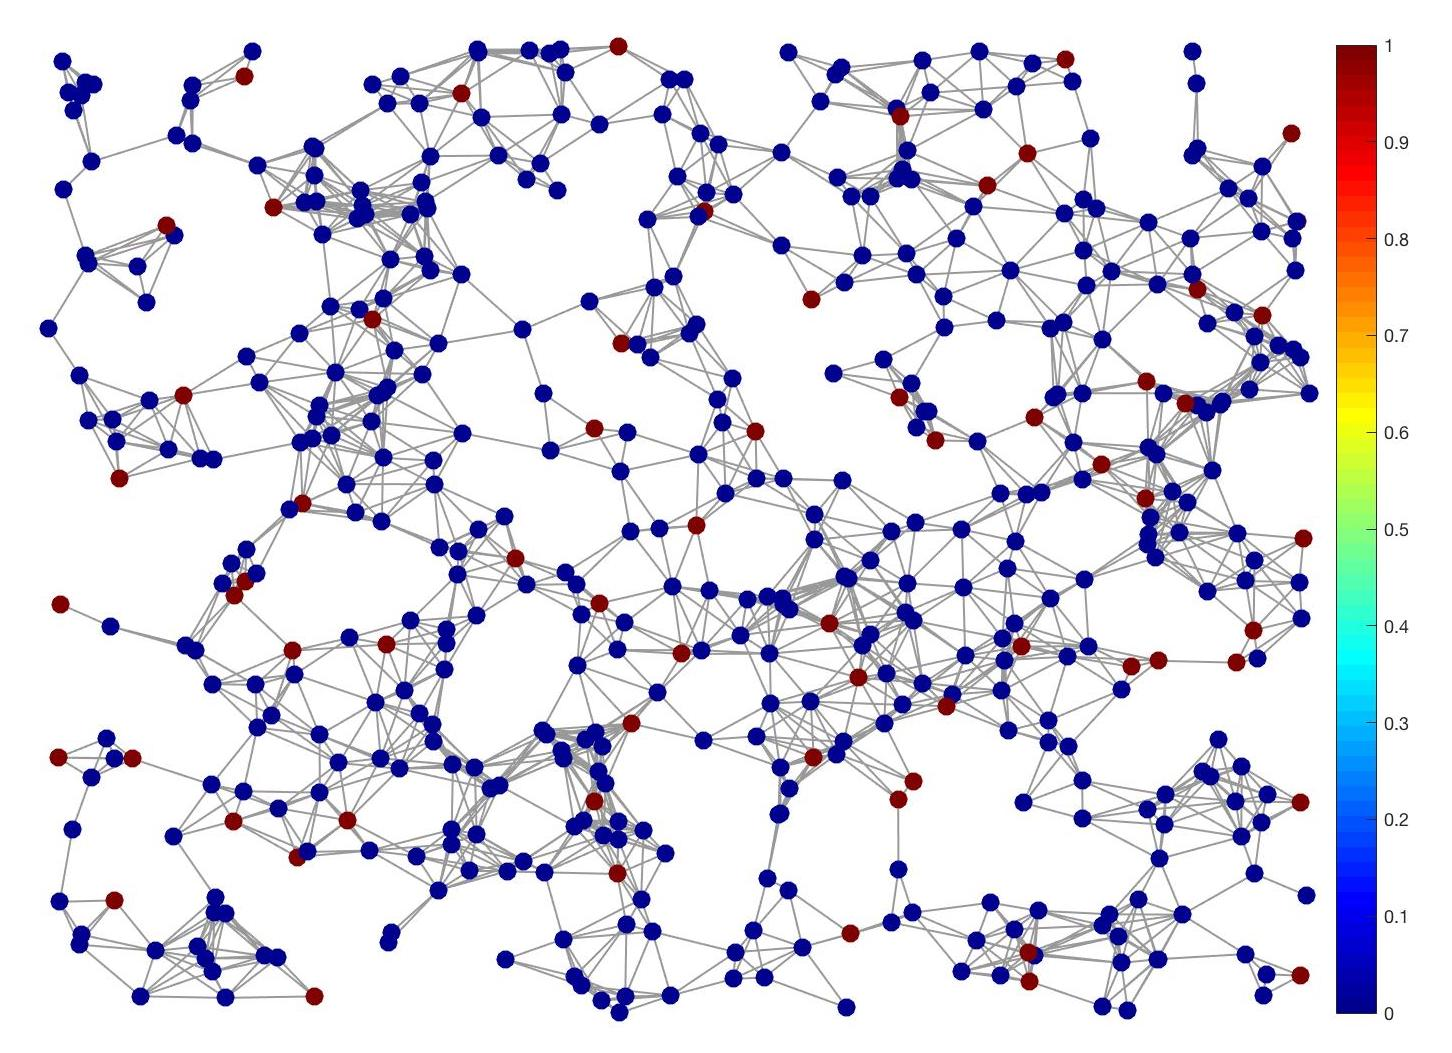
\includegraphics[width=4.84cm,keepaspectratio]{sensor_network/downsample_stage_3} 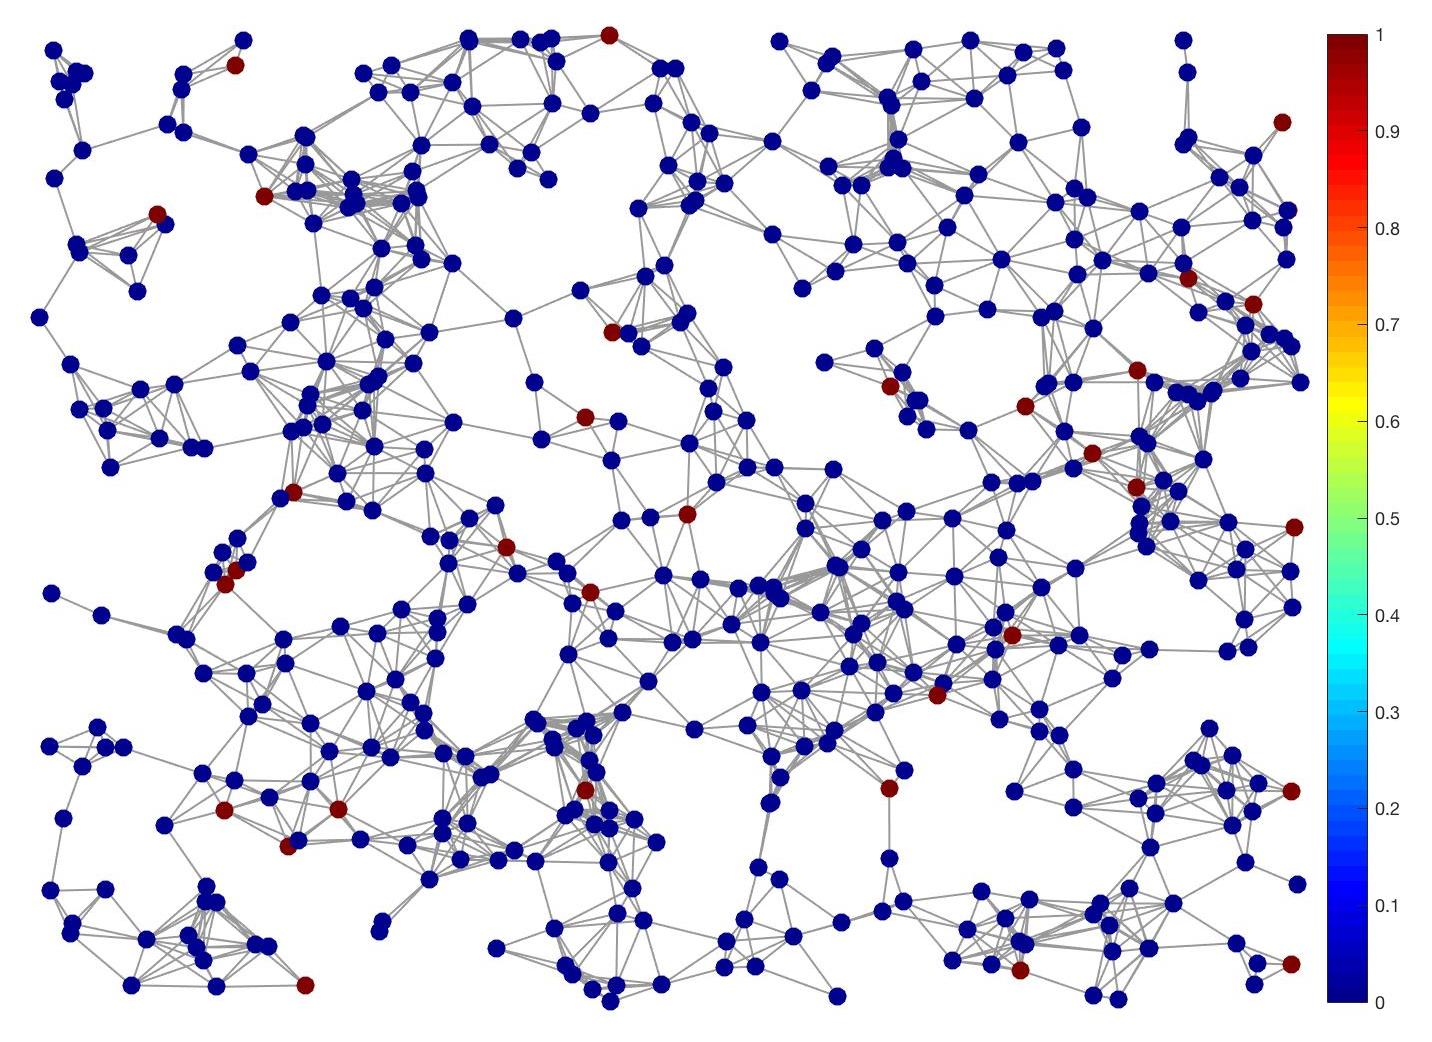
\includegraphics[width=4.85cm,keepaspectratio]{sensor_network/downsample_stage_4} 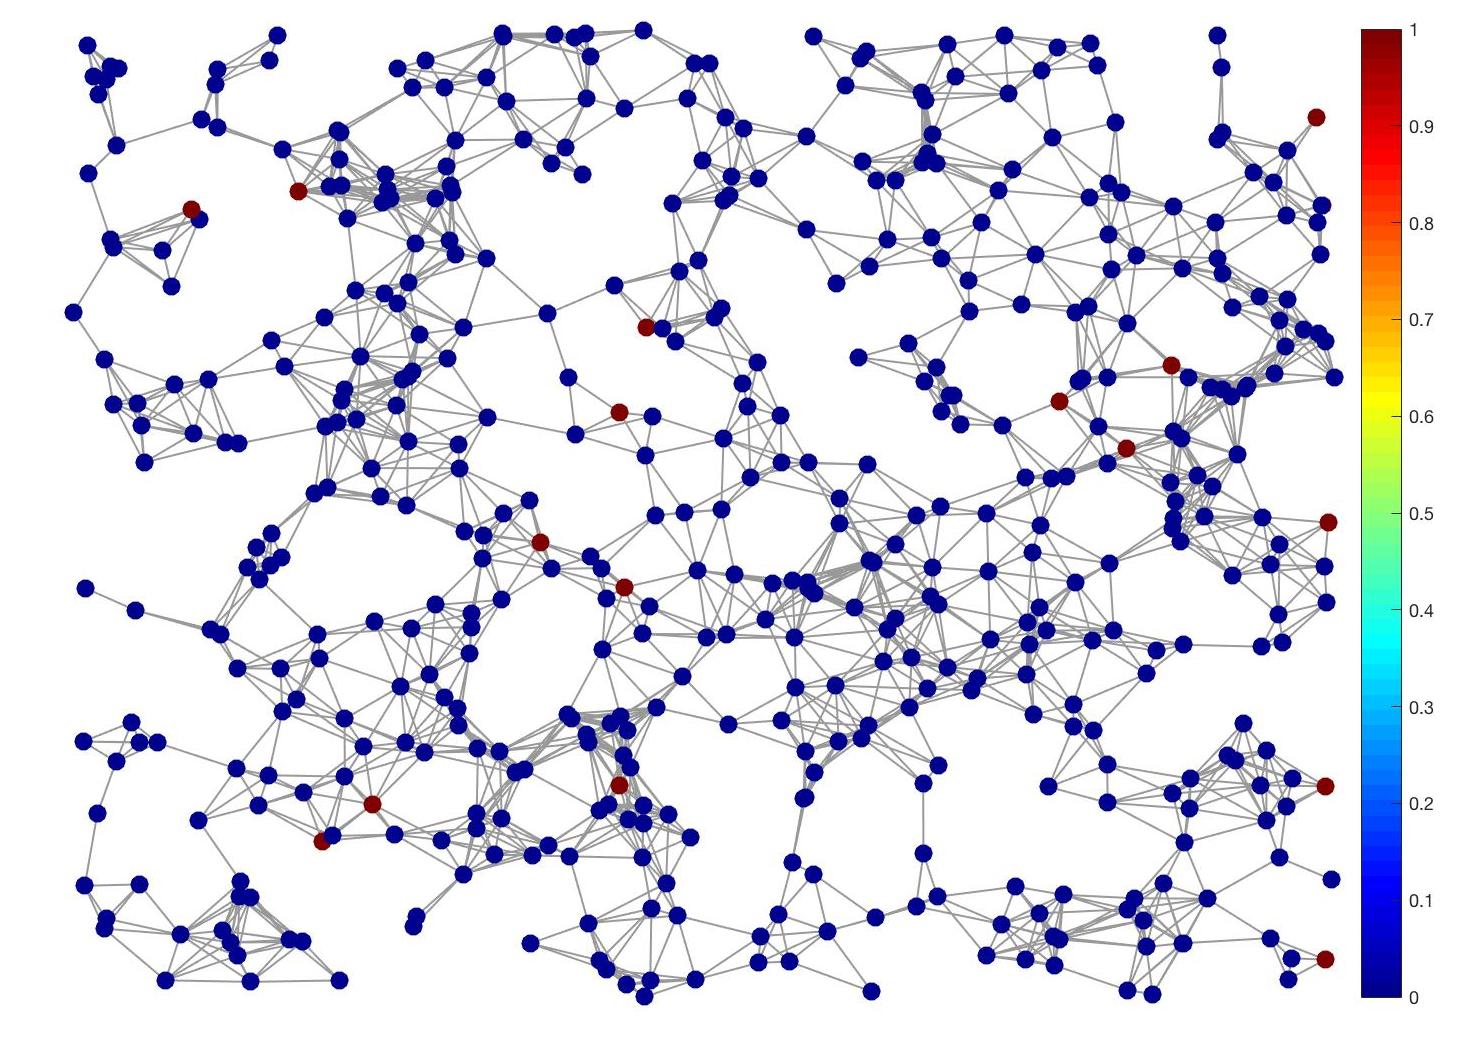
\includegraphics[width=4.85cm,keepaspectratio]{sensor_network/downsample_stage_5}

\caption{\label{fig:sensor network} Downsampling 500-by-500 sensor network.}
{Notice that after each stage, kept vertices cover the whole graph instead of centering at a specific place.}
\end{figure}

Dictionary Atoms:

\begin{figure}[H]
\centering
Scaling Function \qquad\qquad\qquad Wavelet Scale 1 \qquad\qquad\qquad Wavelet Scale 2

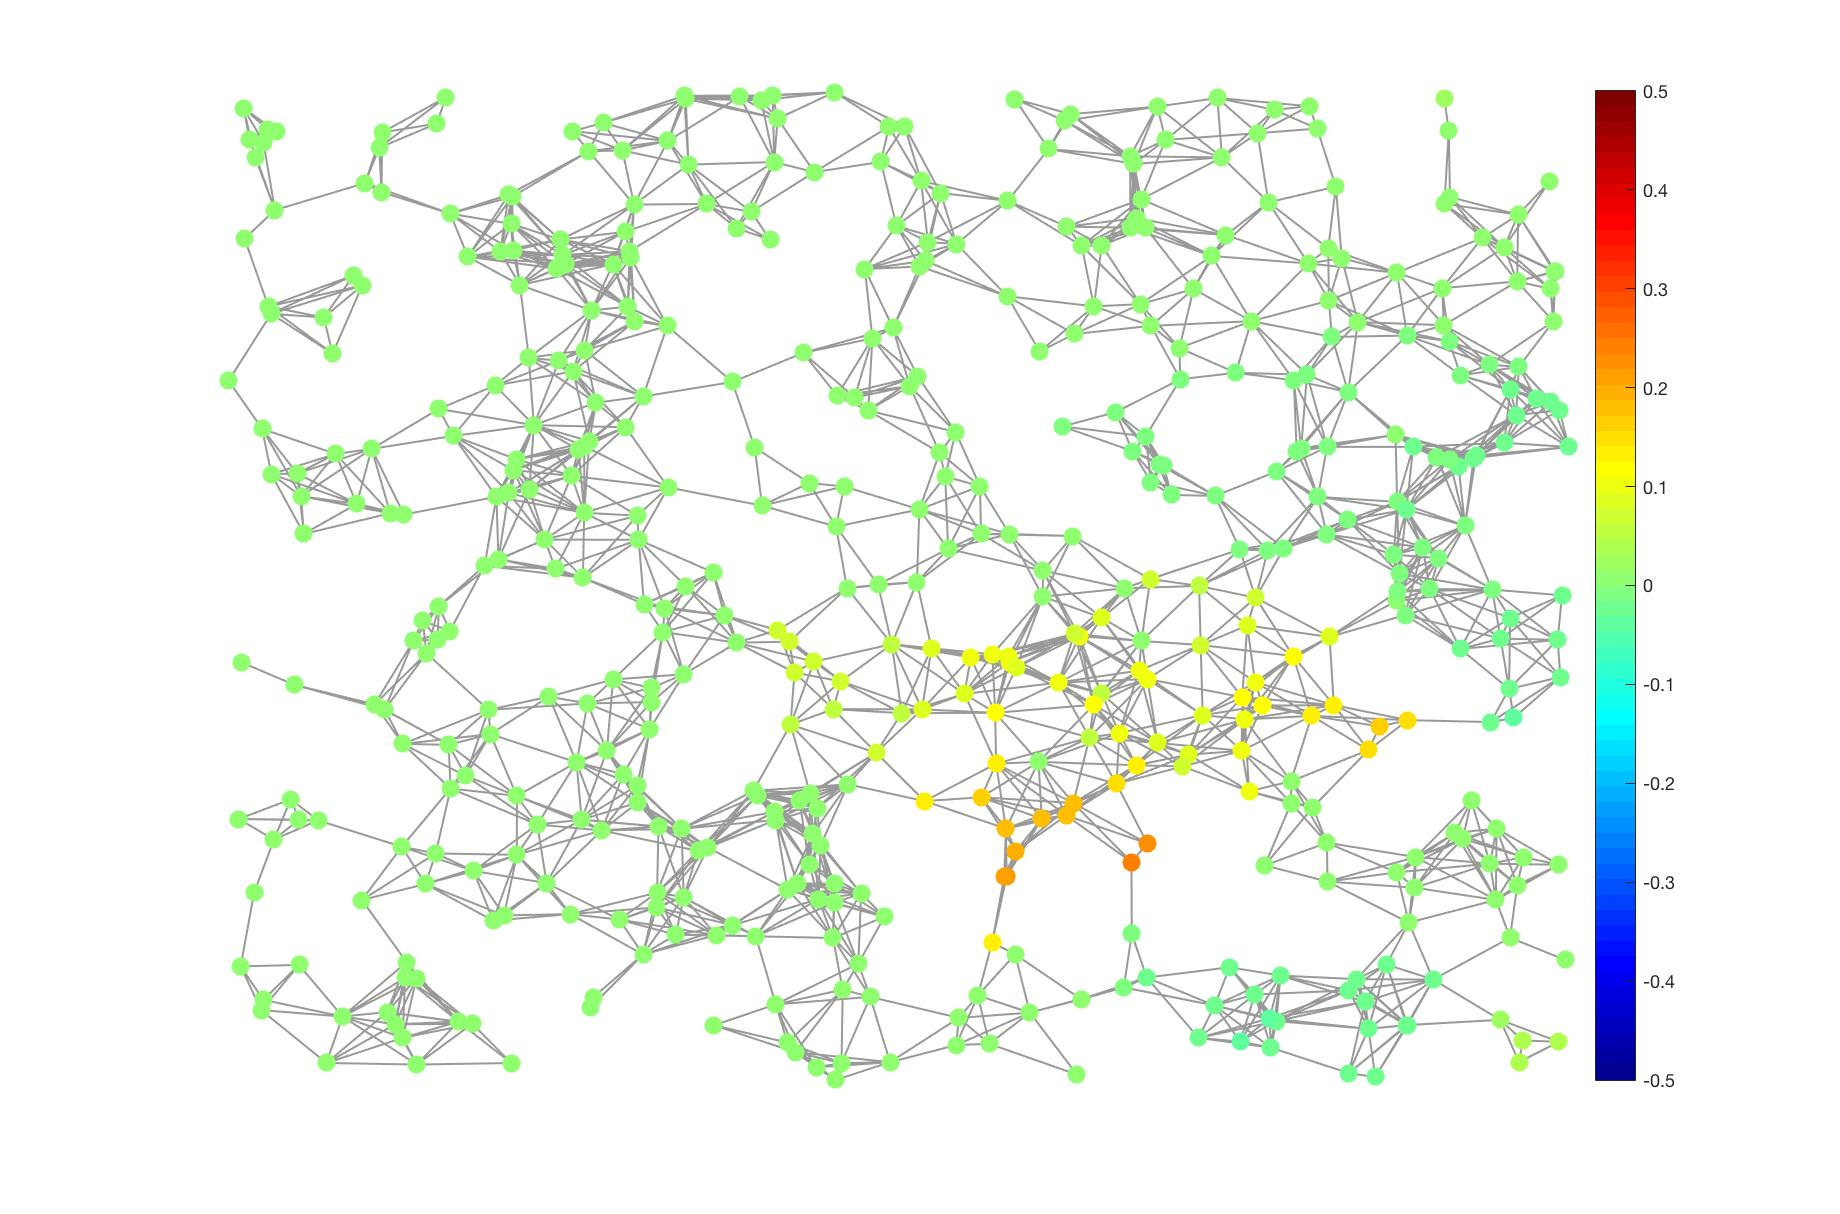
\includegraphics[width=4.84cm,keepaspectratio]{sensor_network/scaling} 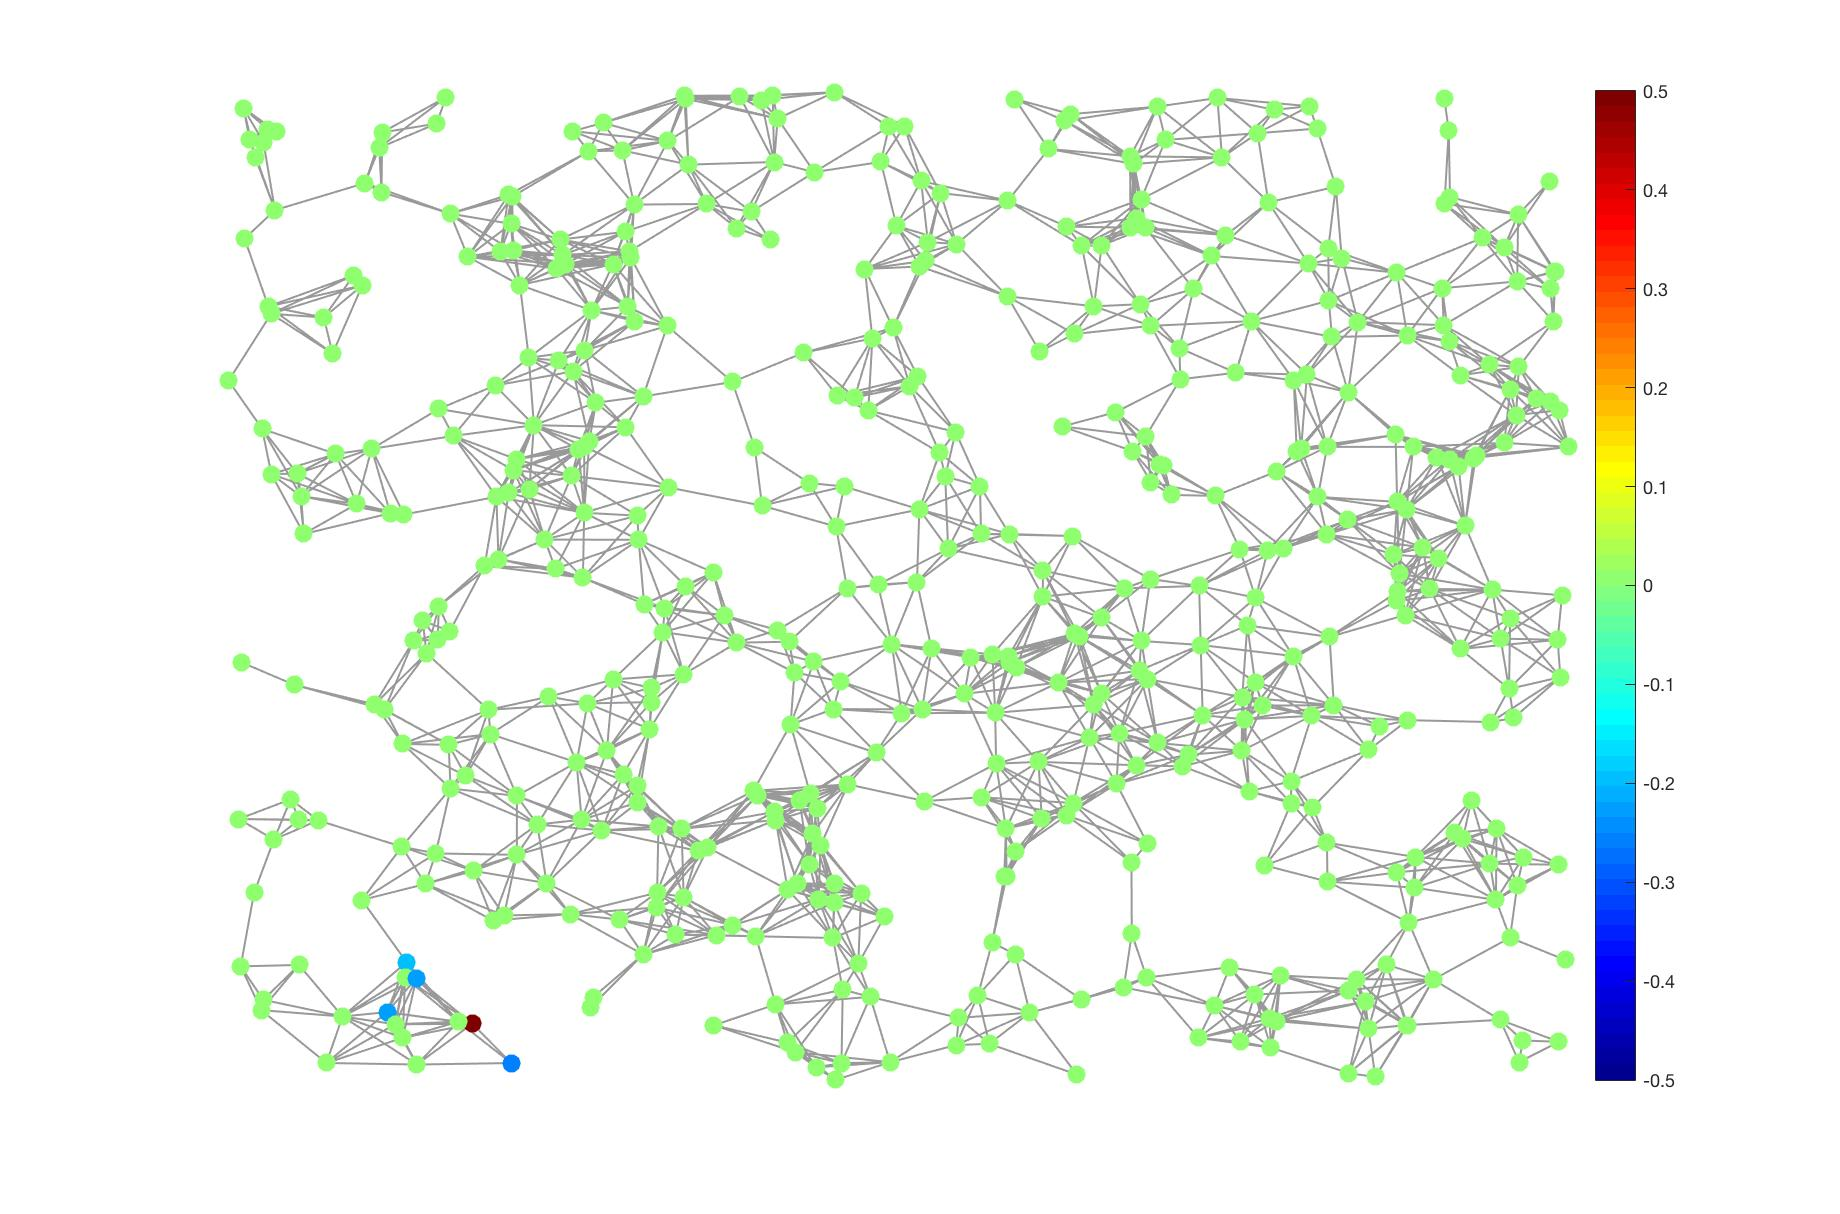
\includegraphics[width=4.85cm,keepaspectratio]{sensor_network/wavelet_scale_1_vertex} 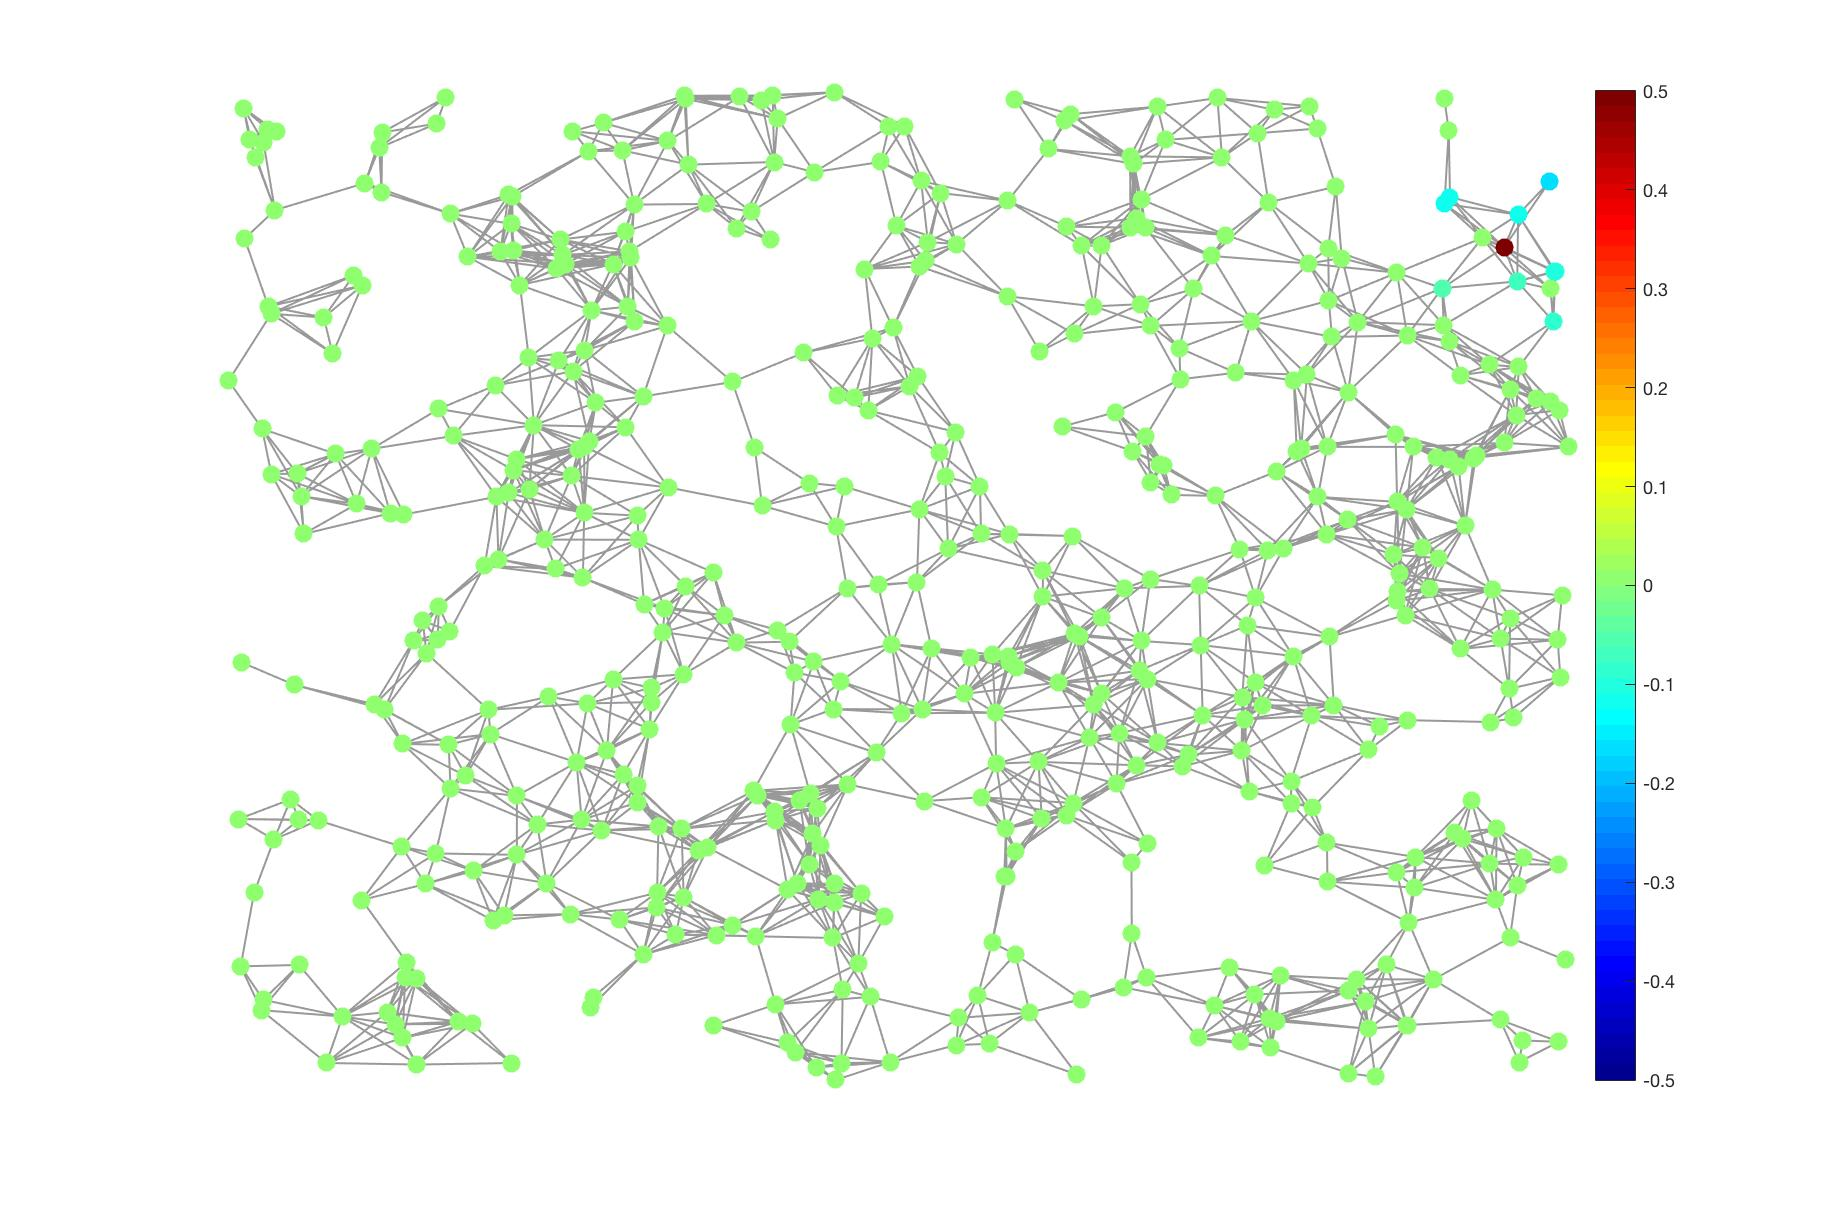
\includegraphics[width=4.85cm,keepaspectratio]{sensor_network/wavelet_scale_2_vertex}

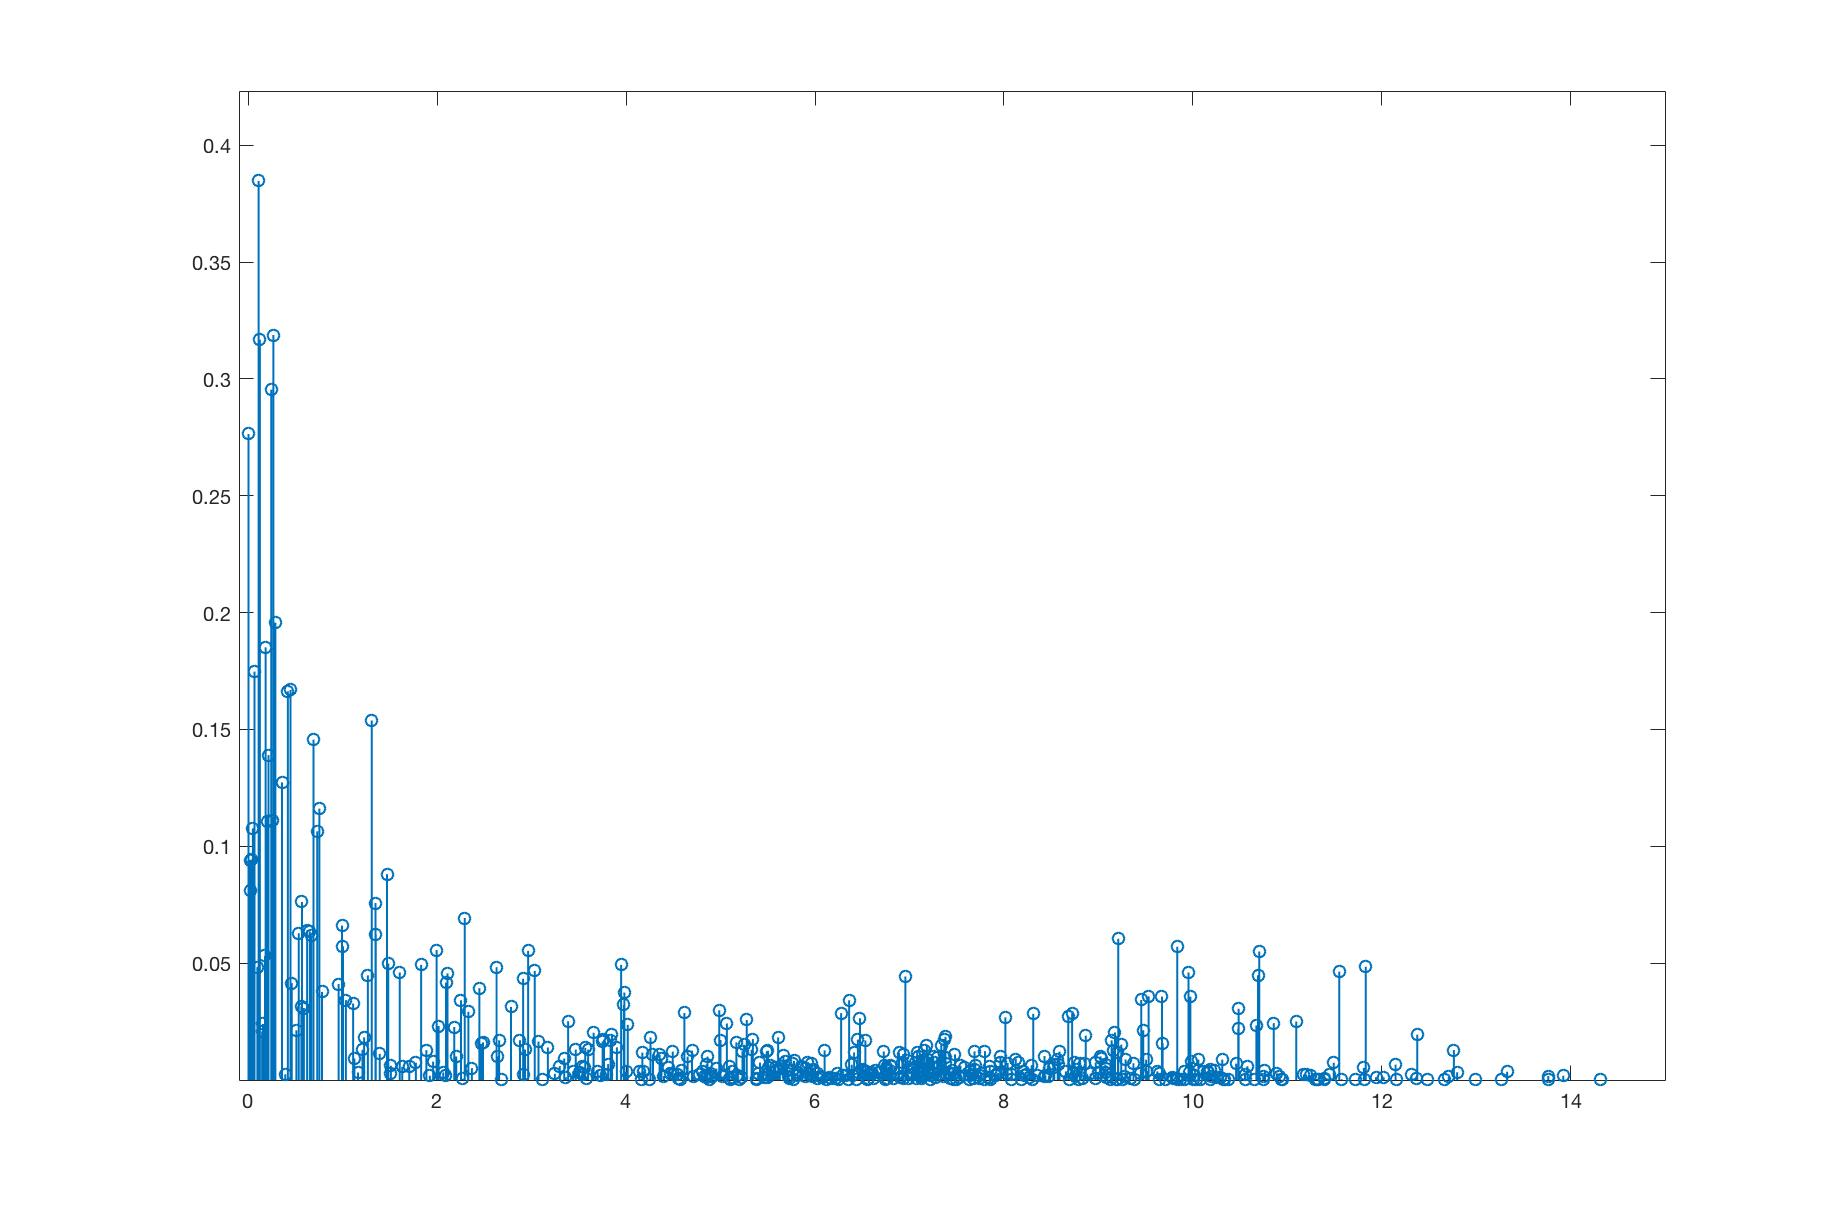
\includegraphics[width=4.84cm,keepaspectratio]{sensor_network/scaling_frequency} 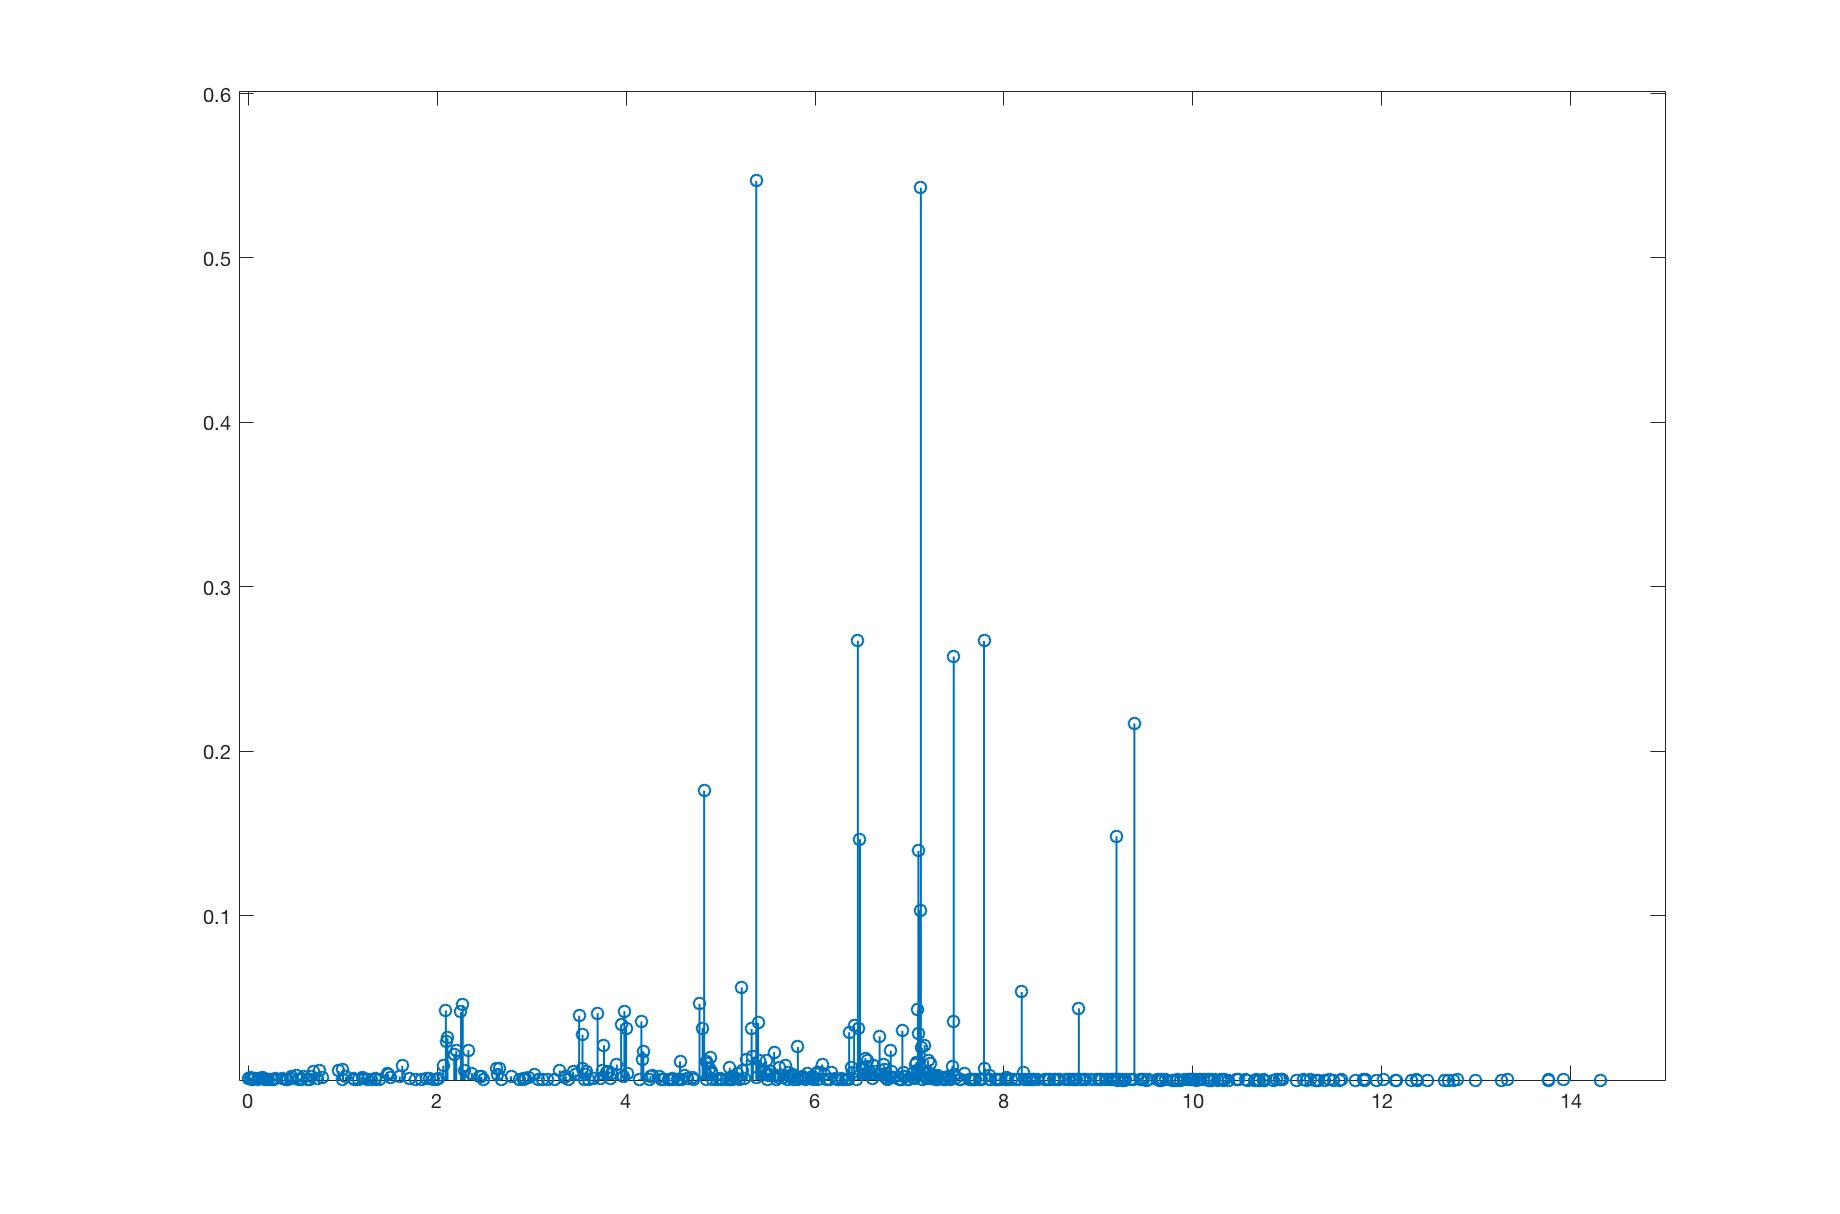
\includegraphics[width=4.85cm,keepaspectratio]{sensor_network/wavelet_scale_1_frequency} 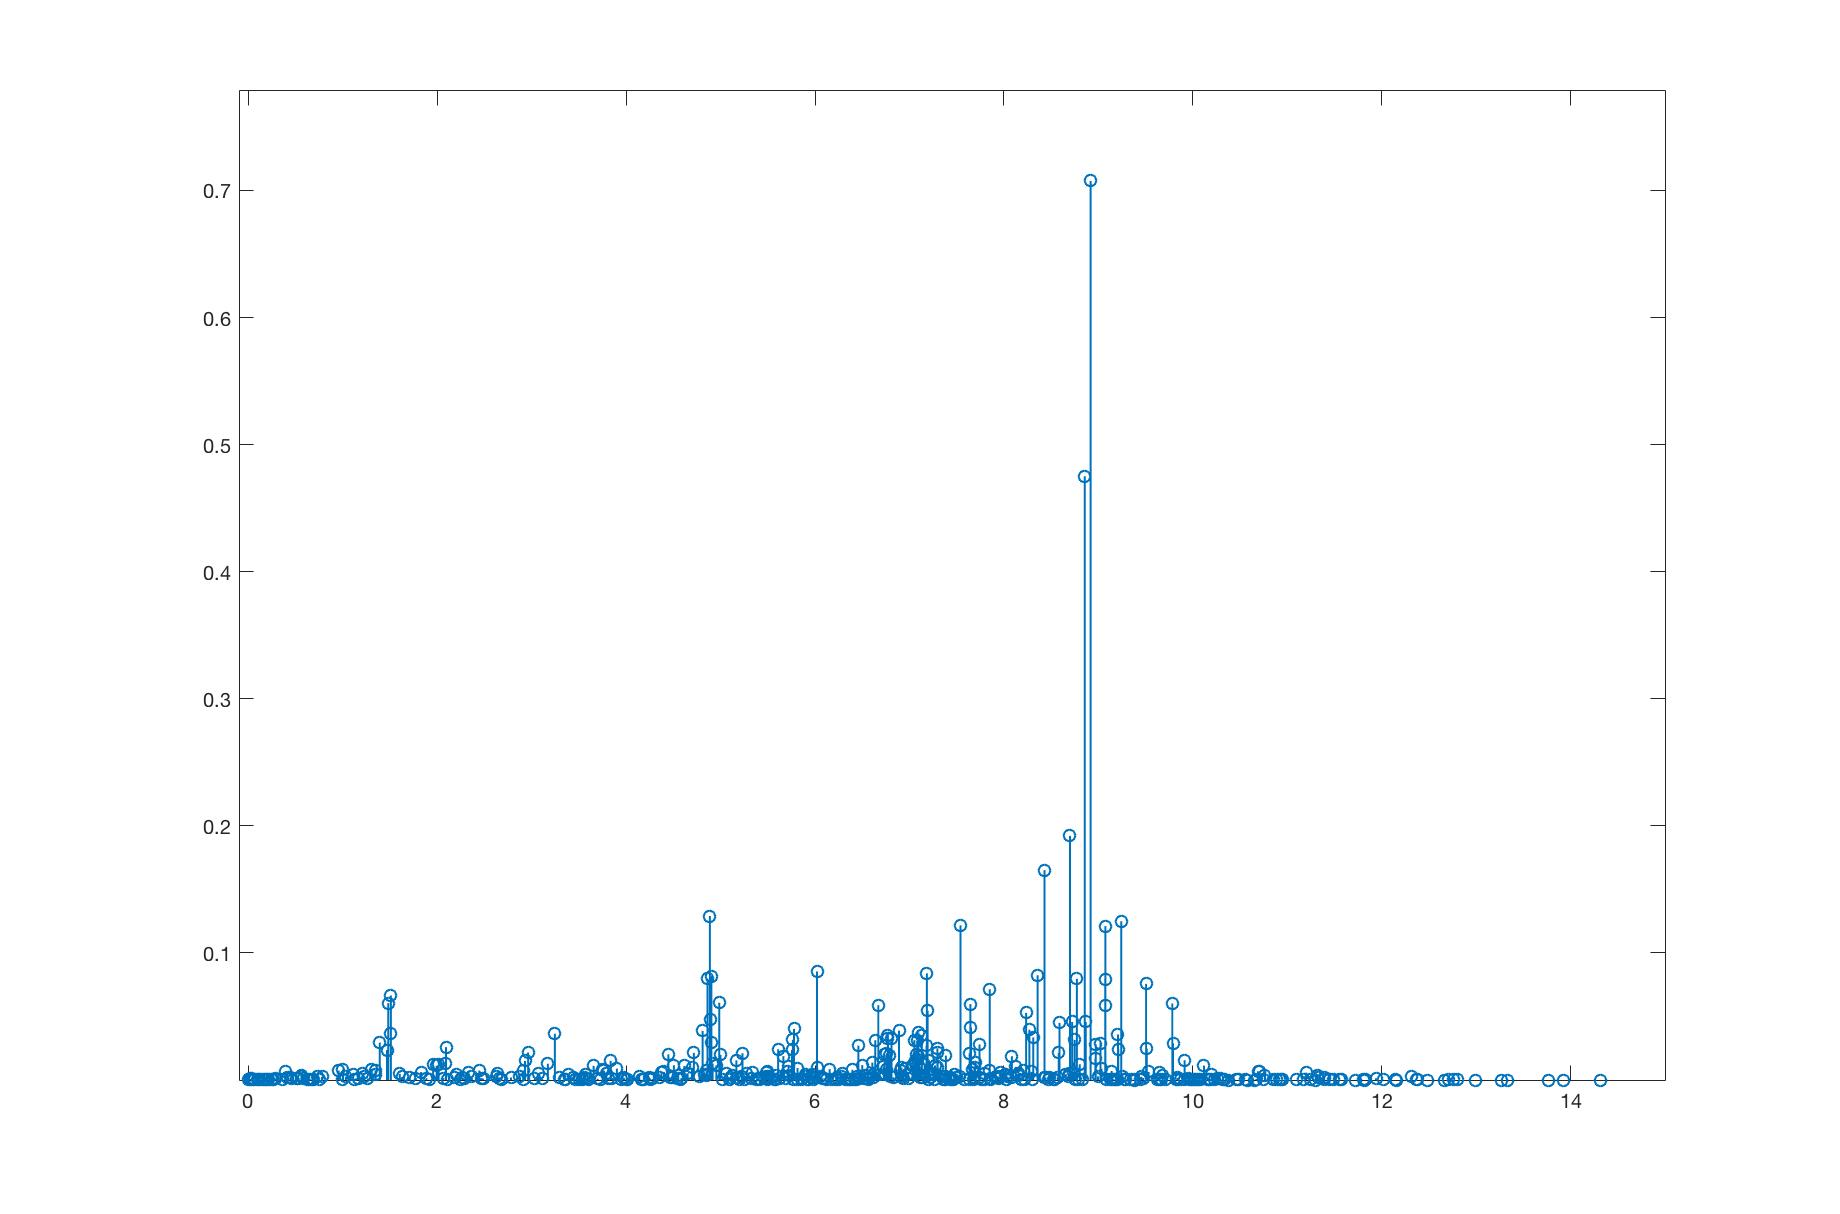
\includegraphics[width=4.85cm,keepaspectratio]{sensor_network/wavelet_scale_2_frequency}

\caption{\label{fig:sensor net} Dictionary Atoms in both vertex and frequency domain.}
\end{figure}



\section{pMMF-Graph Reduction}

\subsection{MMF on diffusion operator - June 8-12}
Given graph $G$, let $G.U$ be eigenvectors of its graph Laplacian and $G.e$ be corresponding eigenvectors. Let $A = G.U*f(G.e)*G.U^T$, where $f(\lambda) = e^{-\tau\lambda}$. One level of MMF on matrix $A$ results in

$$H = P_2Q_1AQ_1^TP_2^T$$

Assume $H$ is a diffusion operator on some reduced graph. 

Tried to (not sure if it's even a valid method):

\begin{enumerate}
\item Diagonalize $H = VDV^T$
\item Construct a graph Laplacian $L = Vf^{-1}(D)V^T$
\end{enumerate}

Failed: $L$ is not a Laplacian on downsampled vertices.

\smallskip
Random thoughts:
\begin{enumerate}
\item Are there any methods to construct a graph Laplacian from $H$? 
\item Find $L$ s.t. minimizes $|f(L) - H|$ ?
\end{enumerate}


\subsection{MMF on weighted adjacency matrix $W$ - June 12}
Some general observations:
\begin{enumerate}
\item The core $H$ has non-zero diagonals.
\item The new graph is not necessarily connected.
\item The new graph is still pretty sparse.

\item The current clustering method doesn't yield great downsampling results for path and ring graphs. 

\item The clusters have great influences on how downsampled graphs are rewired.
\end{enumerate}

\subsubsection{Experiments on path graphs}
MMF works well for path graphs in general. The core has zero diagonals and the new graph is connected (if \#clusters = 1). The lowest eigenvector of the reduced Laplacian and of the original Laplacian are both constants.

\begin{figure}[H]
\centering

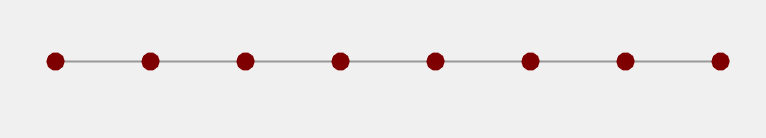
\includegraphics[width = 8cm]{path_graph/path_graph}

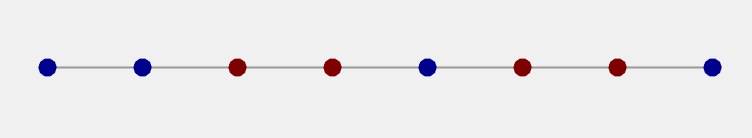
\includegraphics[width = 8cm]{path_graph/downsample_path_graph}

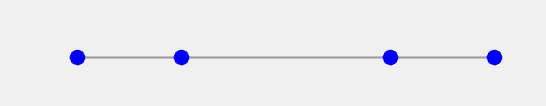
\includegraphics[width = 8cm]{path_graph/rewire_path_graph}

\caption{a.original graph b.downsampled graph(red vertices are kept) c. reduced graph}
\end{figure}


\subsubsection{Experiments on ring graphs}
For ring graphs, the core has zero diagonals, but the new graph is not necessarily connected. The new graph captures the ring structure. The lowest eigenvector of the reduced Laplacian and of the original Laplacian are both constants.
\begin{figure}[H]
\centering

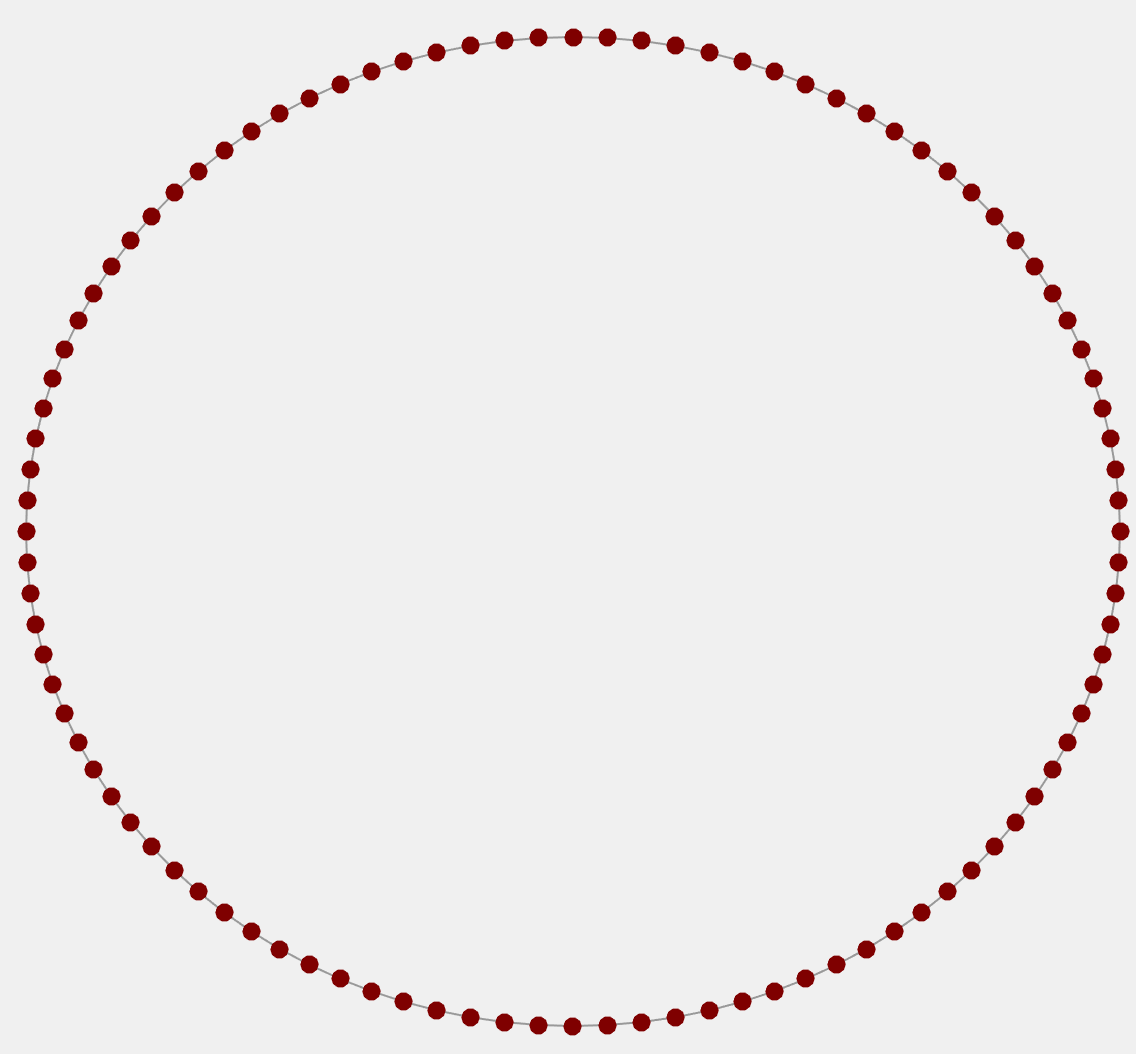
\includegraphics[width = 6cm]{ring_graph/ring_graph}
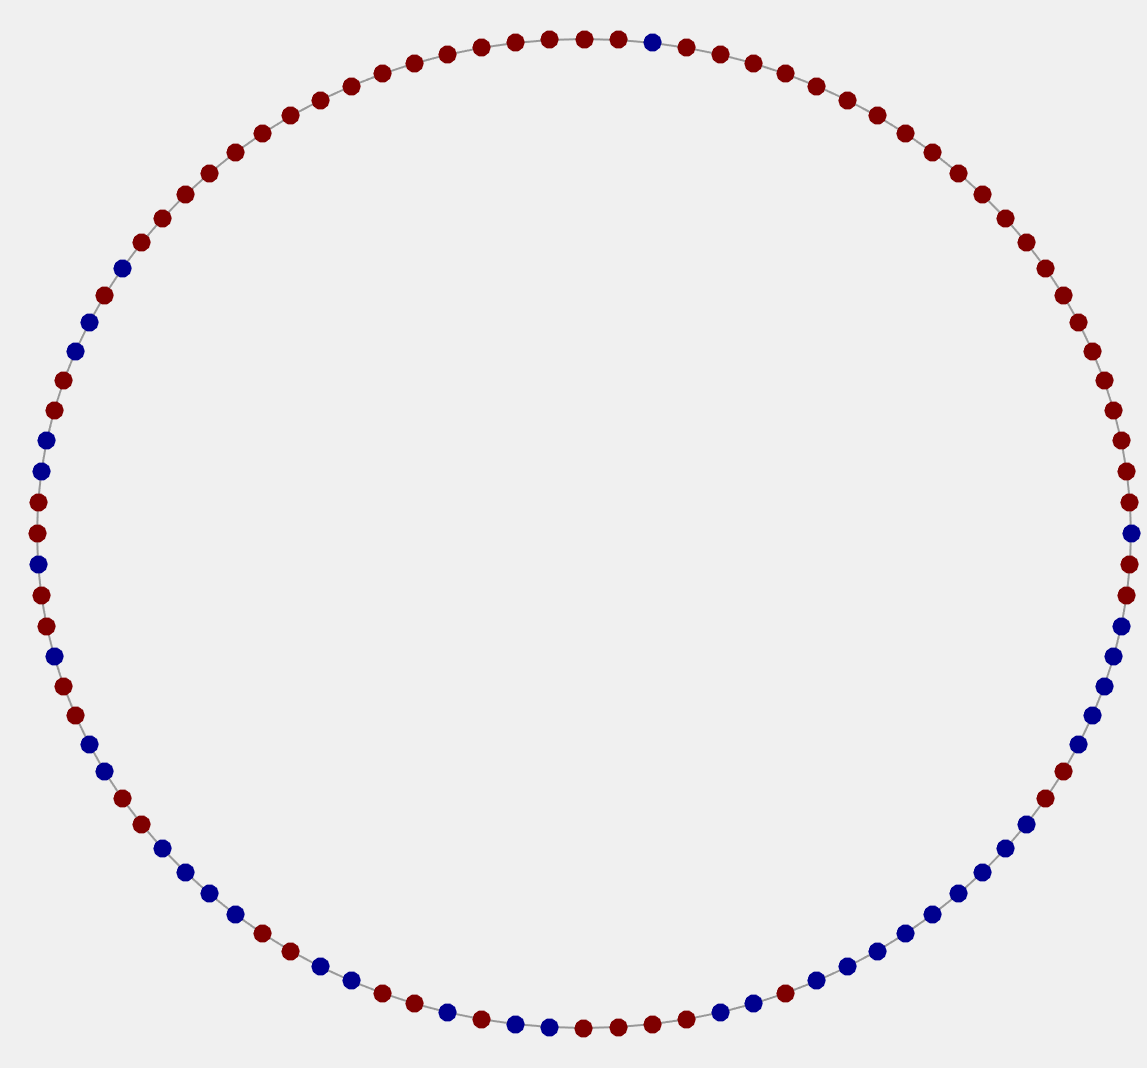
\includegraphics[width = 6cm]{ring_graph/ring_graph_downsample}
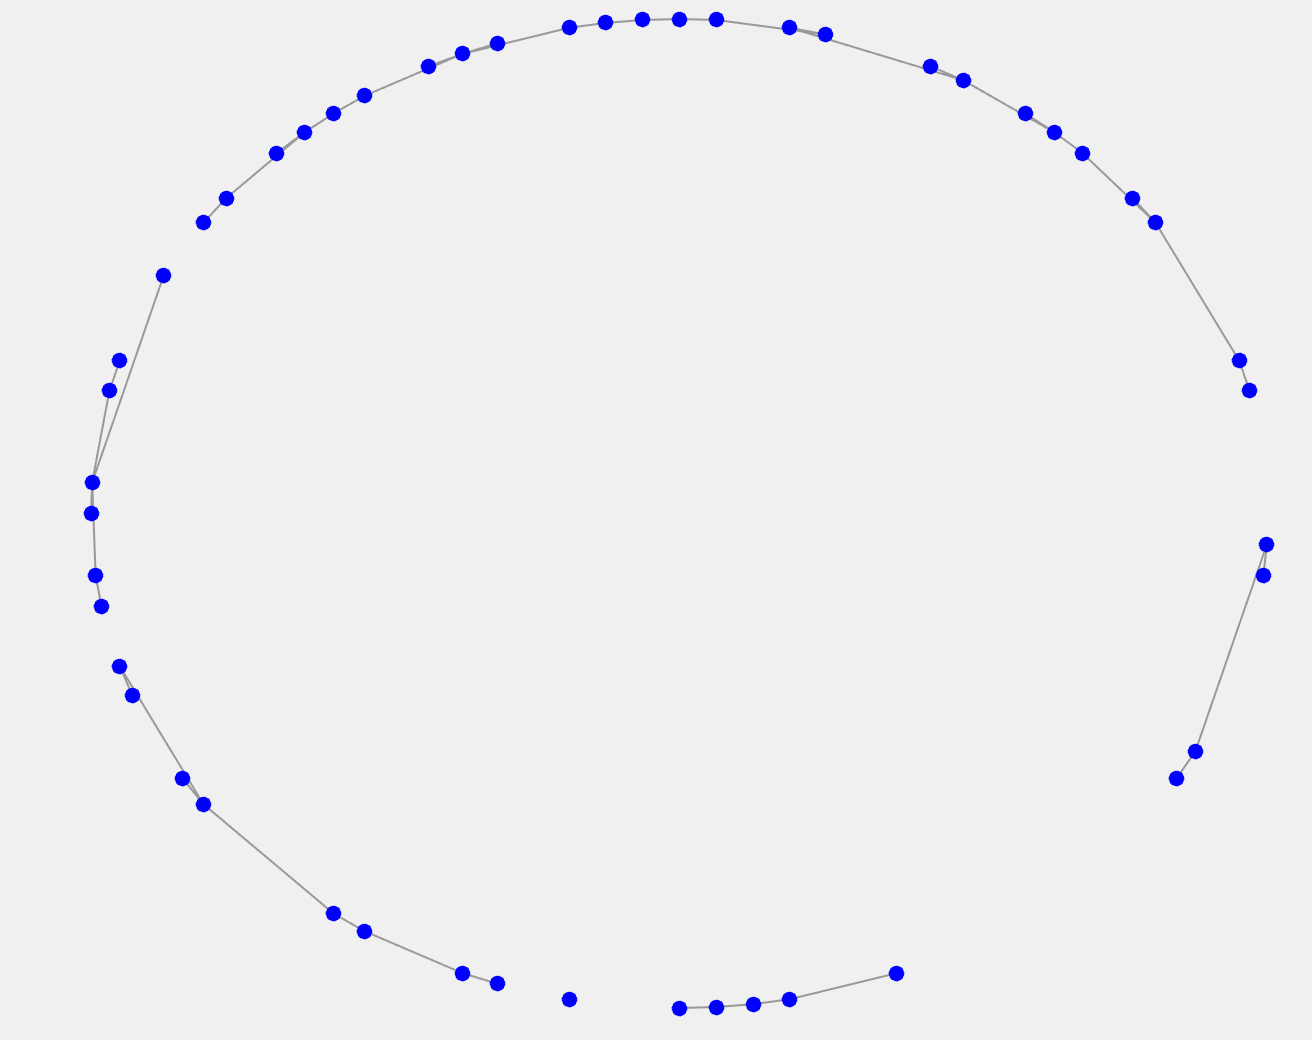
\includegraphics[width = 6cm]{ring_graph/ring_graph_reduced}

\caption{a.original graph b.downsampled graph(red vertices are kept) c. reduced graph}
\end{figure}


The downsampled vertices greatly influence how the reduced graph is rewired. It seems like a disconnection occurs if most of the vertices between the two are eliminated.


With a evenly downsampled graph (every other vertex is kept), can we get better results?  Maybe experiment with different clustering method to get a evenly downsampled graph?

Note: If we perform MMF on the Laplacian matrix, the reduced matrix we get is not a valid graph Laplacian.

\subsection{$A = L$ vs. $A = I - L$}
\begin{itemize}
\item When $A = L$, our weighted adjacency matrix is $W = $ diag(diag($H$)) - $H$. 
\item When $A = I - L$, our Laplacian is $L = I - H$ and our weighted adjacency matrix is $W = $ diag(diag($L$)) - $L$.

\begin{figure}[H]
\centering
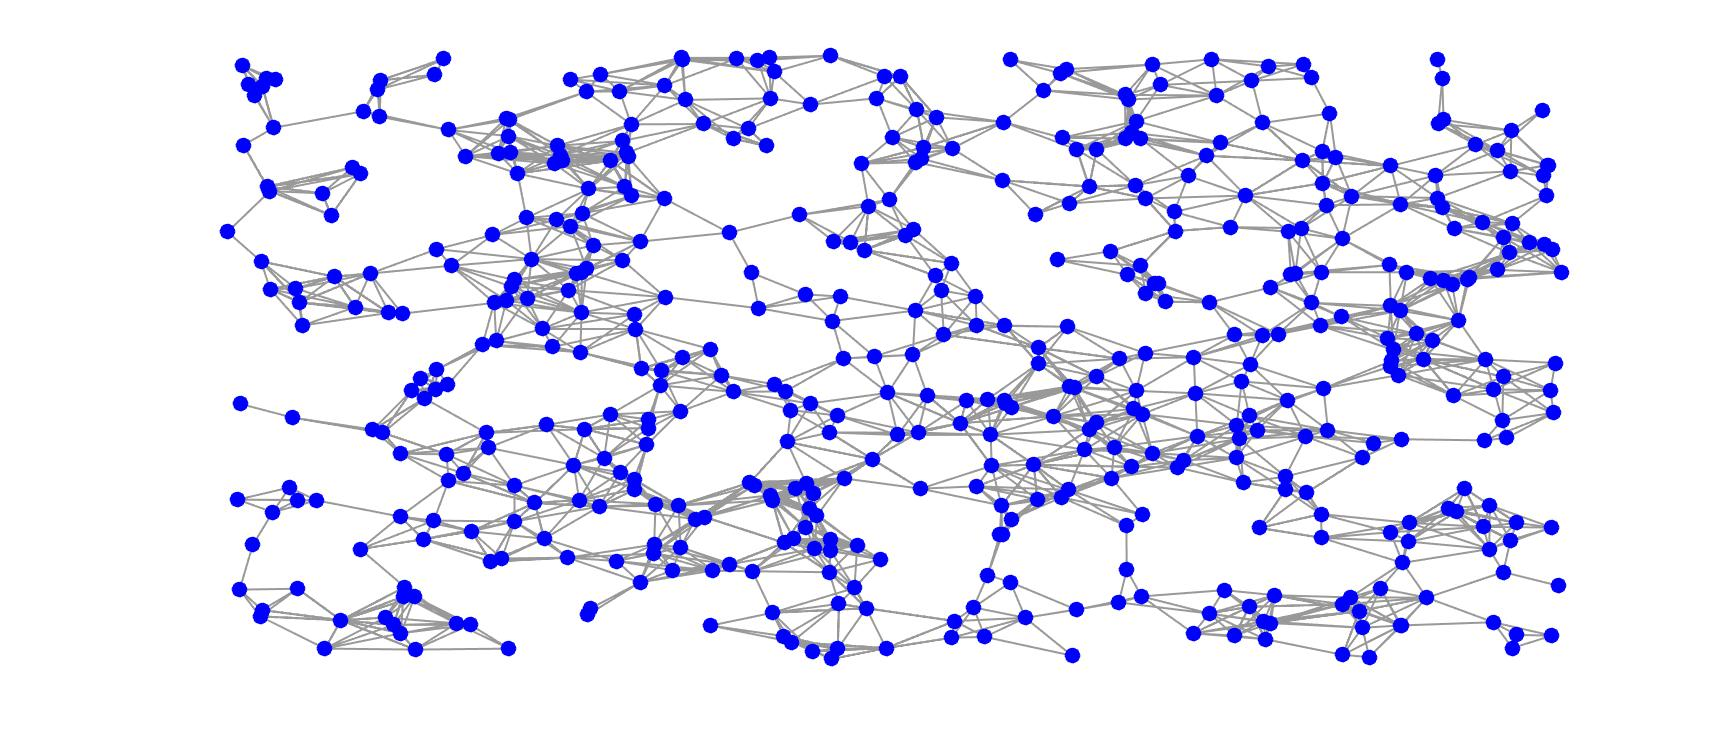
\includegraphics[width = 6 cm]{clusters/original_sensor}
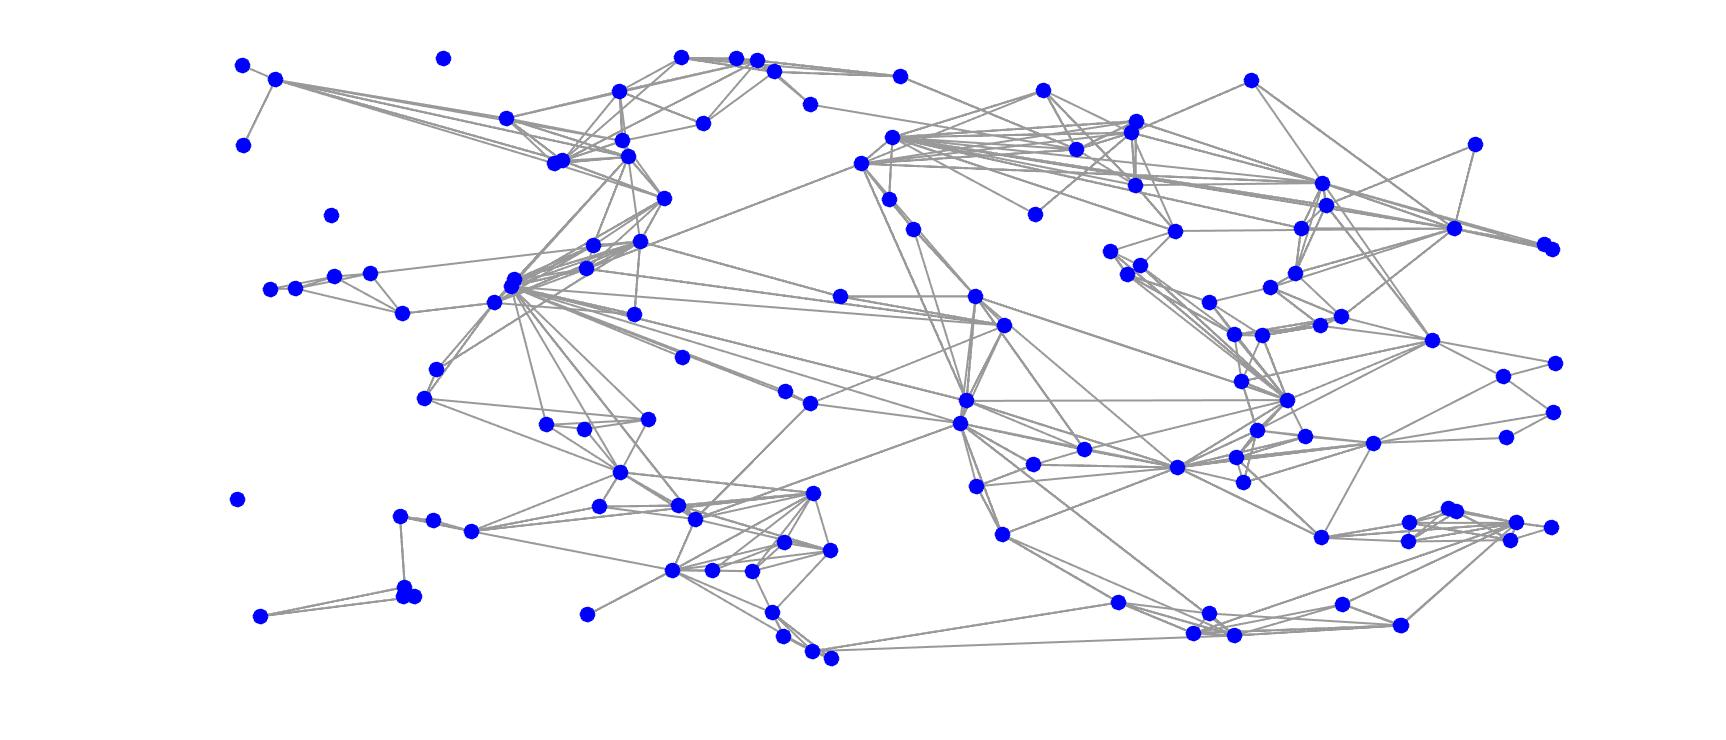
\includegraphics[width = 6 cm]{sensor_network/downsampled_L}
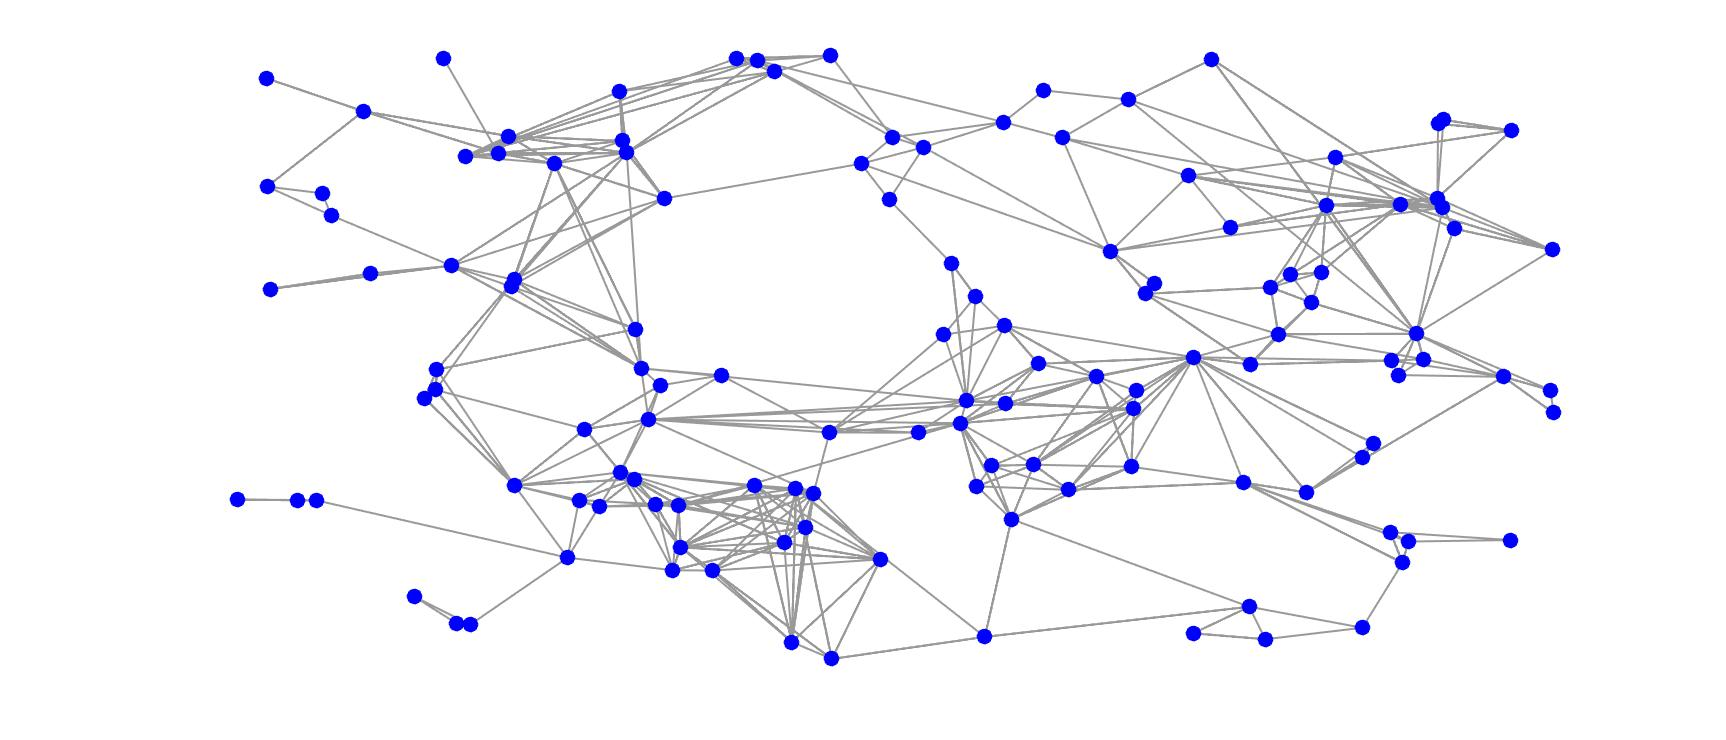
\includegraphics[width = 6 cm]{sensor_network/downsampled_I-L}

\caption{1. Original graph (gsp\_david \_sensor\_network) with 500 vertices. 2. Downsampled graph using $A = L$. 3. Downsampled graph using $A = I - L$.}
\end{figure}
\item The two are very comparable, but it seems like the downsampling using $A = I - L$ captures the sparsity/density of the original graph a bit better.
\end{itemize}

\subsection{Edge Weights}
Compared the proportion of edges with high weight ($> 0.9$) in a gsp\_david\_sensor\_network graph with 500 nodes and the downsampled graph using A = W, A = L, and A = I - L. \\
$22.15\%$  of the edges on the original graph had high weight, and
\begin{itemize}
\item using A = W, $29.28\%$ of the edges had high weight
\item using A = L, $21.82\%$ of the edges had high weight
\item using A = I - L, $22.00\%$ of the edges had high weight
\end{itemize}
When we look at the $n$ highest-weighted edges (however many have weight > 0.9) in the original graph G and the $n \cdot \frac{G downsampled.N}{G.N}$ highest-weighted edges in the downsampled graph, we see that the areas of the downsampled graph which contain high-weighted edges most closely mirror the analogous areas on the original graph when $A = I - L$. $A = W$ does okay, but when $A = L$, the downsampled graph seems to ignore some high-weight areas from the original graph. \\
These judgments are all just visual, so next steps would be to find a way to quantify high-weight edge retention numerically.

\section{Plot Reduced Laplacian Eigenvectors}

Parameters:
\begin{itemize}
\item G: gsp\_david\_sensor\_network
\item 2 stages
\item 1 cluster
\end{itemize}

\begin{figure}[H]
\centering
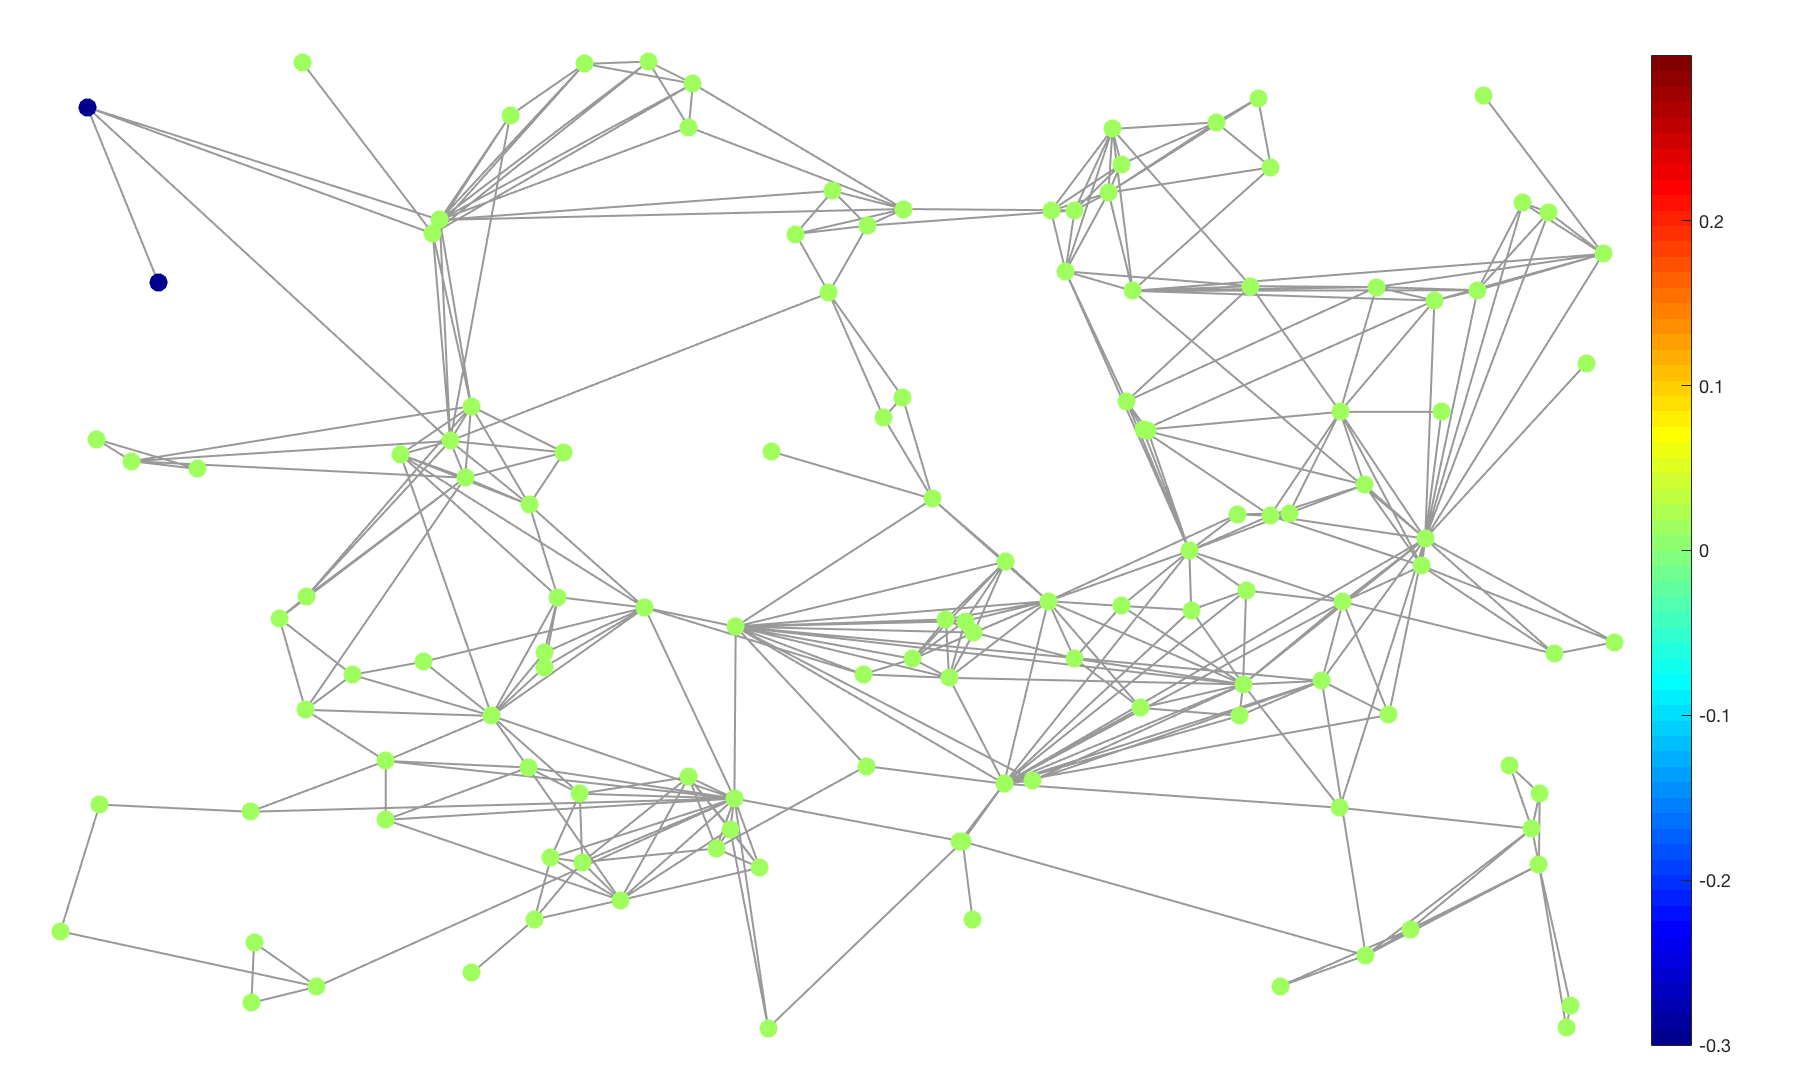
\includegraphics[width = 7cm]{plot_eigenvectors/reduced_eigenvec_1}
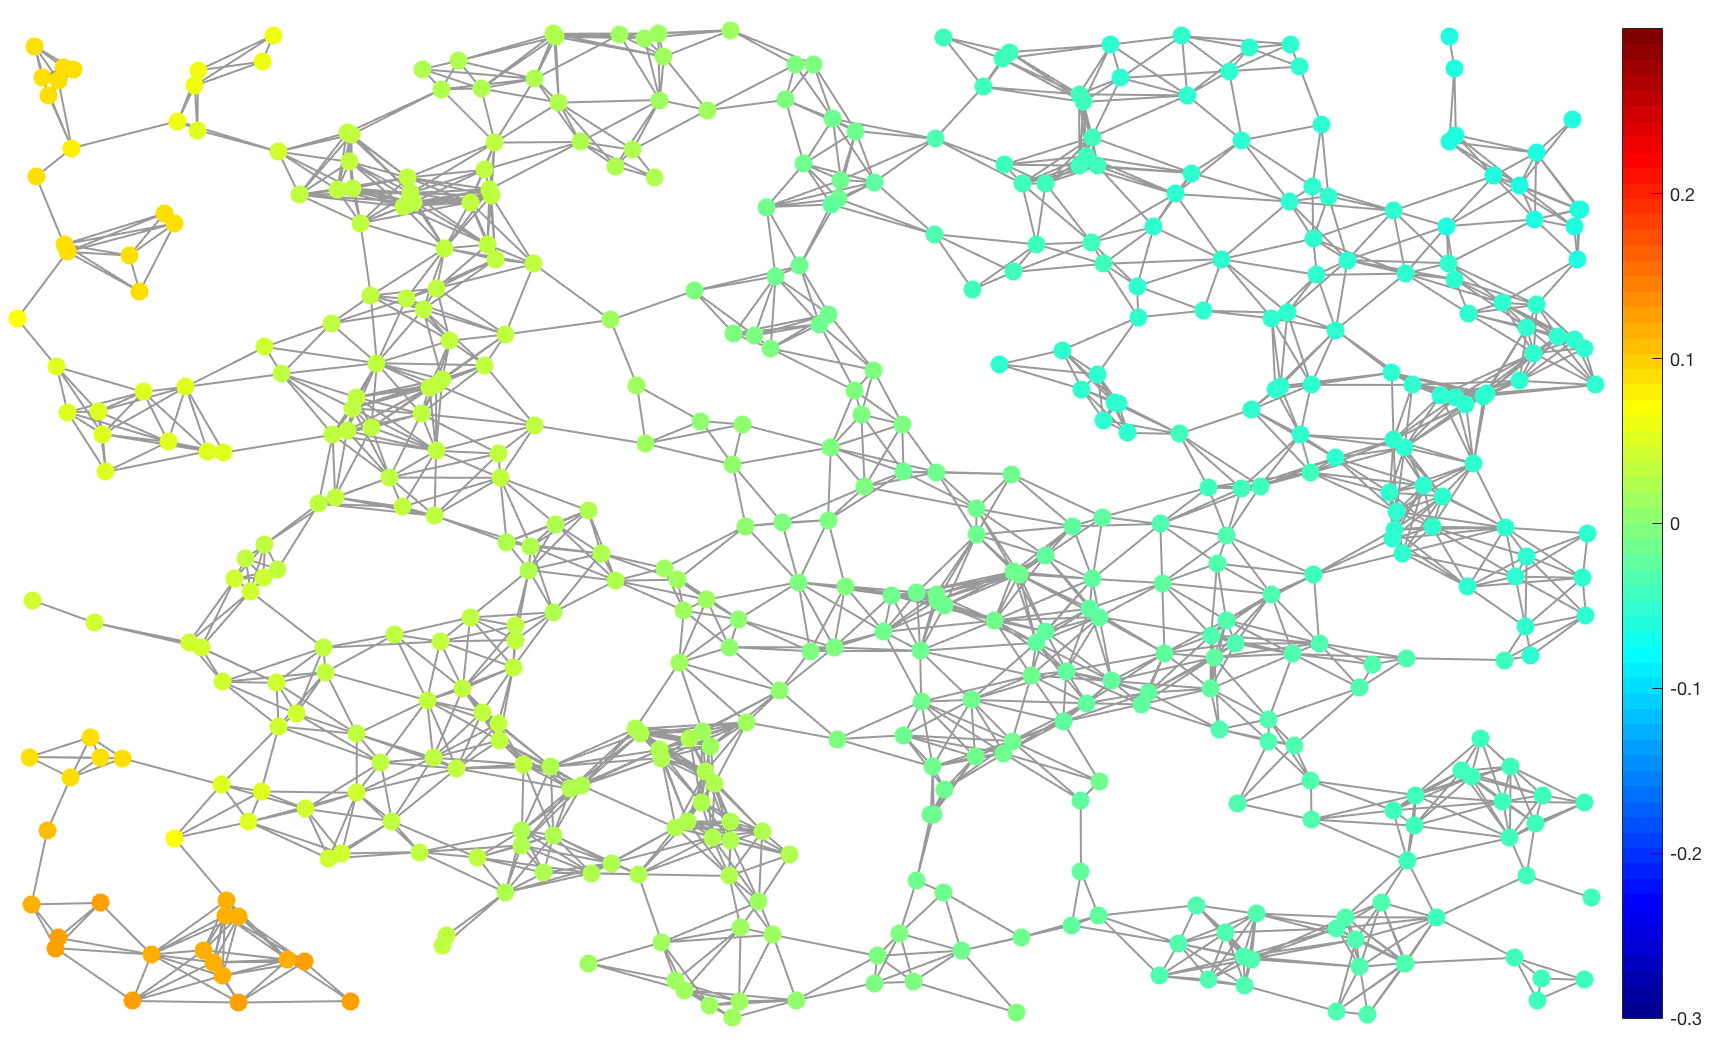
\includegraphics[width = 7cm]{plot_eigenvectors/original_eigenvec_1}

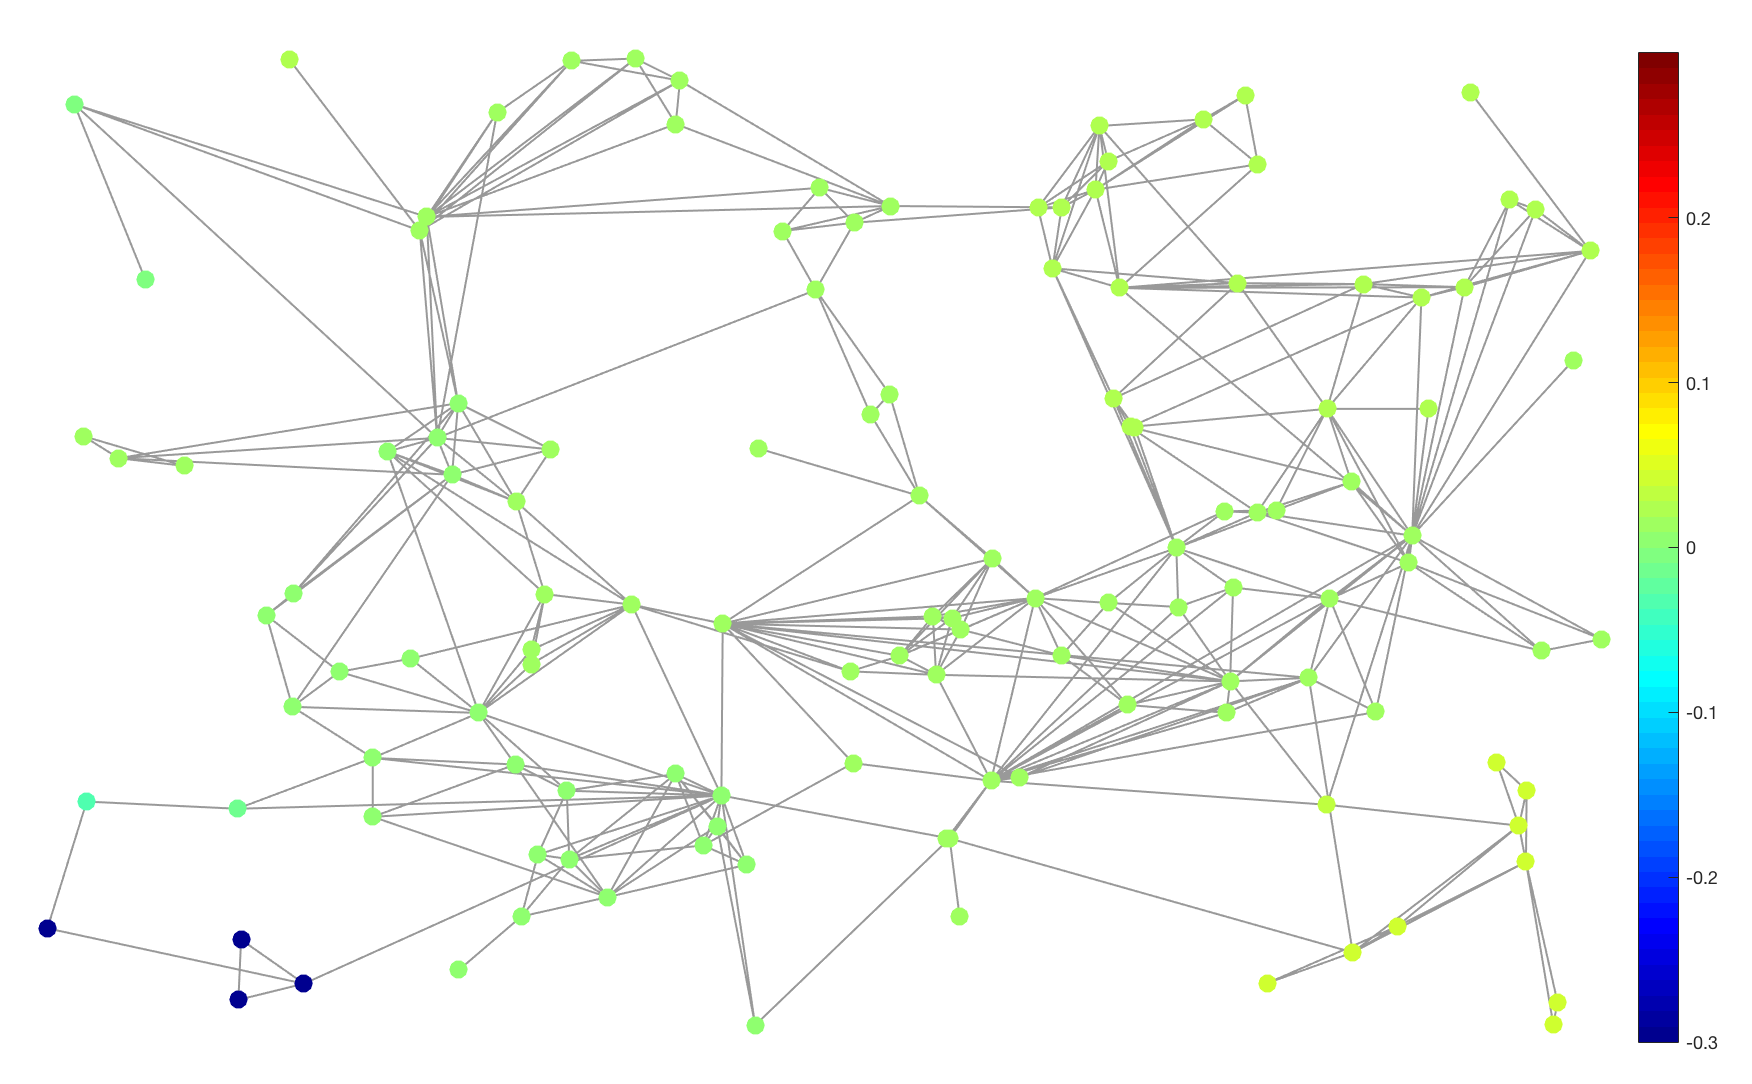
\includegraphics[width = 7cm]{plot_eigenvectors/reduced_eigenvec_2}
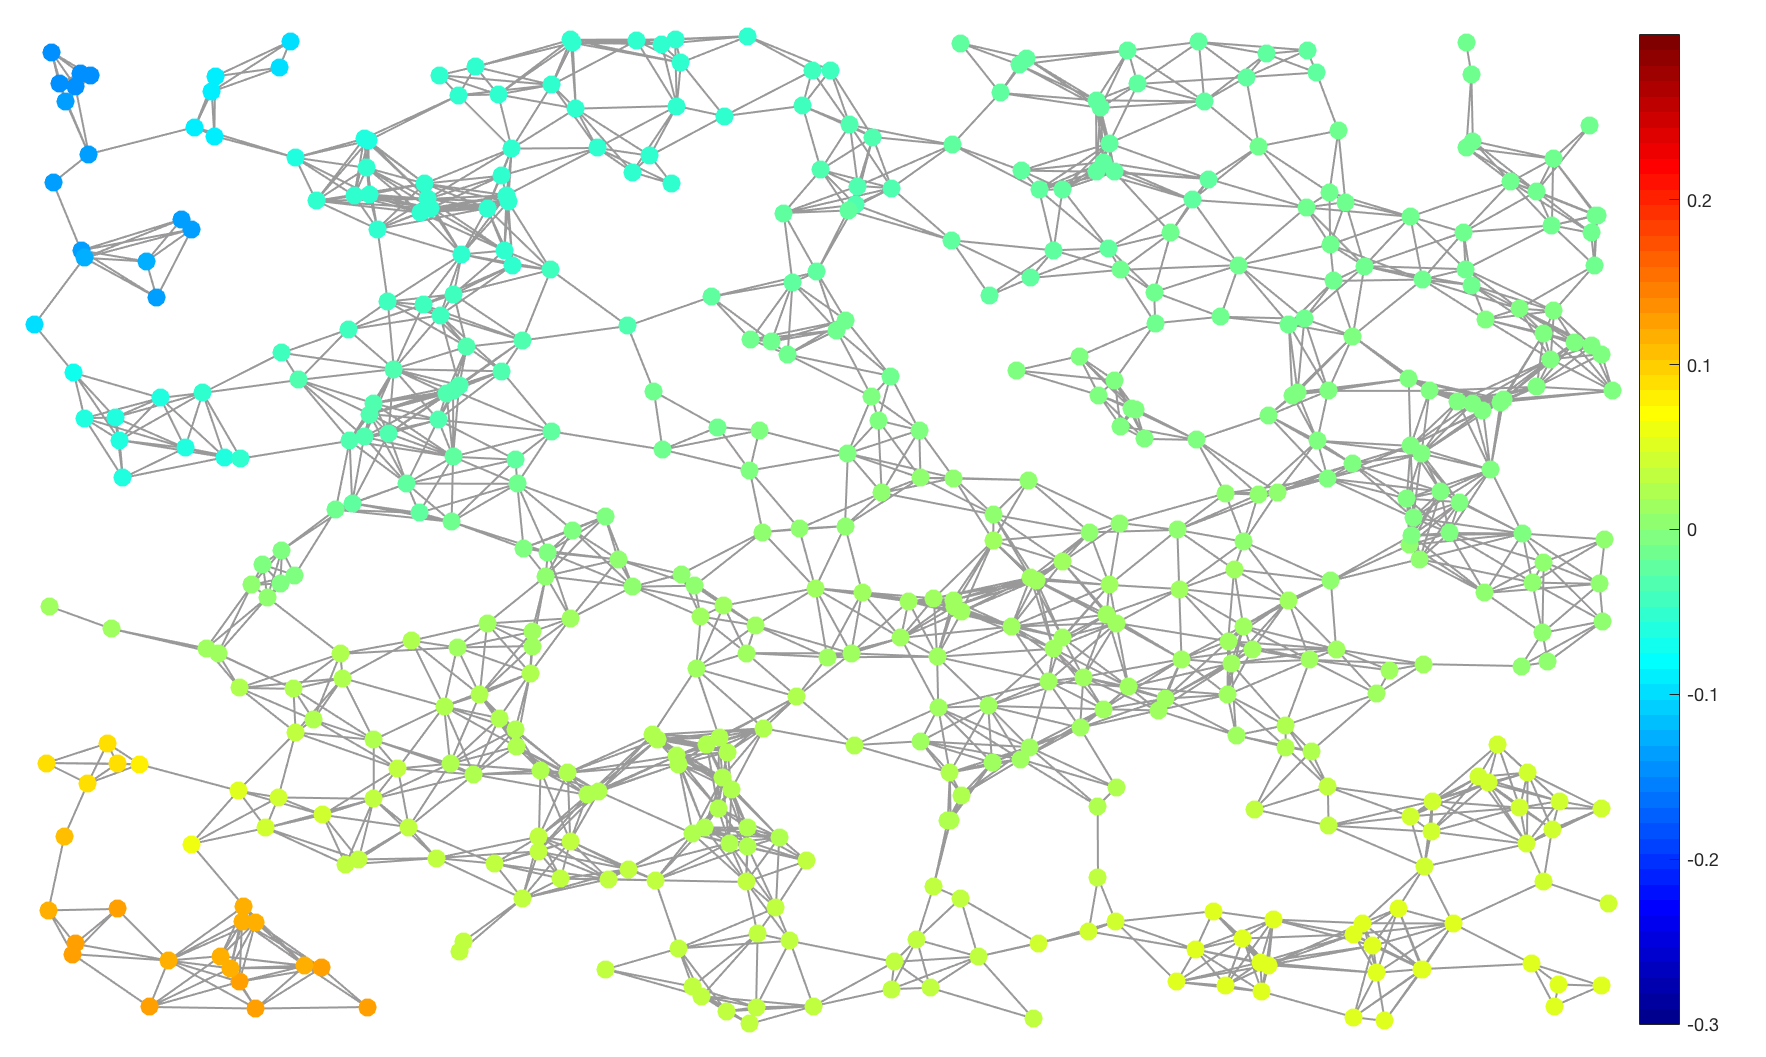
\includegraphics[width = 7cm]{plot_eigenvectors/original_eigenvec_2}

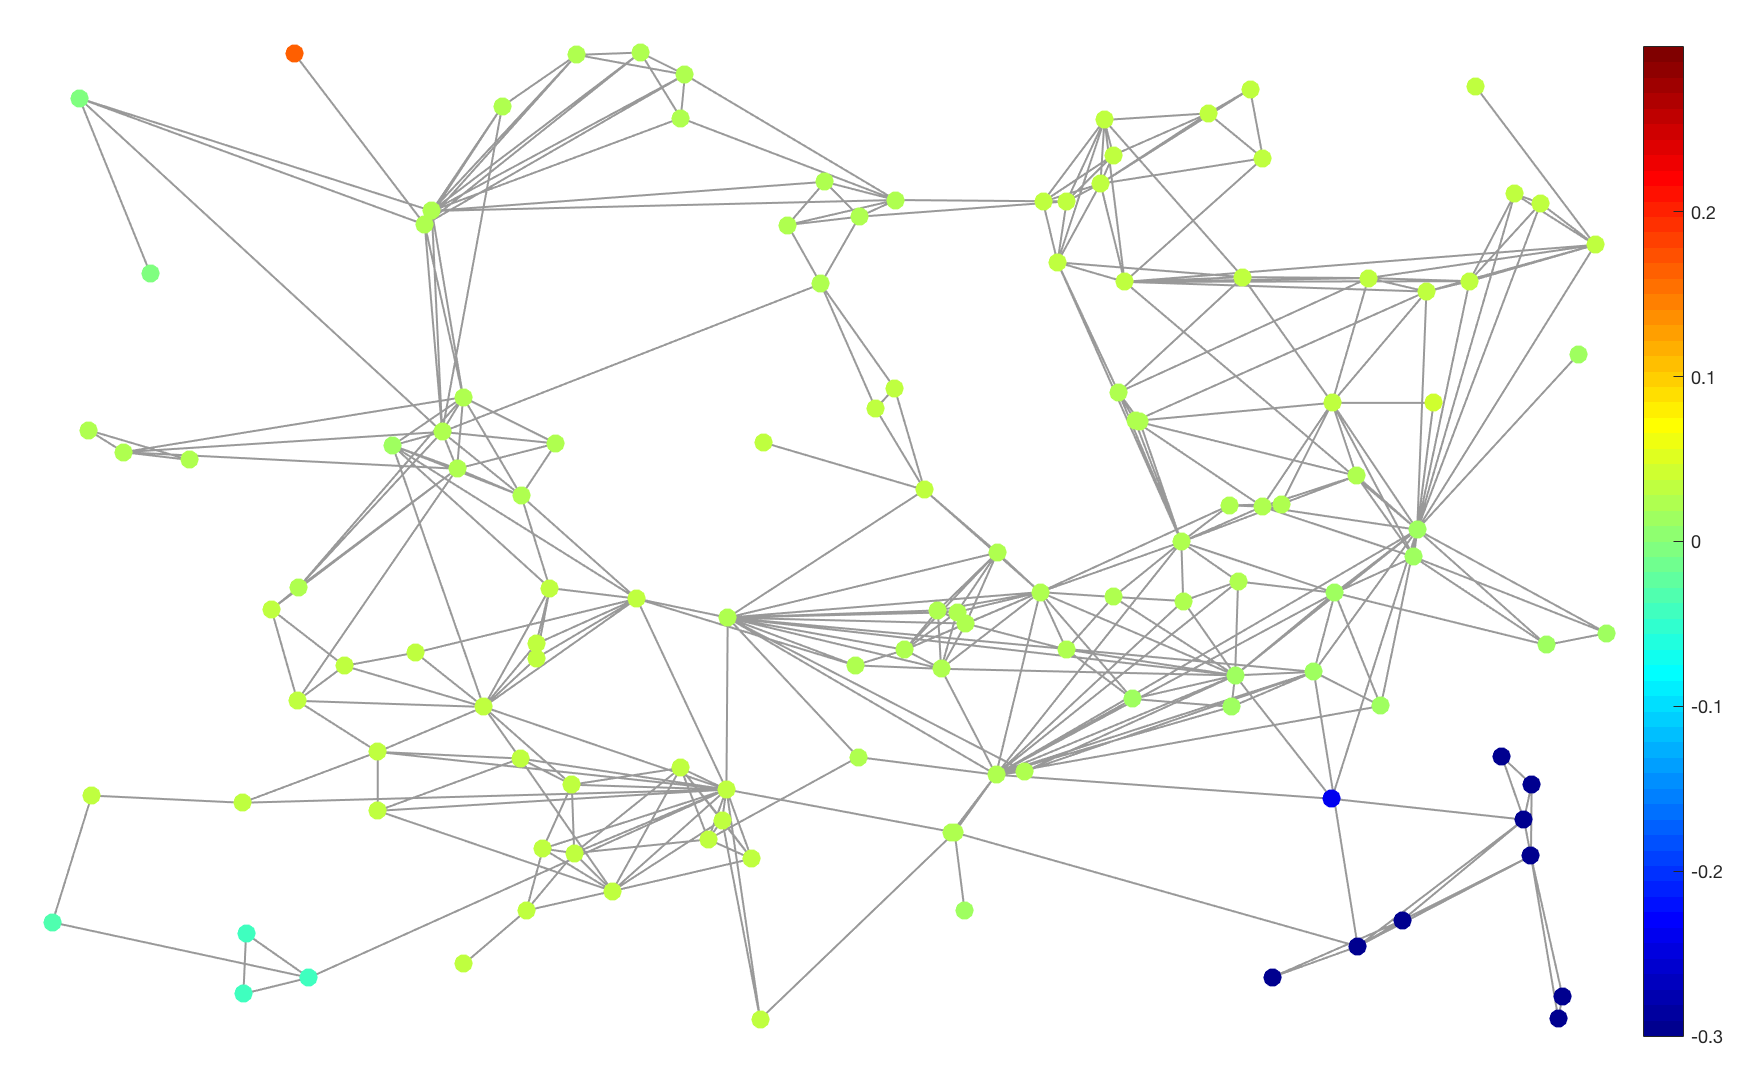
\includegraphics[width = 7cm]{plot_eigenvectors/reduced_eigenvec_3}
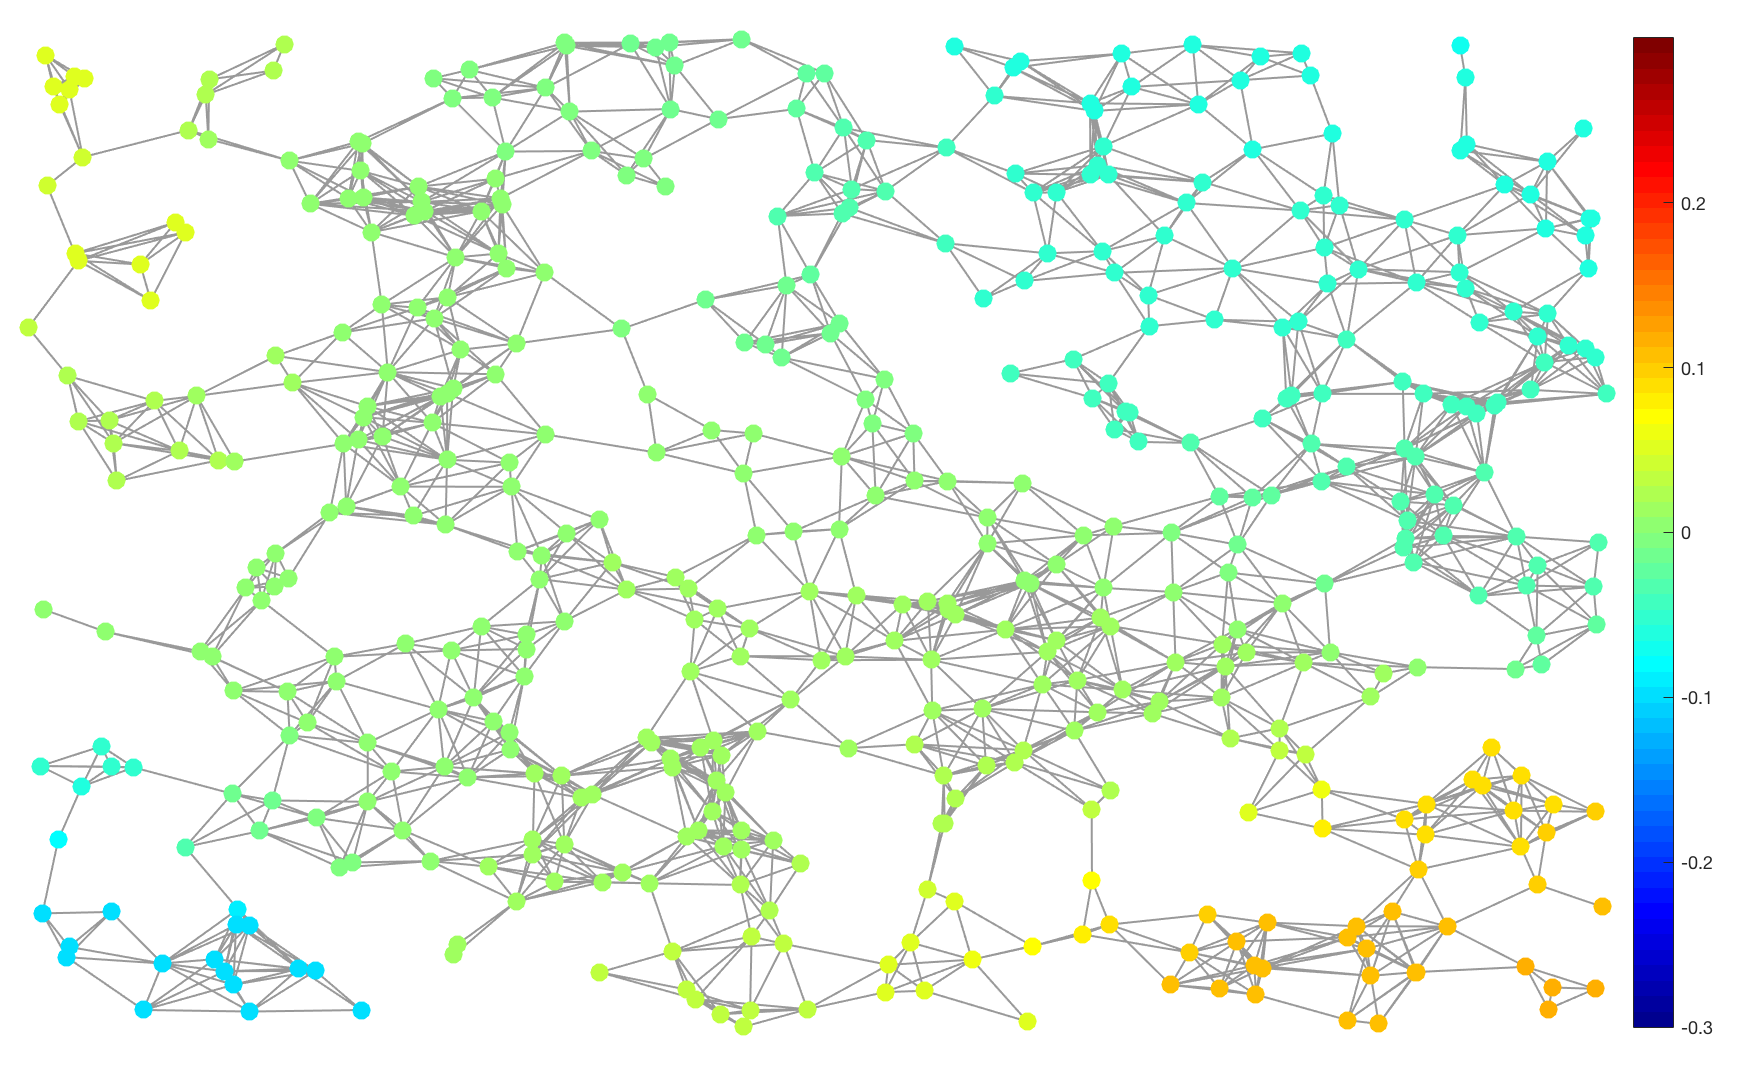
\includegraphics[width = 7cm]{plot_eigenvectors/original_eigenvec_3}

\caption{The left column shows the 2nd, 3rd and 4th eigenvectors of the reduced graph Laplacian. The right column shows the 2nd, 3rd and 4th smallest eigenvectors of the original graph Laplacian.}

\end{figure}

\section{Interpolation}

The adjacency matrix of the reduced graph is obtained from $H-Diag(H)$. Then we interpolate the eigenvectors of the reduced graph Laplacian and compare them to the eigenvectors of the original graph Laplacian.

\begin{figure}[H]
\centering
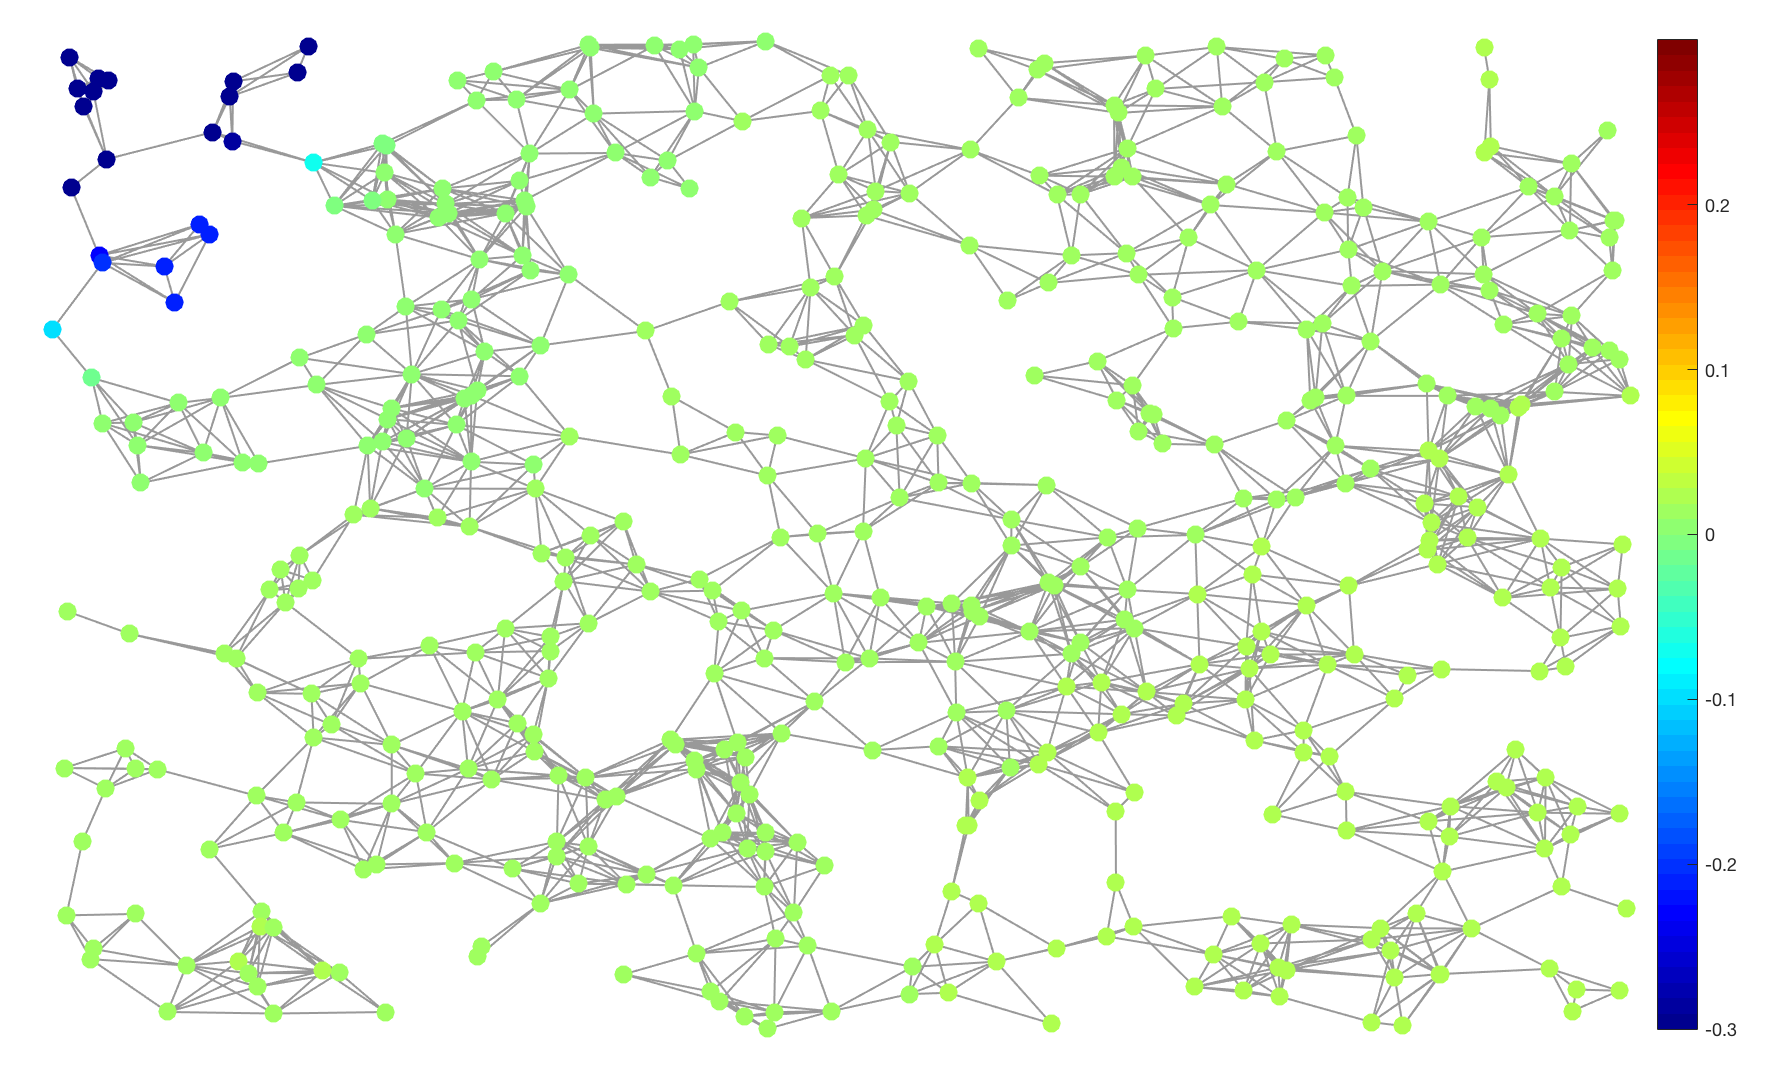
\includegraphics[width = 7cm]{interpolation/interpolate_2nd_eigen}
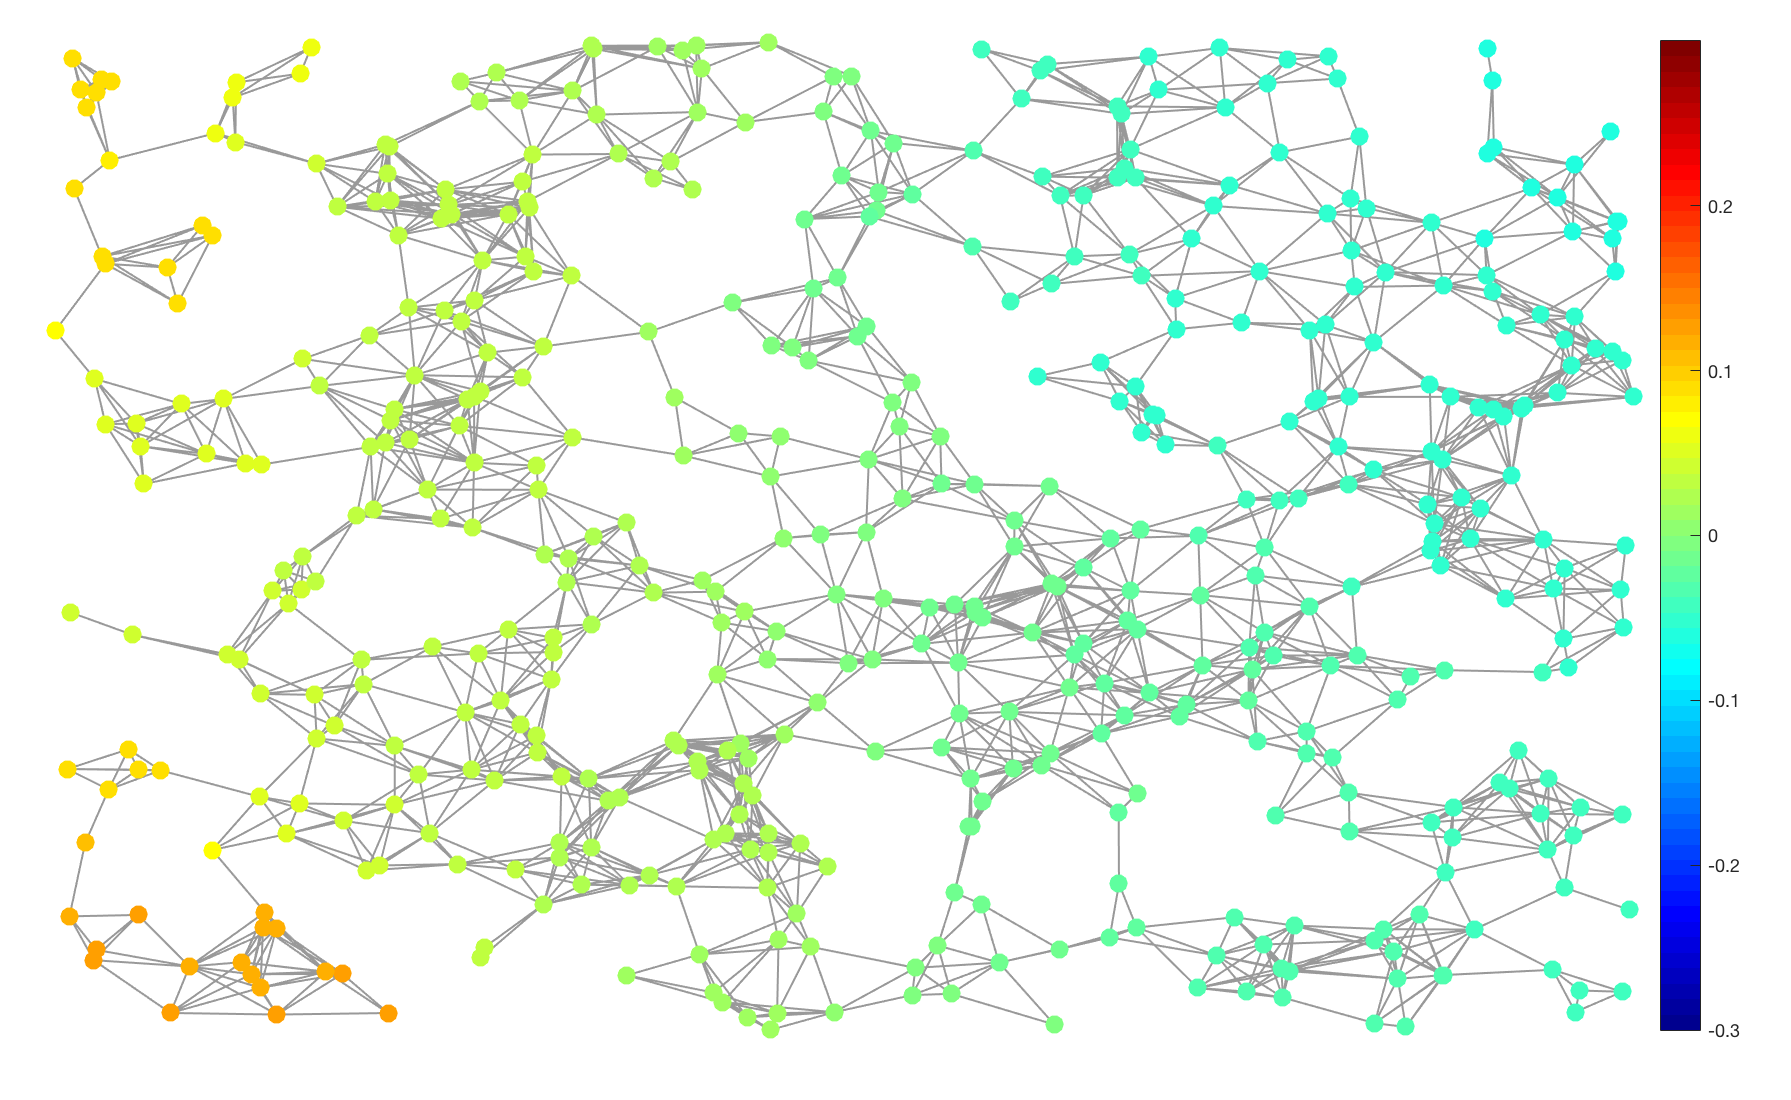
\includegraphics[width = 7cm]{interpolation/original_2nd_eigen}

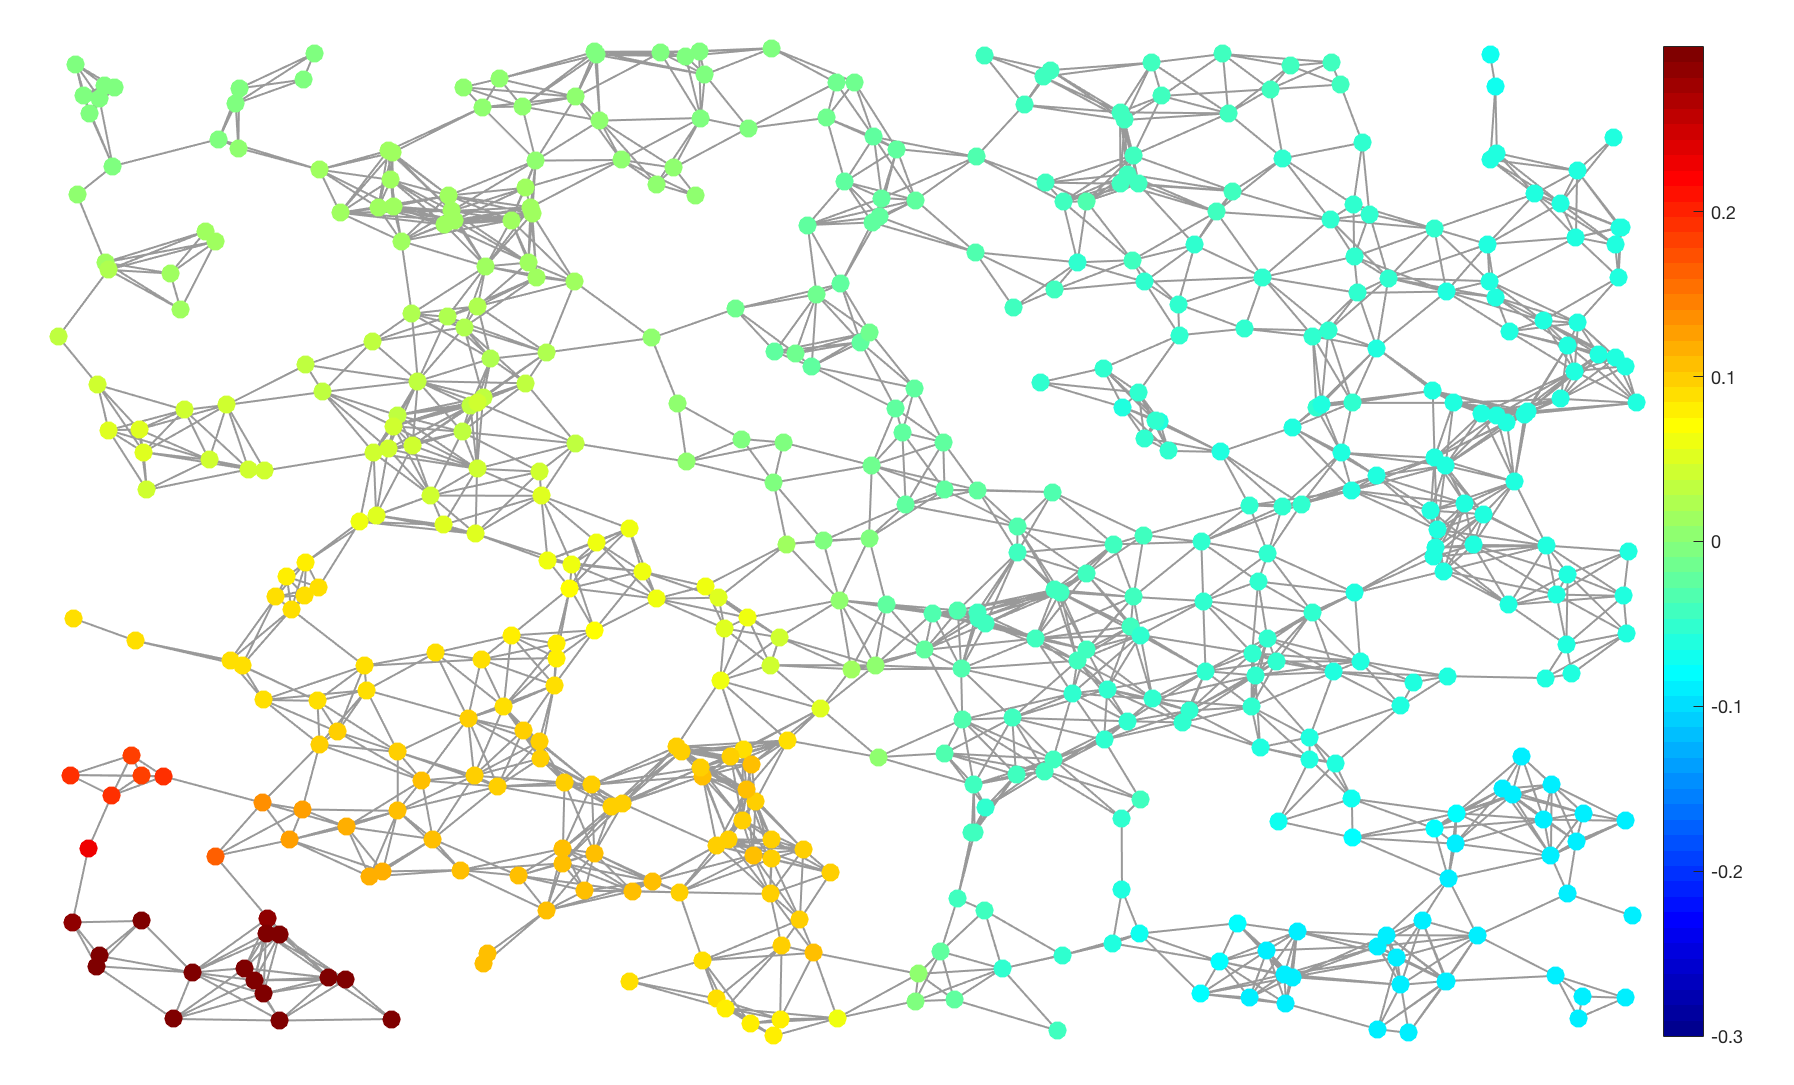
\includegraphics[width = 7cm]{interpolation/interpolate_3rd_eigen}
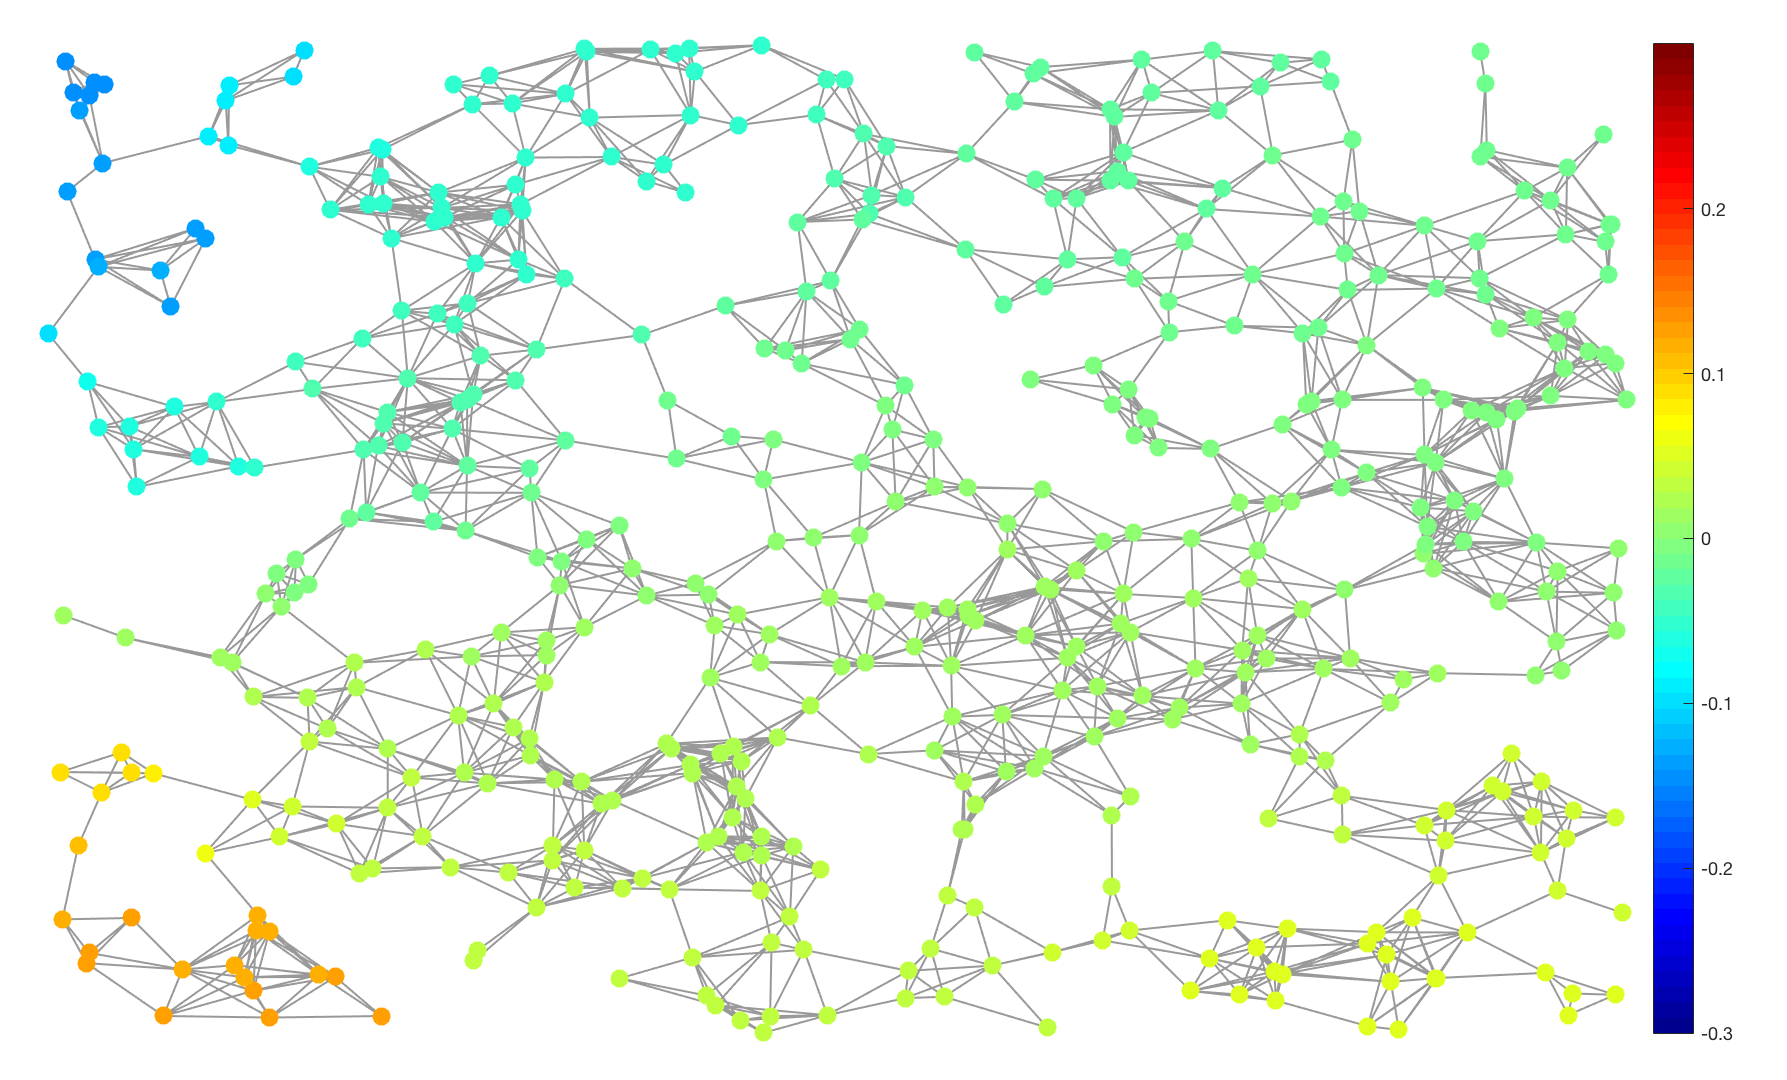
\includegraphics[width = 7cm]{interpolation/original_3rd_eigen}

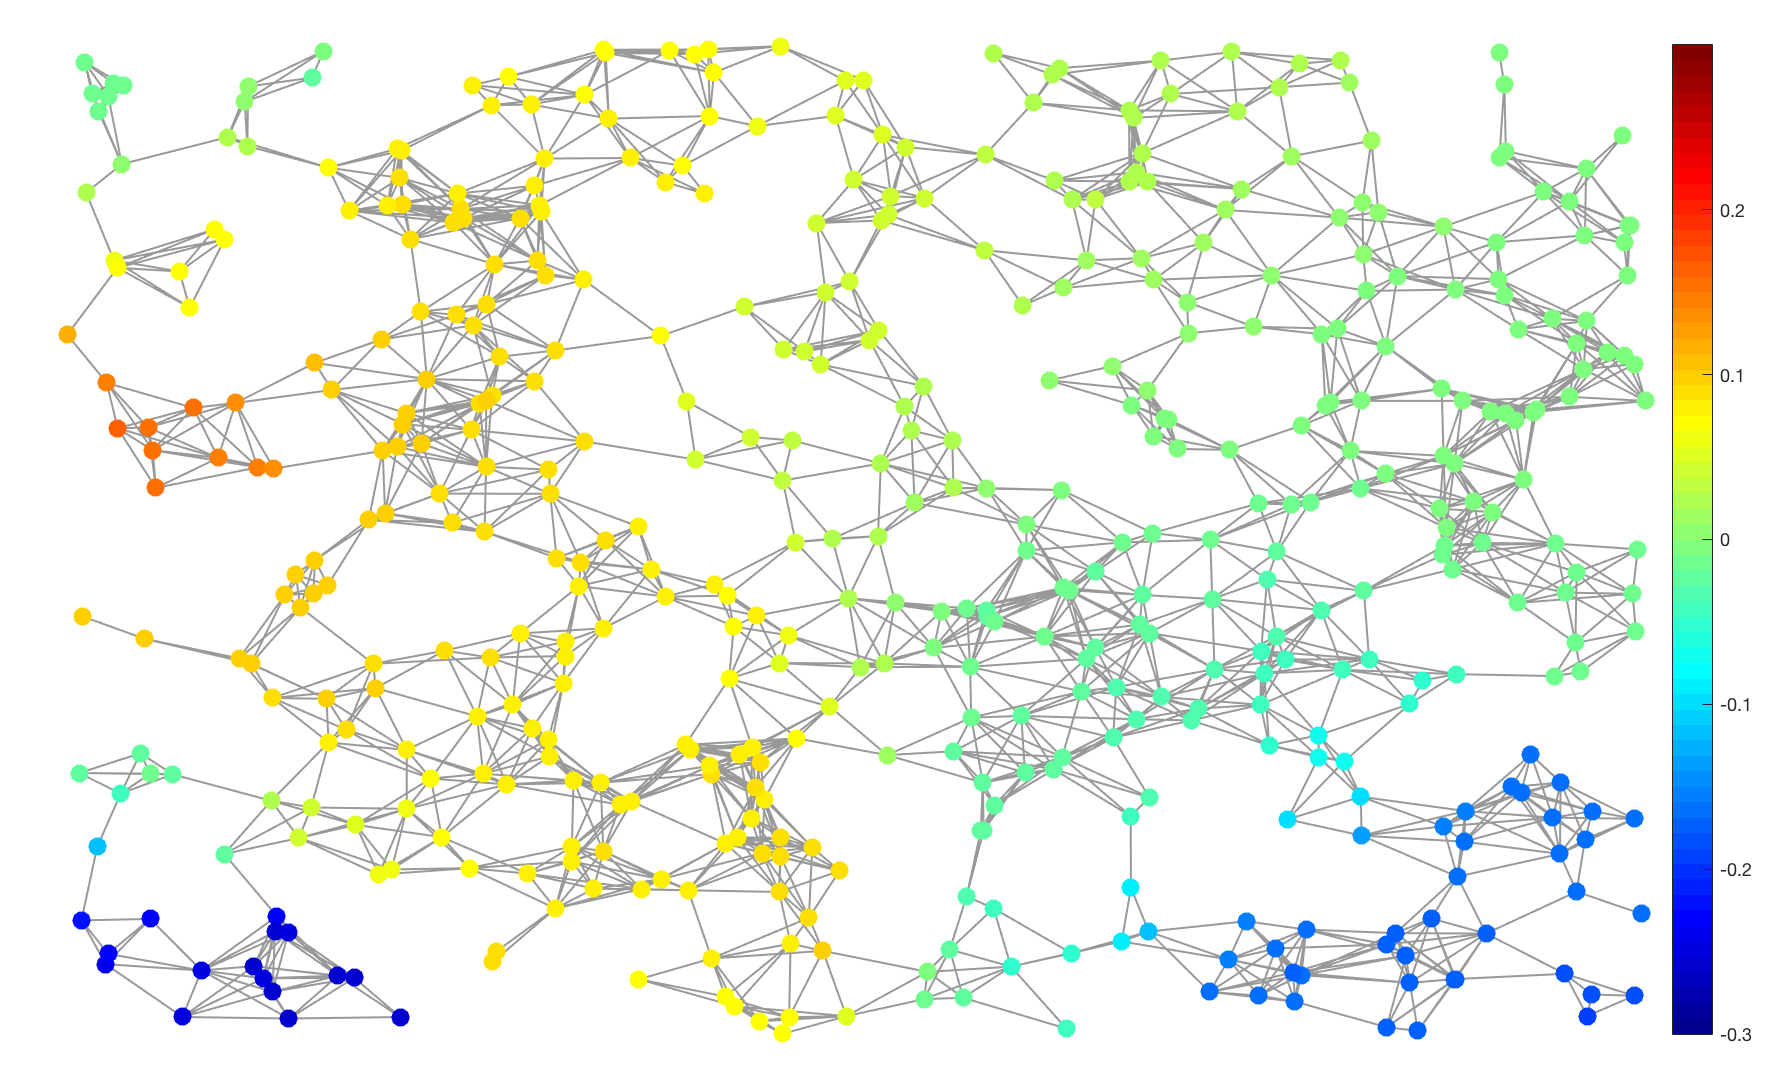
\includegraphics[width = 7cm]{interpolation/interpolate_4th_eigen}
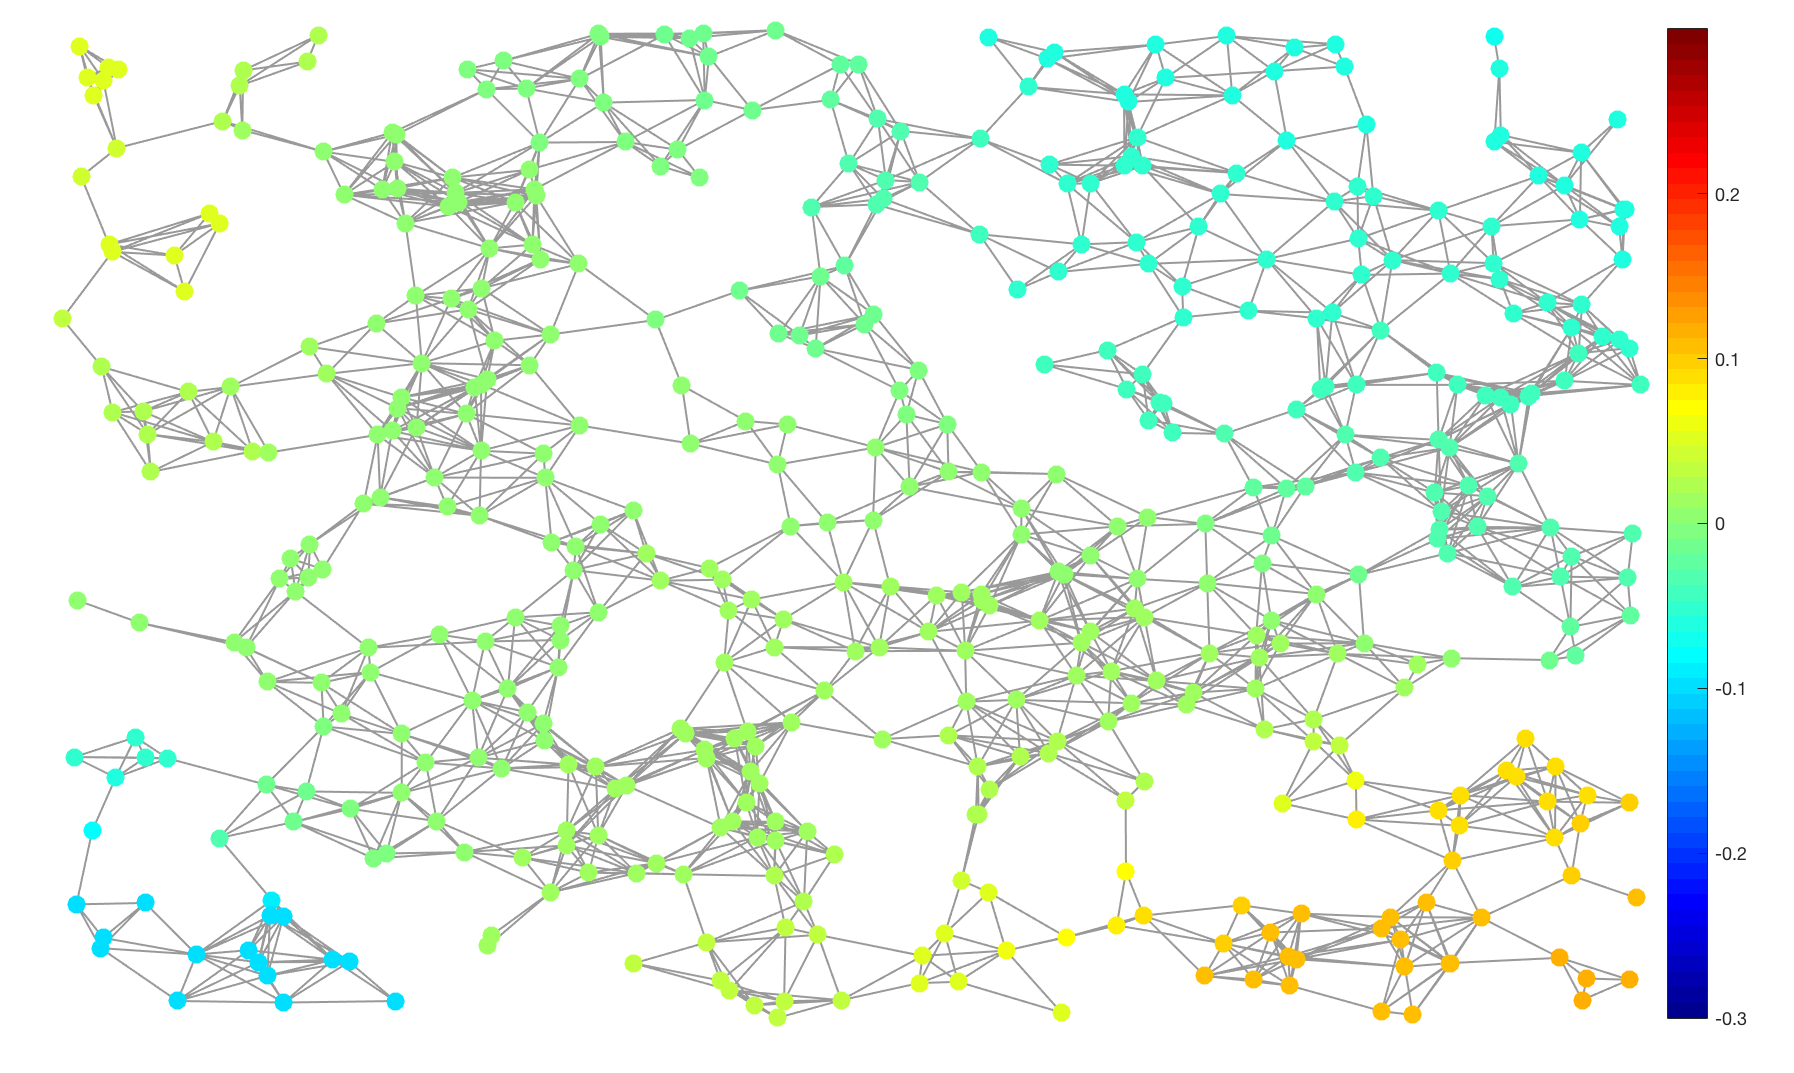
\includegraphics[width = 7cm]{interpolation/original_4th_eigen}

\caption{The left column shows interpolations of the 2nd, 3rd and 4th smallest eigenvectors. The right column shows the 2nd, 3rd and 4th smallest eigenvectors of the original graph}


\end{figure}

\subsection{Interpolation Coefficient Matrix}
Take A as the the weighted adjacency matrix, we notice that the reduced matrix has non-zero diagonals. In this section, we zero out the diagonals at each stage. Also, we set the compression ratio $\mu = 0.2$. Smaller compression ratio seems to give better interpolation results.

First example is on the path graph. Parameters:
\begin{enumerate}
\item 128 vertices
\item compression ratio $\mu = 0.2$
\item 4 stages
\item 2 cluster
\end{enumerate}


\begin{figure}[H]
\centering
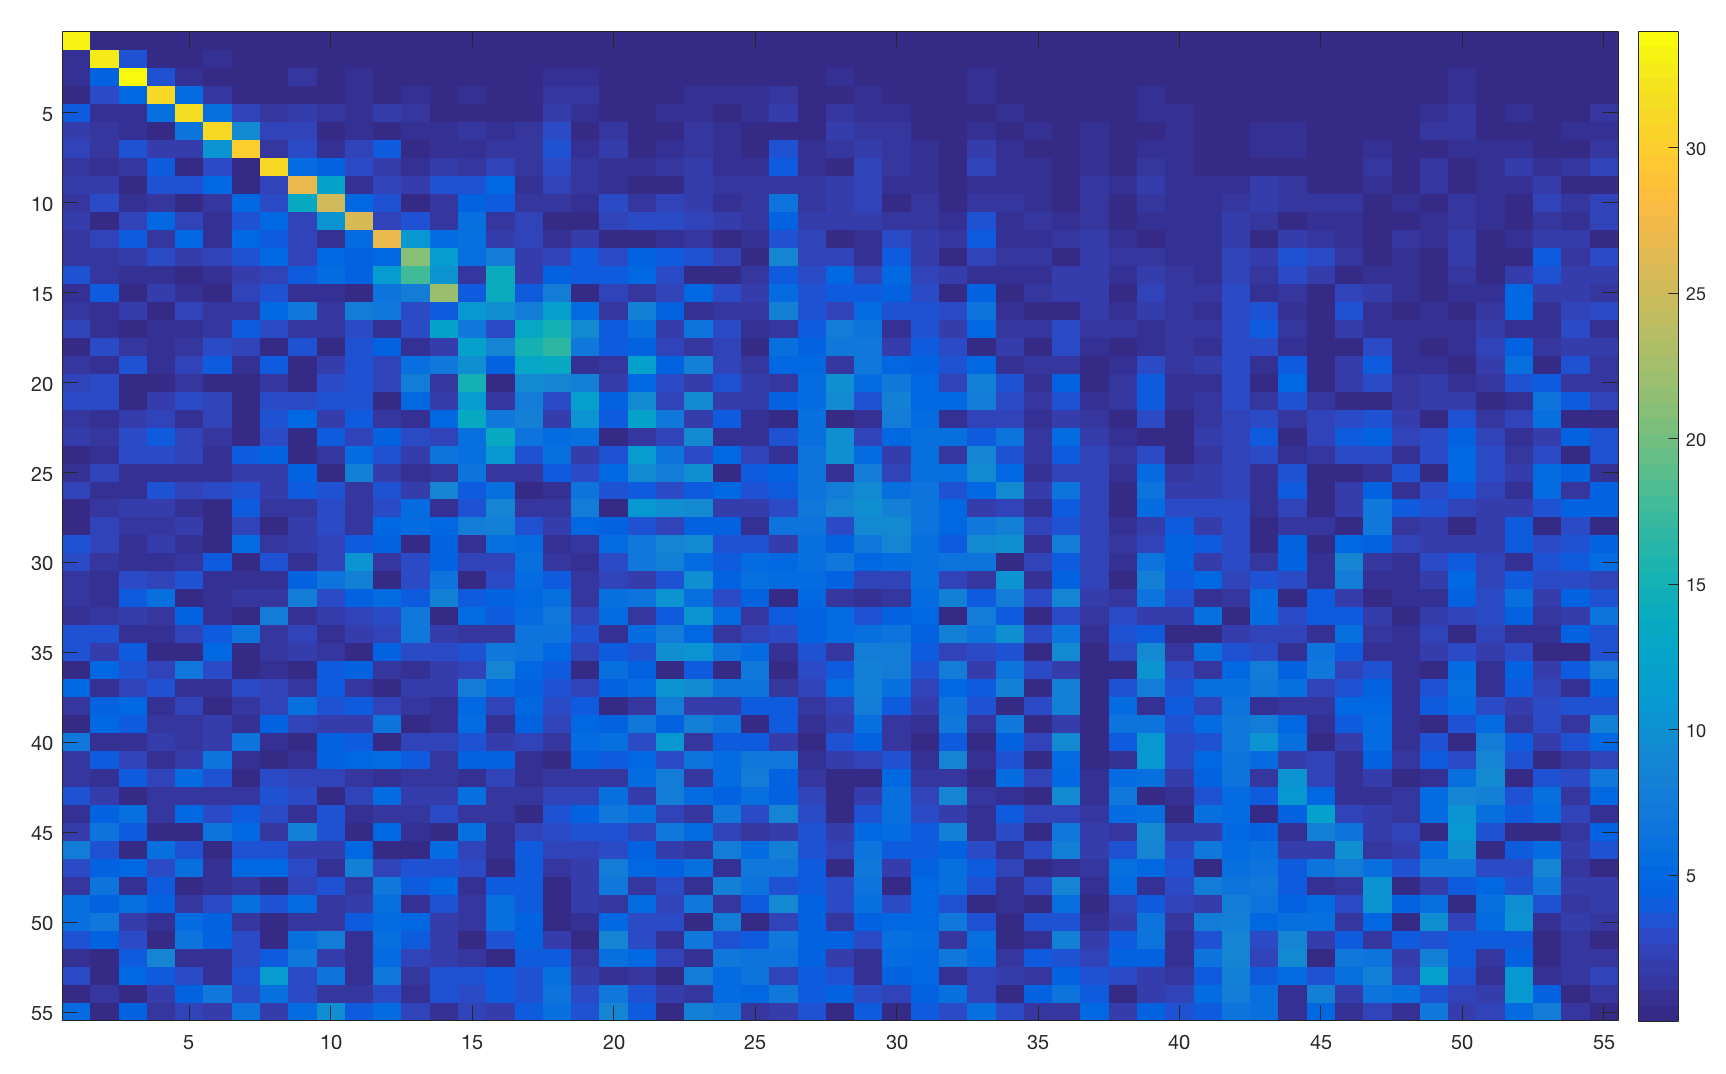
\includegraphics[width = 7 cm]{0629/coefficients_path_graph_4_stages}
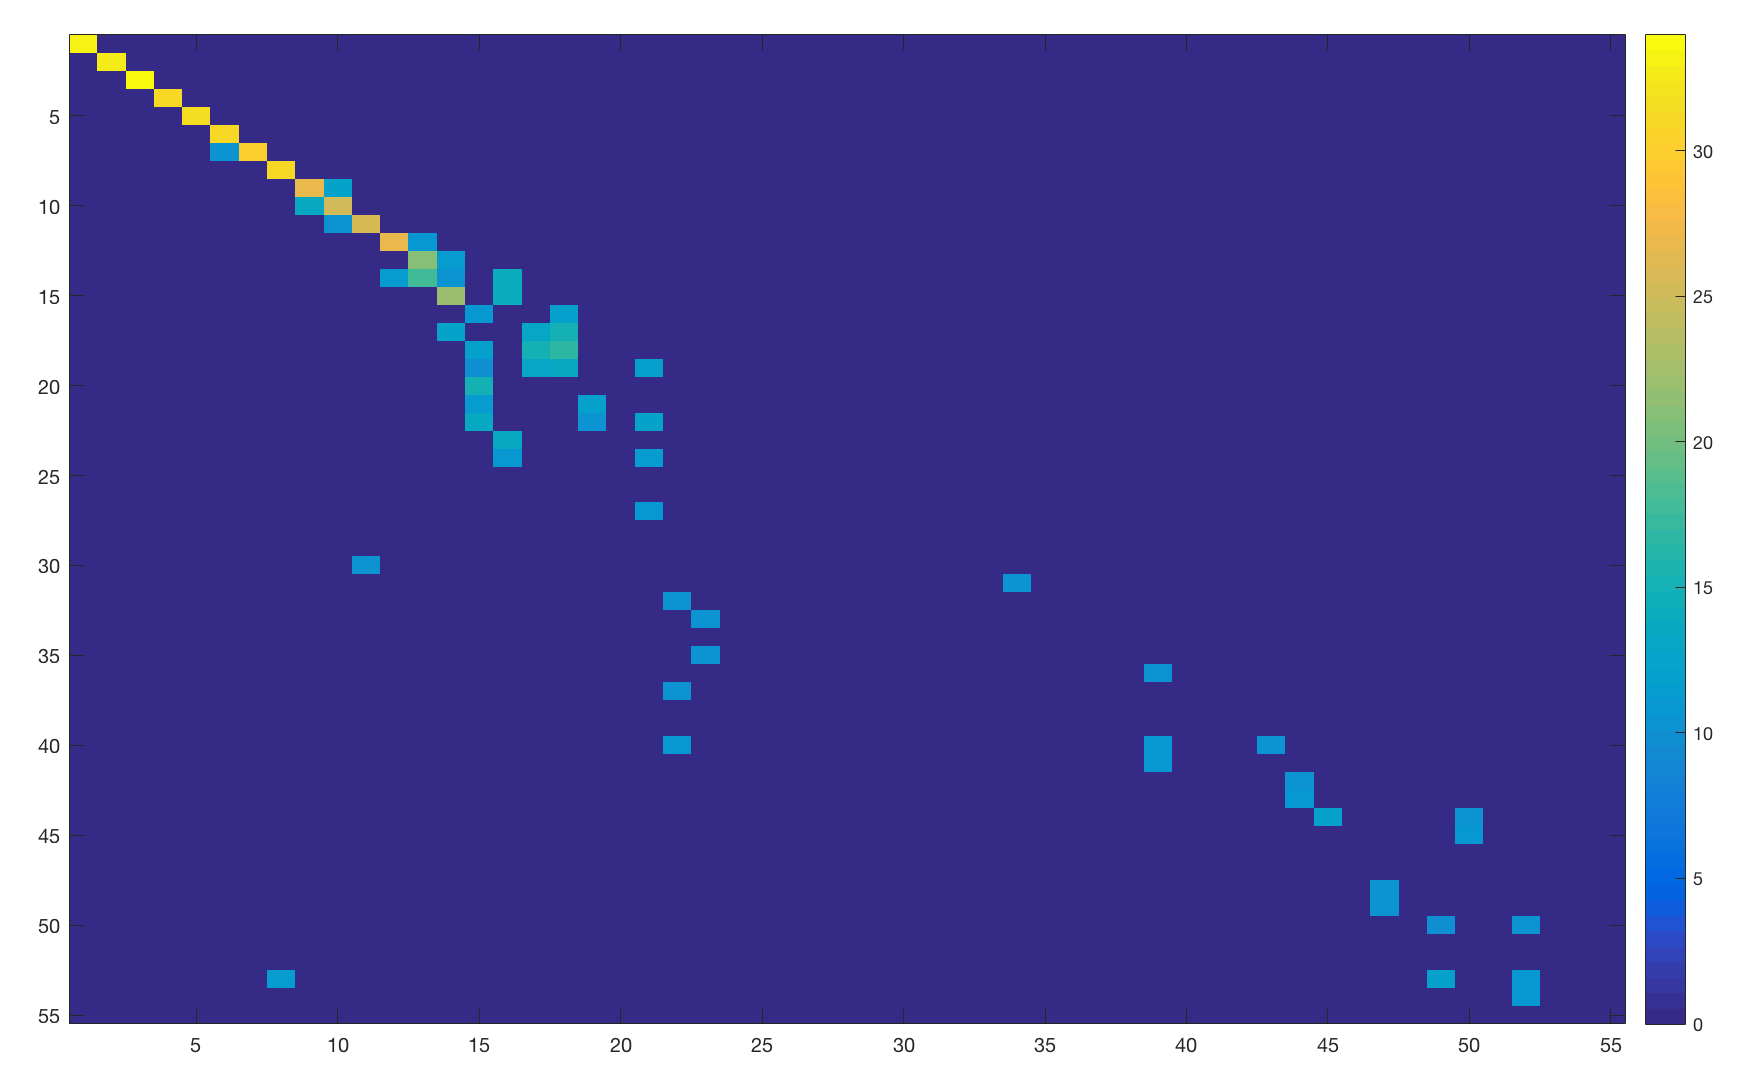
\includegraphics[width = 7 cm]{0629/coefficients_path_graph_4_stages_threshold}

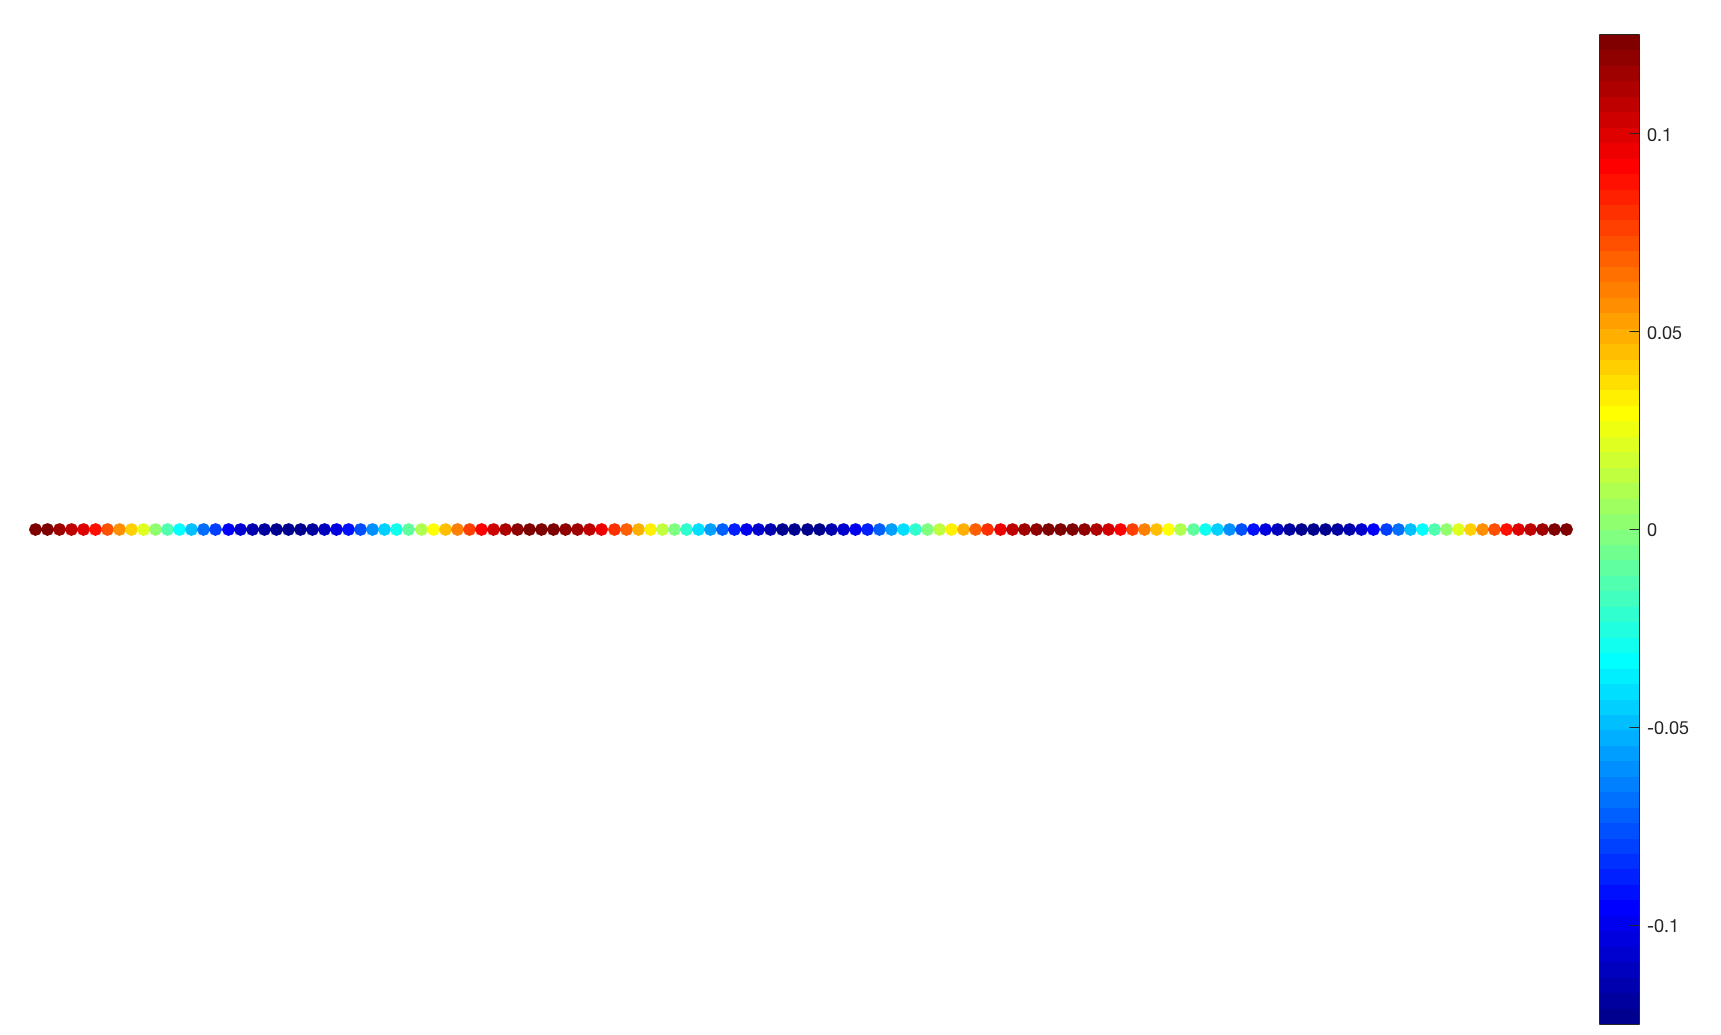
\includegraphics[width = 7cm]{0629/path_graph_4_stages_7th_eigenvec}
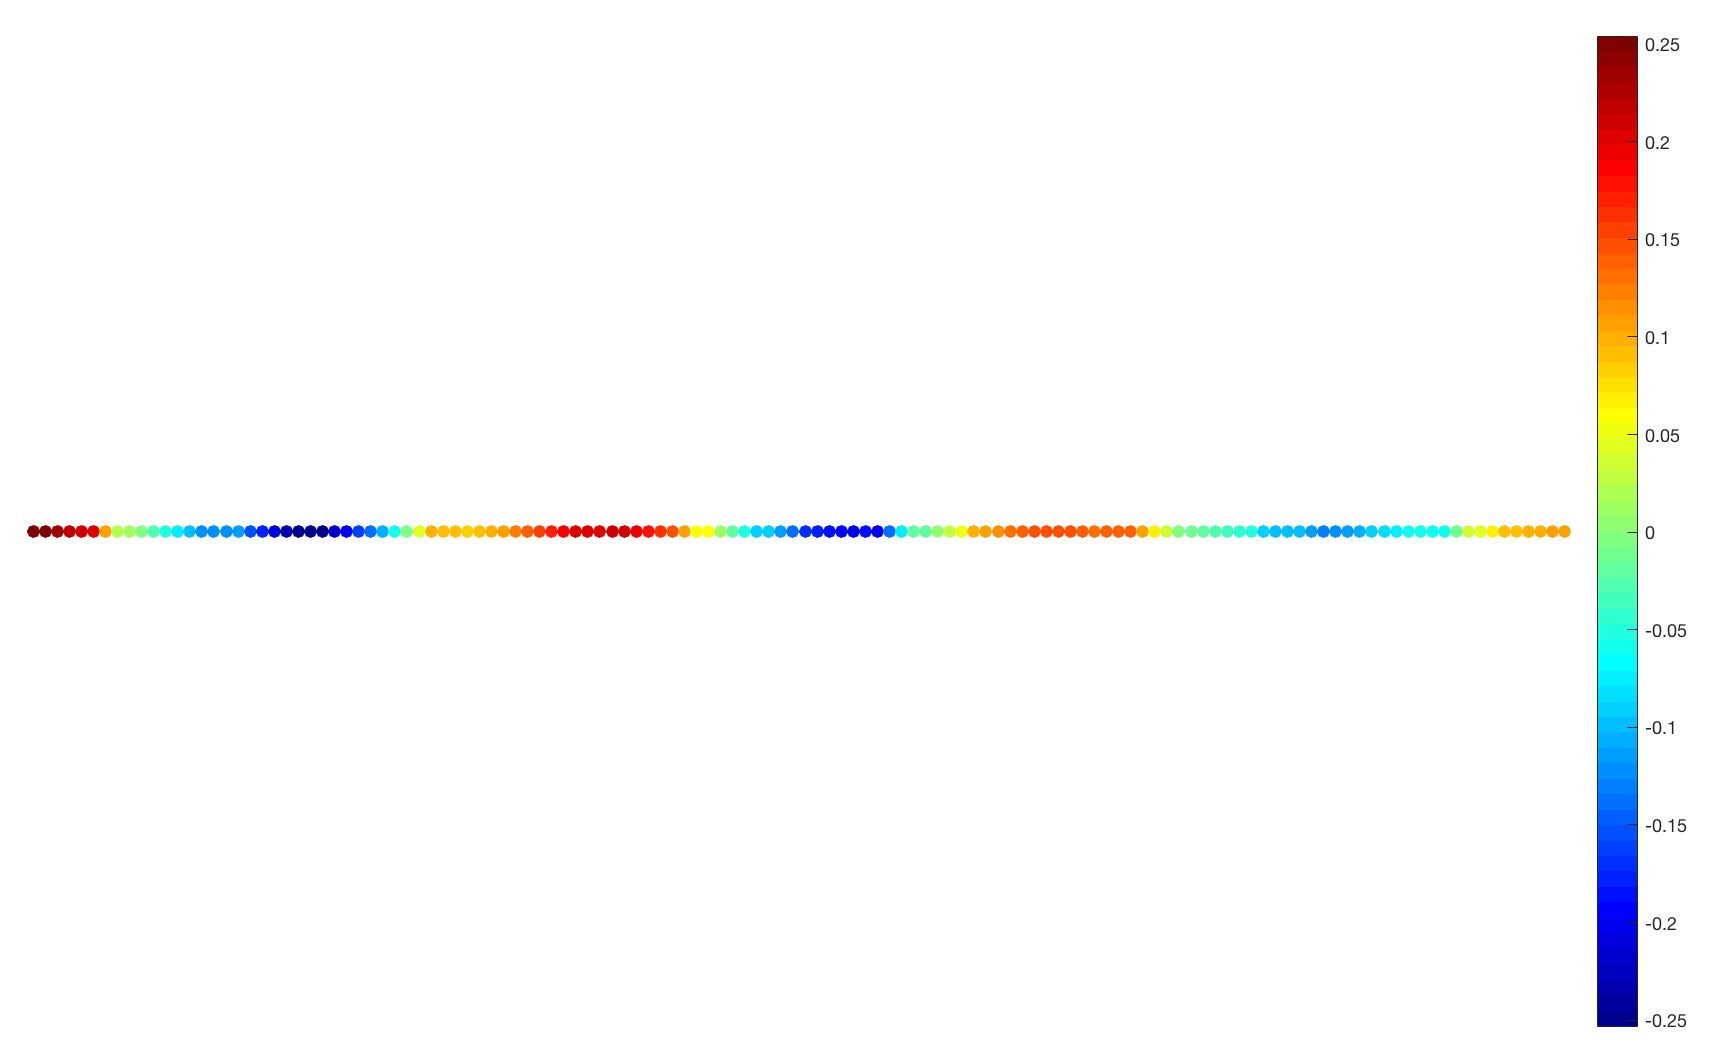
\includegraphics[width = 7 cm]{0629/path_graph_4_stages_7th_eigenvec_interpolated}
\caption{ (a) interpolation coefficient matrix (b) threshold at $x>10$ }
{(c) original 7th eigenvector (d) interpolated 7th eigenvector}
\end{figure}

The following images are produced under same process except the diagonals of Abars are kept non-zero at each stage.
\begin{figure}[H]
\centering
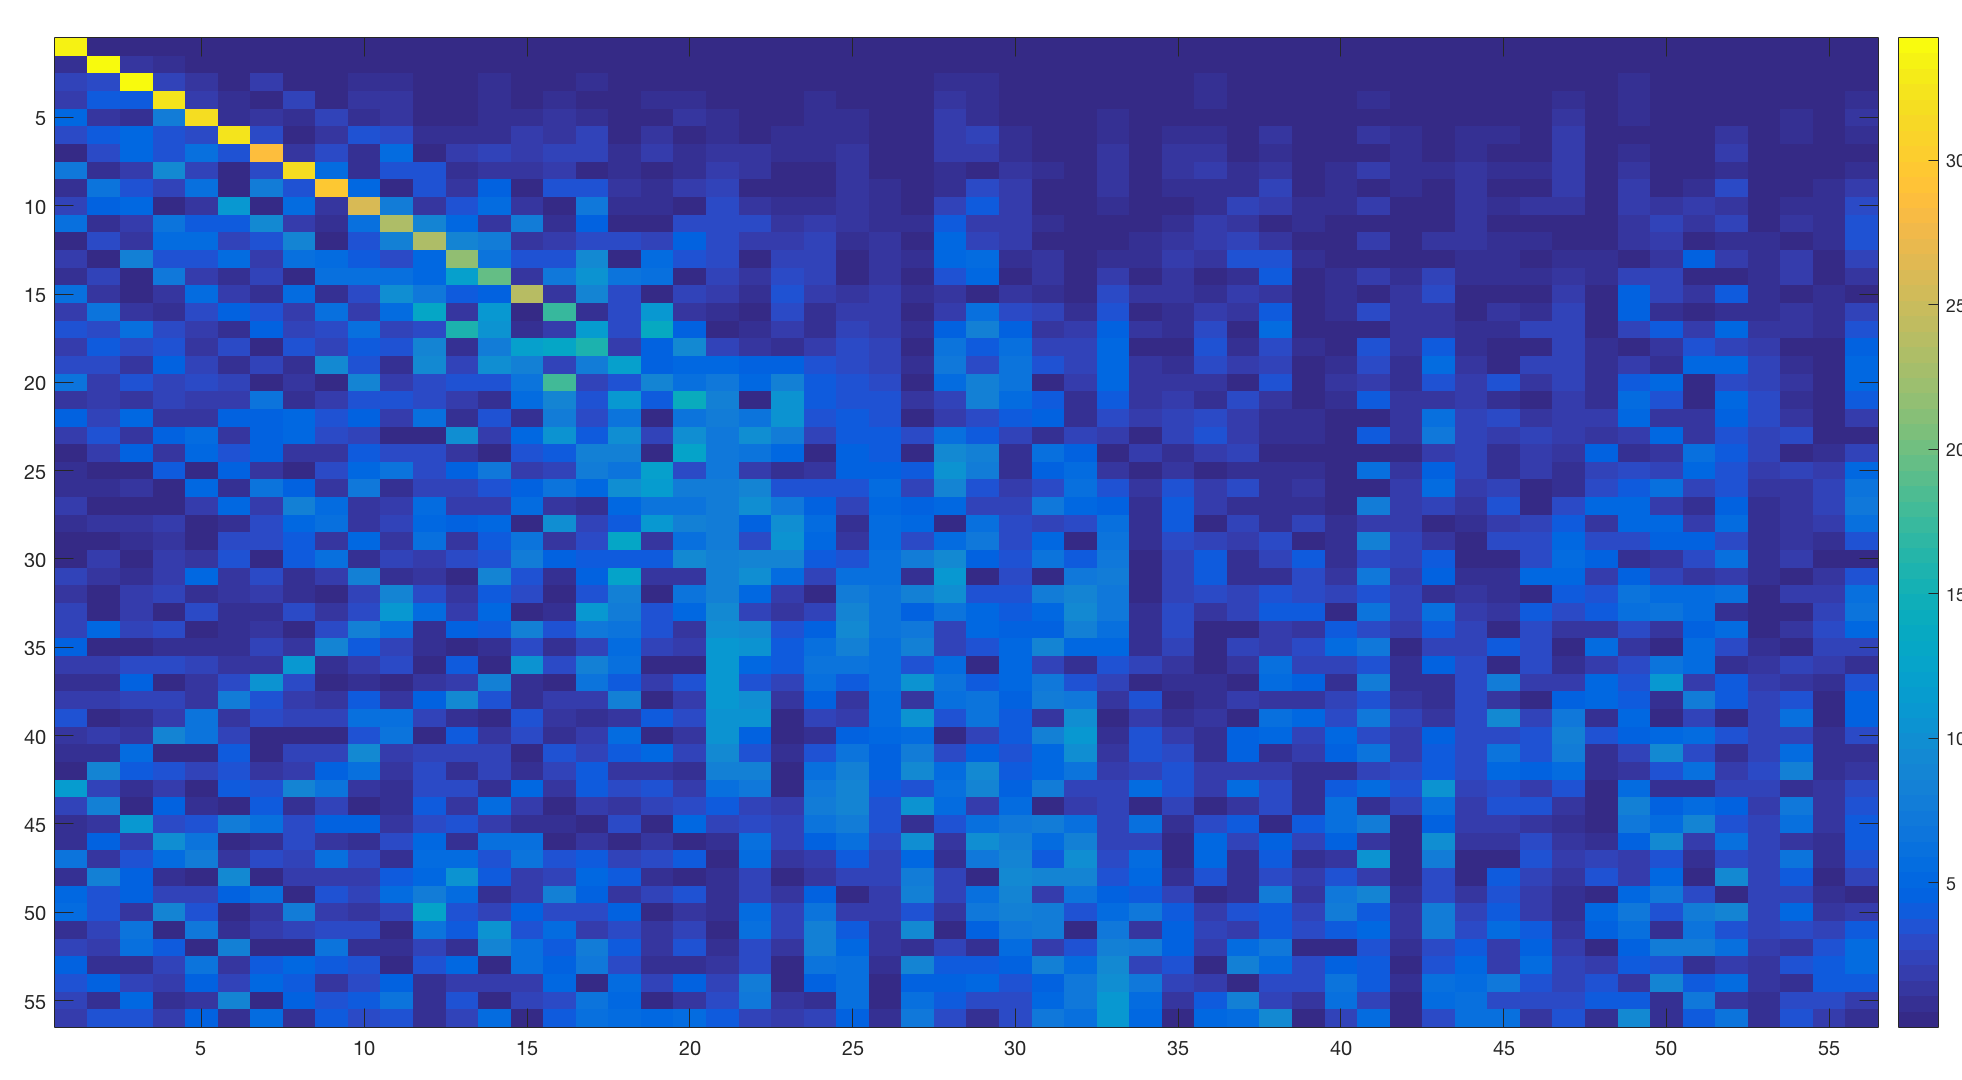
\includegraphics[width = 7 cm]{0629/original/coefficients_path_graph_4_stages}
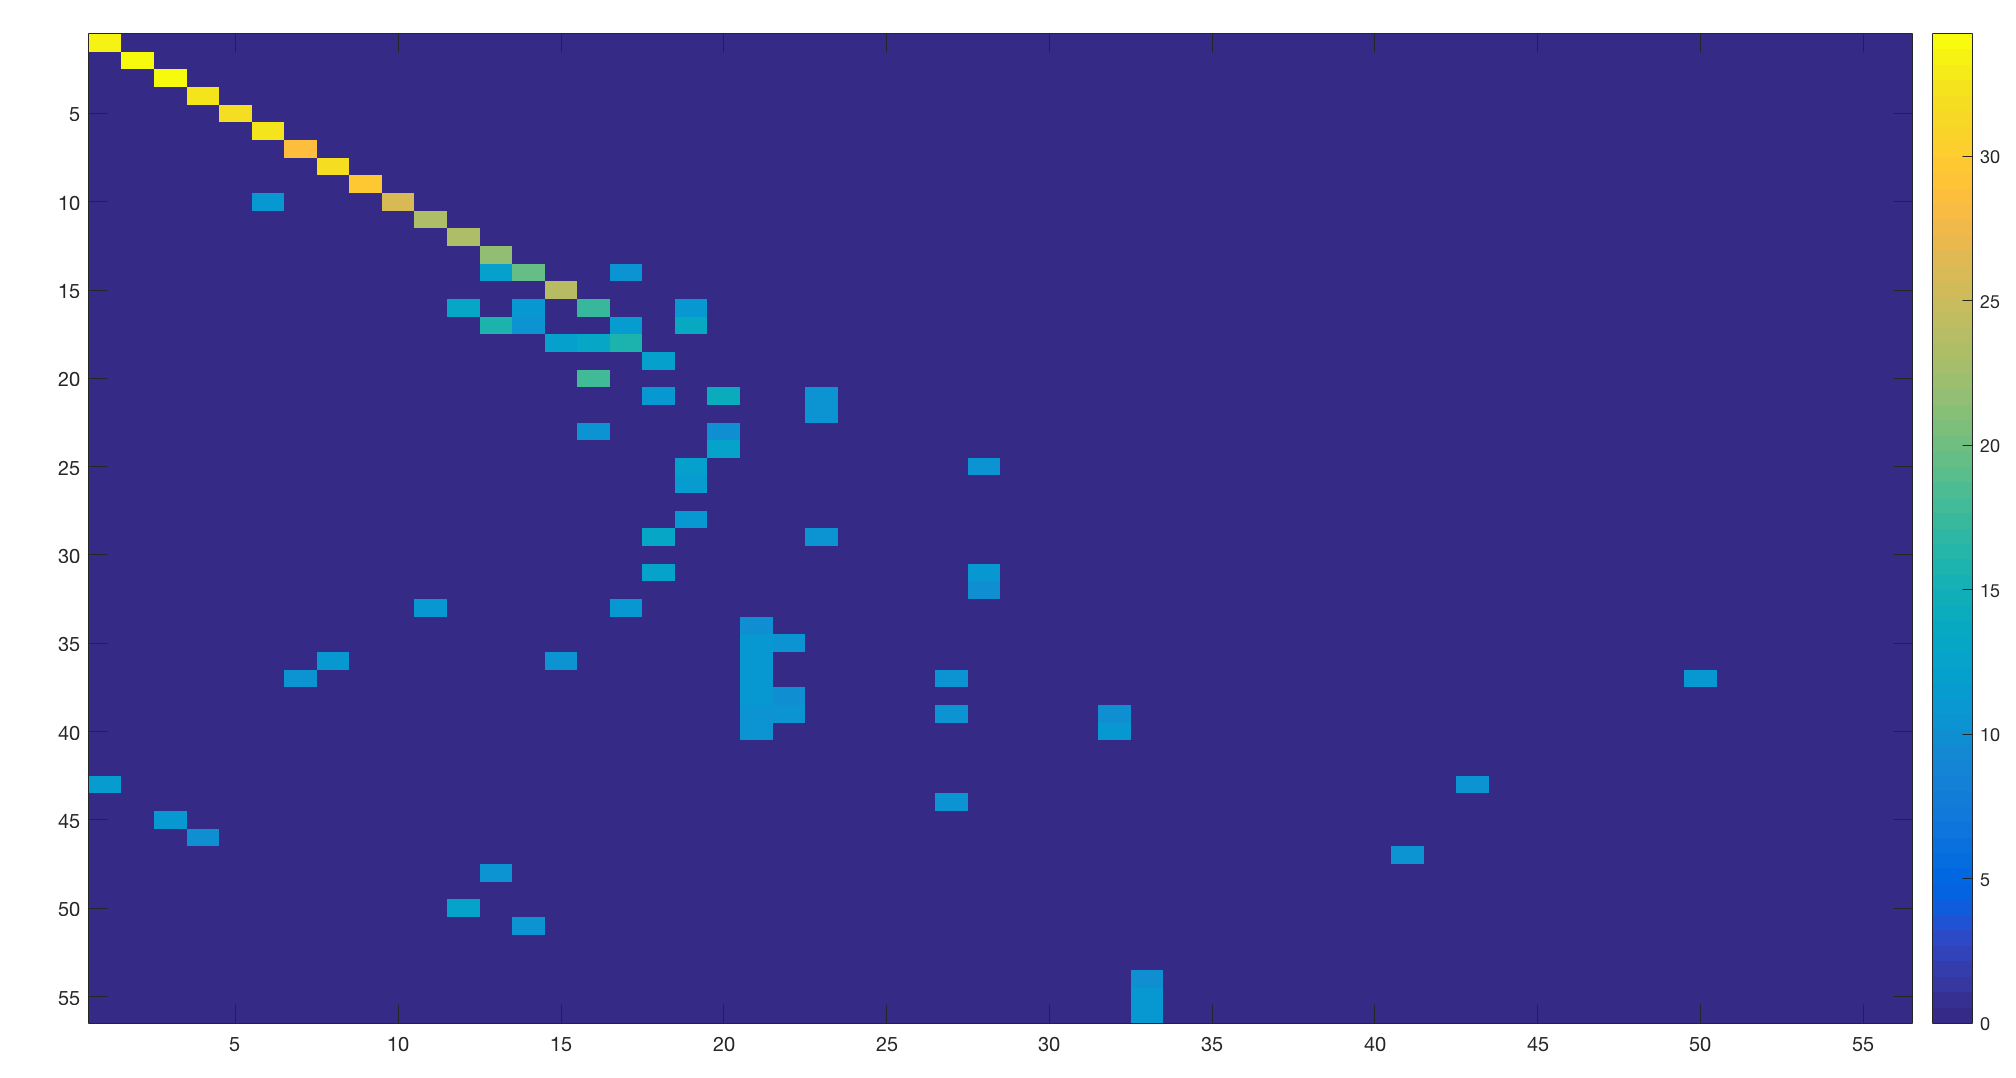
\includegraphics[width = 7 cm]{0629/original/coefficients_path_graph_4_stages_threshold}

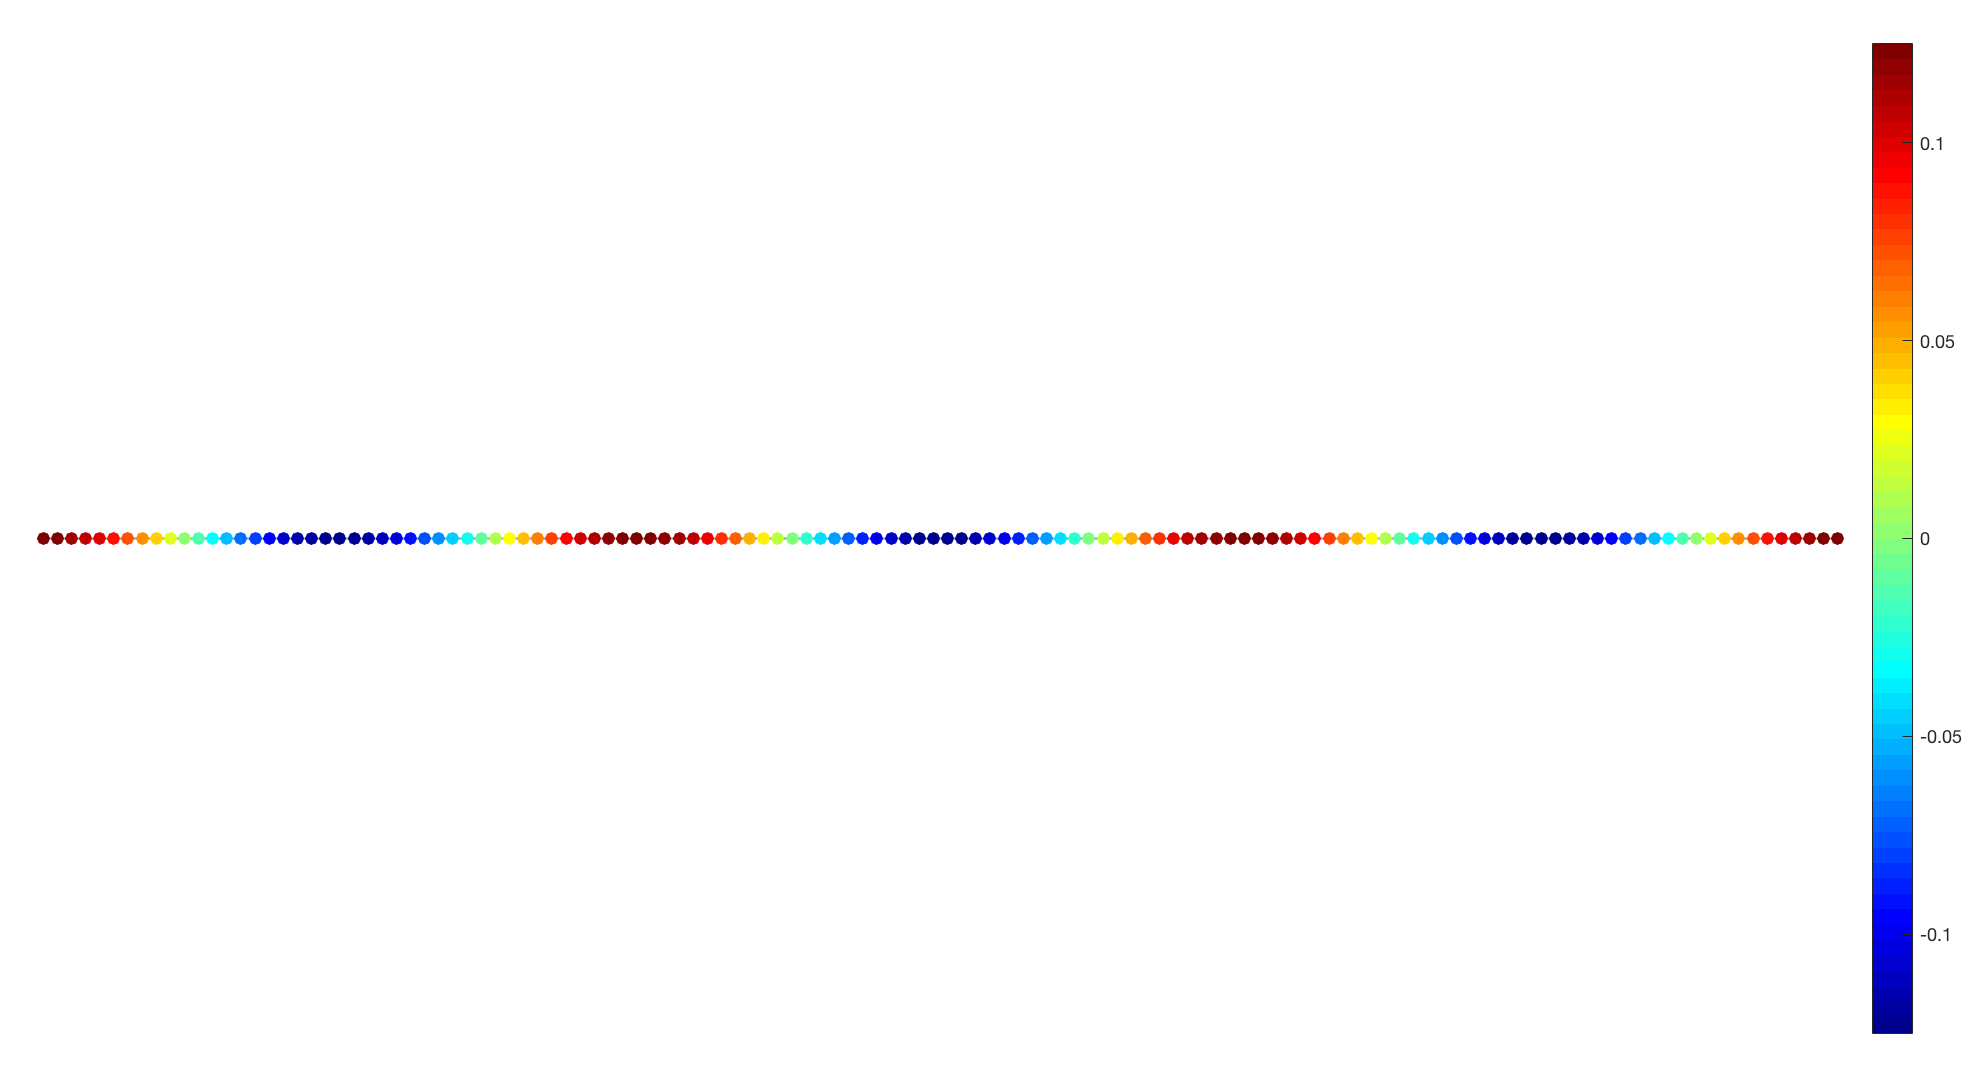
\includegraphics[width = 7cm]{0629/original/7th_eigen}
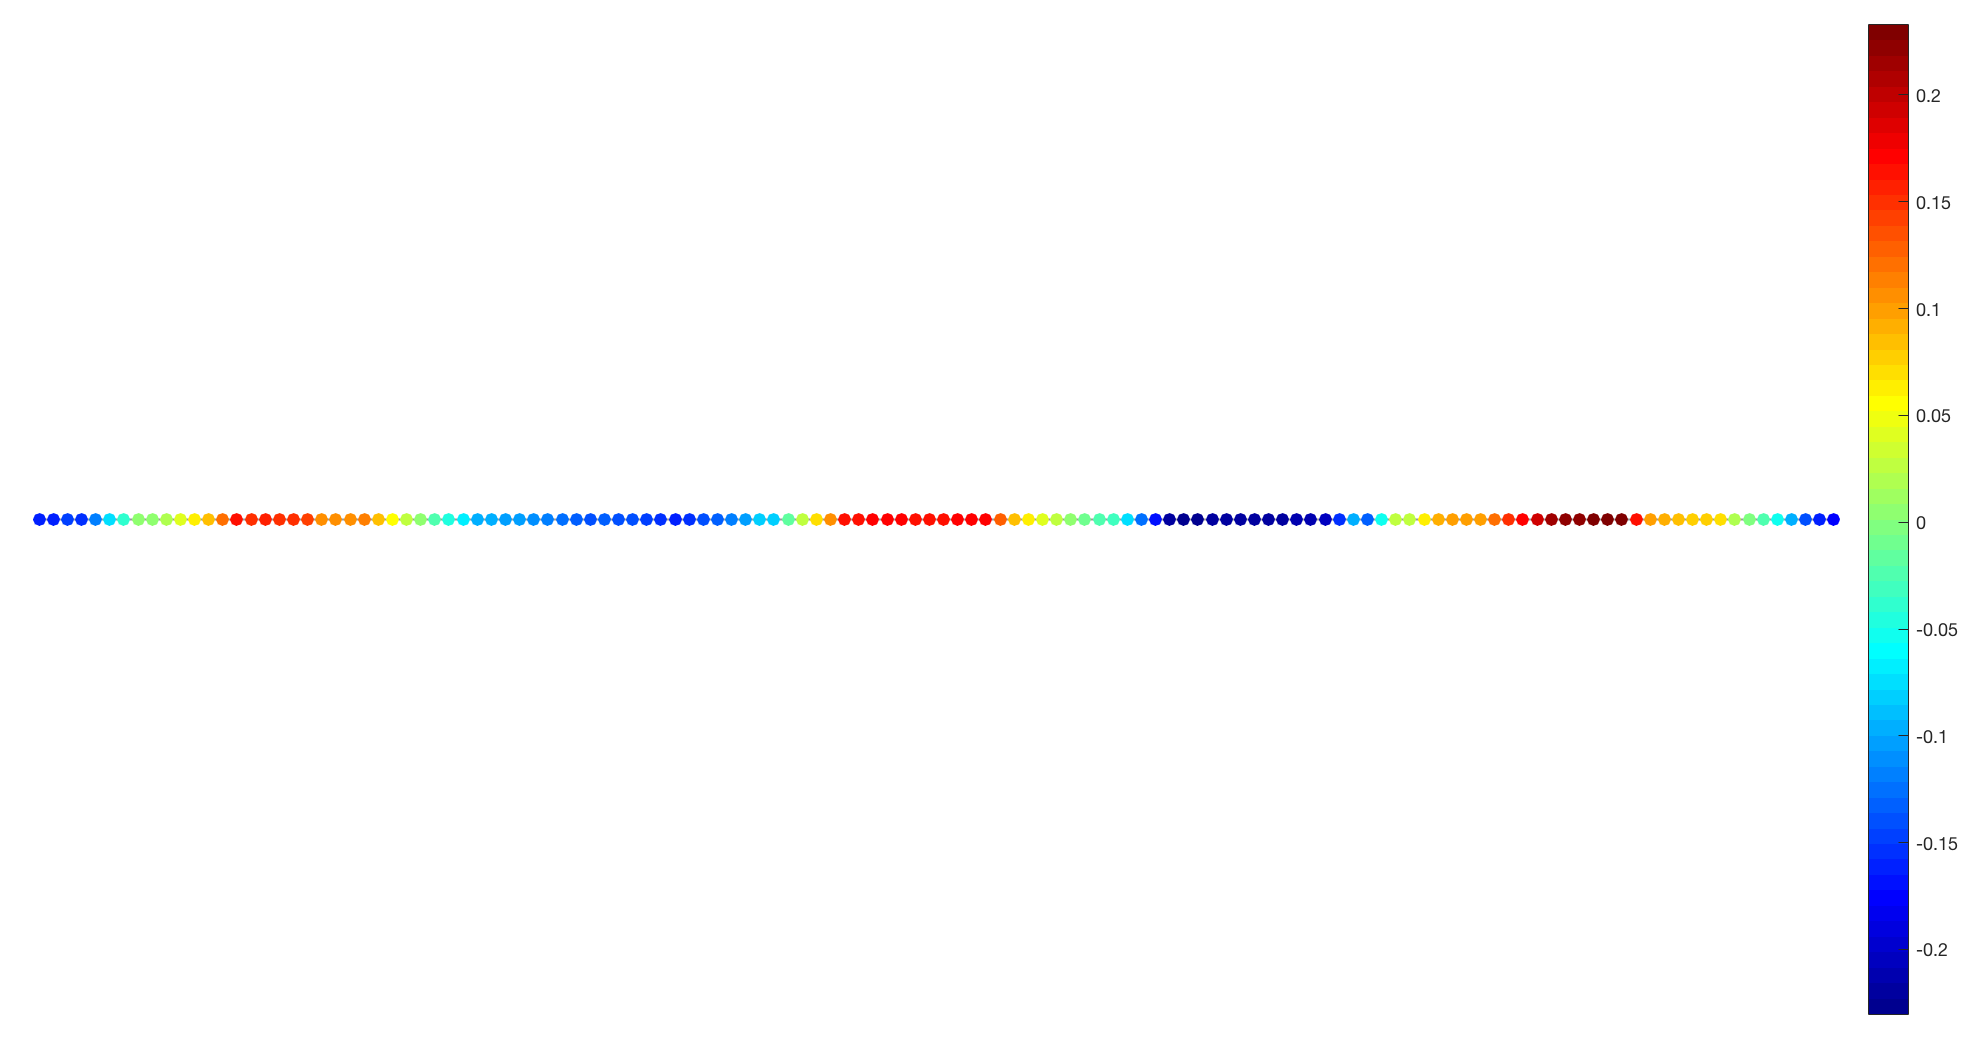
\includegraphics[width = 7 cm]{0629/original/7th_eigen_interpolated}
\caption{ (a) interpolation coefficient matrix (b) threshold at $x>10$ }
{(c) original 7th eigenvector (d) interpolated 7th eigenvector}
\end{figure}



The second example is on david\_sensor\_network graph. Parameters:
\begin{enumerate}
\item 500 vertices
\item compression ratio $\mu = 0.2$
\item 4 stages
\item 2 cluster
\end{enumerate}

\begin{figure}[H]
\centering
\includegraphics[width = 12 cm]{0629/graph}

\includegraphics[width = 12 cm]{0629/1st_downsampled}

\includegraphics[width = 12cm]{0629/2nd_downsampled}
\caption{ (a) original graph (b) 1st reduced graph (c) 2nd reduced graph}
\end{figure}


\begin{figure}[H]
\centering
\includegraphics[width = 12 cm]{0629/coefficients_zero_diagonal_4_stages}

\includegraphics[width = 12 cm]{0629/coefficients_zero_diagonal_4_stages_threshold}

\caption{ (a) interpolation coefficient matrix (b) threshold at $x>10$ }
\end{figure}

\newpage
\section{pMMF Multiresolution}
\subsection{pMMF Detailed Pseudocode}

\begin{algorithm}[H]
\caption{ComputeRotationMatrix}\label{givens}
\begin{algorithmic}[1]
\State \textbf{Input:} current cluster $A_1$, row/column indices $i$ and $j$, current Gram Matrix $G$

\State \textbf{set} $b = G(i, j)$
\State \textbf{set} $c = (G(j, j) - G(i, i))/2$;

\If {$g\neq 0$}
\State \textbf{set} $\beta = c / b$
\State \textbf{set} $tan(\alpha) = \frac{1}{|\beta| + \sqrt{\beta * \beta + 1}}$

\State \textbf{set}  $cos(\alpha) = \frac{1}{\sqrt{(t * t + 1)}}$;

\State \textbf{set}   $Q = \begin{bmatrix}
\cos(\alpha) & -\sin(\alpha) \\
\sin(\alpha)  & \cos(\alpha)
\end{bmatrix}$
\Else

$Q = I$
\EndIf
\State \textbf{Output:} $Q$
\end{algorithmic}
\end{algorithm}

Algorithm \ref{givens} finds an orthogonal rotation matrix $Q = \begin{bmatrix}
\cos(\alpha) & -\sin(\alpha) \\
\sin(\alpha)  & \cos(\alpha)
\end{bmatrix}$
 such that the second term of equation 20 is minimized when $k = 2$. That is to find an angle $\theta = 2\alpha$ such that $$\sin(\theta + \omega +\pi/2) = 0,, \text{where } \omega = \arctan(\frac{G(i,i) - G(j,j)}{2G(i,j)})$$
 
 Let $b = G(i, j)$ and $c = \frac{G(j, j) - G(i, i)}{2}$;
 
 Equivalently,
 $$\cos(\theta + \omega) = 0$$
 $$\theta = \pi/2-\omega = \pi/2 - \arctan(\frac{c}{b})$$
 
$$\tan(\alpha) = \tan(\theta/2) = \tan(\pi/4 - \frac{1}{2}\arctan(\frac{c}{b})) \text{     (if }\frac{c}{b}>0)$$
$$\tan(\alpha) = \frac{1}{\frac{c}{b} + \sqrt{(\frac{c}{b})^2 +1}}$$
$$\cos(\alpha) = \frac{1}{\sqrt{\tan(\alpha)^2 + 1}}$$
$$\sin(\alpha) = \tan(\alpha)*\sin(\alpha)$$

When $k>2$, the rotation matrix $Q$ is the eigenvectors of the $G_{I,I}$, where $I$ contains $k$ selected column indices. (why?)

Similarly, only the second term of equation 20 is minimized. That is,
$$\text{min } [QG_{I,I}Q^T]_{k,k}$$
Equivalently, $$\text{min } x^T[G_{I,I}]x \text{ such that } ||x||_2 = 1.$$
By Courant-Fischer theorem, $$\text{min } x^T[G_{I,I}]x = \lambda_1$$

Let $x$ be the smallest eigenvector $v_1$ of $G_{I,I}$. Then,
$$\text{min } x^T[G_{I,I}]x = \text{min } v_1^T[G_{I,I}]v_1 = v_1\lambda_1v_1 = \lambda_1$$


To find $k$ rows/columns involved in each rotation, pMMF uses the randomized greedy method. First, randomly select a column $i$, and then compute the inner product of this column with all other columns. The selected column set will include $k-1$ columns that have the largest inner products with column $i$. Algorithm 2 in ``Parallel MMF: a Multiresolution Approach to Matrix Computation'' gives a good description of this process.

Note that after we get the rotation matrix $Q$, we have to update the original matrix $A= QAQ^T$ and the Gram matrix $G = QGQ^T$ before next channel.

\begin{algorithm}[H]
\caption{pMMF}\label{pmmf}
\begin{algorithmic}[1]
\State \textbf{Input}: weighted adjacency matrix $A$, number of stages $P$, number of clusters $M$, compression ratio $\mu$, k-point rotation $k$

\medskip
\State \textbf{Set} the current active columns $A_0 = A$
\State \textbf{Set} the current column indices $orig\_idx{1} = 1:G.N$
\\ \quad\quad // $orig\_idx\{p+1\}$ keeps track of the columns indices at stage $p$ 

\State \textbf{Set} the current permutation $idx{1} = 1:G.N$
\\ \quad\quad // $idx\{p+1\}$ records the permutation applied to active columns at stage $p$ 

\medskip
\For{each stage $p = 1:P$}

\State \textbf{Cluster} the active columns into $M$ clusters;
\State \textbf{Set} $perm$ = permutation that will permute $A_{p-1}$ into correct cluster order
\State \textbf{Permute}  $A = A(perm, perm)$
\State \textbf{Update} $orig\_idx\{p+1\} = orig\_idx\{p\}(perm)$ 
\State \textbf{Update} $idx\{p+1\} = perm$

\medskip
\For{each cluster $m = 1:M$}
\State \textbf{Set} $Qs\{m\}$ = FindRotsInCluster(cluster, $\mu$, $k$, cInds)
\EndFor

\medskip
\State \textbf{Merge} $Qs$ together to get the rotation $Q\{p\}$ for stage $p$

\State \textbf{Update} $A = Q\{p\}AQ\{p\}^T$

\State \textbf{Set} $perm =$ permutation that puts active columns together
 
\State \textbf{Permute} $A = Q\{p\}AQ\{p\}^T$
\State \textbf{Update} $orig\_idx\{p+1\} = orig\_idx\{p+1\}(perm)$
\State \textbf{Update} $idx\{p+1\} = idx\{p+1\}(perm)$

\EndFor

\State \textbf{Output:} core $A$

\end{algorithmic}
\end{algorithm}

\subsection{Examples}

Now we construct a downsampled graph at each stage, taking the core to be a weighted adjacency matrix. Note that the core has non-zero diagonals. we simply set the diagonals to zero. \\
Parameters:
\begin{itemize}
\item $G$ = gsp\_david\_sensor\_network
\item 500 vertices
\item $A = G.W$
\item 4 stages
\item 2 clusters
\item 2-point rotations
\end{itemize}

\begin{figure}[H]
\centering
\includegraphics[width = 7cm]{multiresolution/multires1}
\includegraphics[width = 7cm]{multiresolution/multires2}

\includegraphics[width = 7cm]{multiresolution/multires3}
\includegraphics[width = 7cm]{multiresolution/multires4}

\includegraphics[width = 7cm]{multiresolution/multires5}

\caption{The top left figure is the original graph, gsp\_david\_sensor\_network with 500 vertices, and each subsequent figure is the result of one stage of downsampling.}
\end{figure}

\section{Double Procrustes Problem}

Double Procrustes problem considers finding an orthogonal matrix $Q$, which minimizes $$||Q^TAQ-B||$$ for symmetric $A$ and $B$. 

Since both $A$ and $B$ are symmetric, we can diagonalize these two matrices
$$ A = V_1D_1V_2^T\text{ and } B = V_2D_2V_2^T.$$
Then in this case, $Q = V_1 V_2^T$. (Detailed solution can be found in "Procrustes Problems", Oxford University Press). 

In the graph setting, we want to find an orthogonal $Q$, which minimizes $||Q^TLQ - L'||$, where $L$ is the original graph Laplacian and $L'$ is the reduced graph Laplacian. If we do multile levels, we could generate scaling and wavelet functions similar to pMMF. That is, the first $dim(V_L)$ rows of $Q$ are scaling functions and the rest of its rows are wavelets.

Some general observations;
\begin{enumerate}
\item This method connects Kron reduction and pMMF.
\item Q is not sparse.
\item The energy of scaling functions and wavelets are not localized.
\item Kron reduction produced dense sub-graphs.
\end{enumerate}

\section{Downsampling G.W}

The structure of the weighted adjacency matrix can be lost through downsampling -- we are often left with a core that has non-zero diagonal entries. We can maintain a zero diagonal, however, by being selective when we rotate columns within a certain cluster. If columns $i$ and $j$ only rotate with one another, and if $[A_{n-1}]_{i,i} = 0$, then $$[A_n]_{i,i} = [Q_nA_{n-1}Q_n^T]_{i,i} = 0$$ if vertices $i$ and $j$ are disconnected in the graph represented by the weighted adjacency matrix $A_{n-1}$:
\begin{align*}
[A_n]_{i,i} &= [Q_nA_{n-1}Q_n^T]_{i,i} \\
&= [Q_n]_{i,:}[A_{n-1}Q_n^T]_{:,i} \\
&= [Q_n]_{i,:}<[A_{n-1}]_{1,:}[Q_n^T]_{:,i} + \cdots + [A_{n-1}]_{s,:}[Q_n^T]_{:,i}> \\
&= [Q_n]_{i,1}[A_{n-1}]_{1,:}[Q_n^T]_{:,i} + \cdots + [Q_n]_{i,s}[A_{n-1}]_{s,:}[Q_n^T]_{:,i} 
\end{align*}
Since column $i$ only rotates with column $j$, the $i^{th}$ row of $Q_n$ will only have nonzero entries in the $i^{th}$ and $j^{th}$ columns. So, the above equation simplifies to
\begin{align*}
[A_n]_{i,i} &= [Q_n]_{i,i}[A_{n-1}]_{i,:}[Q_n^T]_{:,i} + [Q_n]_{i,j}[A_{n-1}]_{j,:}[Q_n^T]_{:,i}
\end{align*}
Likewise, the $i^{th}$ column of $Q_n^T$ will only have nonzero entries in the $i^{th}$ and $j^{th}$ rows. We now have
\begin{align*}
[A_n]_{i,i} &= [Q_n]_{i,i}([A_{n-1}]_{i,i}[Q_n^T]_{i,i} + [A_{n-1}]_{i,j}[Q_n^T]_{j,i}) + [Q_n]_{i,j}([A_{n-1}]_{j,i}[Q_n^T]_{i,i} + [A_{n-1}]_{j,j}[Q_n^T]_{j,i}) \\
&= [Q_n]_{i,i}(0 + [A_{n-1}]_{i,j}[Q_n^T]_{j,i}) + [Q_n]_{i,j}([A_{n-1}]_{j,i}[Q_n^T]_{i,i} + 0)
\end{align*} 
We have $[A_{n-1}]_{i,j} = [A_{n-1}]_{j,i}$ since $A$ is symmetric and $[Q_n]_{i,j} = [Q_n^T]_{j,i}$, so we are left with $$[A_n]_{i,i} = 2[A_{n-1}]_{i,j}[Q_n]_{i,i}[Q_n]_{i,j}$$
Since both entries of $Q_n$ are nonzero, $[A_n]_{i,i} = $ if and only if $[A_{n-1}]_{i,j} = 0$. \\
\\
The case is complicated further when, say, column $i$ rotates with both column $j$ and column $k$. Then, $Q_n$ has nonzero entries in the $i^{th}$, $j^{th}$, and $k^{th}$ columns, so we would end up with
\begin{align*}
[A_n]_{i,i} &= [Q_n]_{i,i}([A_{n-1}]_{i,i}[Q_n^T]_{i,i} + [A_{n-1}]_{i,j}[Q_n^T]_{j,i} + [A_{n-1}]_{i,k}[Q_n^T]_{k,i}) + [Q_n]_{i,j}([A_{n-1}]_{j,i}[Q_n^T]_{i,i} + [A_{n-1}]_{j,j}[Q_n^T]_{j,i}  \\
&+ [A_{n-1}]_{j,k}[Q_n^T]_{k,i}) + [Q_n]_{i,k}([A_{n-1}]_{k,i}[Q_n^T]_{i,i} + [A_{n-1}]_{k,j}[Q_n^T]_{j,i} + [A_{n-1}]_{k,k}[Q_n^T]_{k,i}) \\
&= 2[A_{n-1}]_{i,j}[Q_n]_{i,i}[Q_n]_{i,j} + 2[A_{n-1}]_{i,k}[Q_n]_{i,i}[Q_n]_{i,k} + 2[A_{n-1}]_{j,k}[Q_n]_{i,j}[Q_n]_{i,k}
\end{align*}
We see that $[A_{n-1}]_{j,k}$ now contributes as well. So, not only must the pairs $(i,j)$ and $(i,k)$ be disconnected, vertices $j$ and $k$ must also be disconnected even if they are not one of the pairs of columns that is rotated.\\
If we want to guarantee $[A_n]_{i,i} = 0$ for all $i$ in the cluster, the vertices in the cluster must all be mutually disconnected. However, this seems counterintuitive, since we normally would want to rotate similar vertices with one another. This method does the exact opposite, and as a result, downsampling results in edges between communities that were previously disconnected.

\begin{figure}[H]
\centering
\includegraphics[width = 7 cm]{disconnected_pMMF/discon_1}
\includegraphics[width = 7 cm]{disconnected_pMMF/discon_2}

\includegraphics[width = 7 cm]{disconnected_pMMF/discon_3}
\includegraphics[width = 7 cm]{disconnected_pMMF/discon_4}

\includegraphics[width = 7 cm]{disconnected_pMMF/discon_5}

\caption{pMMF performed on a 500 vertex sensor network with 4 stages, 4 clusters, 2-point rotations, and compression ratio 0.5. Rotations are performed only on disconnected vertices.}
\end{figure}

\section{Ron et al.}

Ron et al. assign a fraction $P_{ij}$ to a vertex's neighbors when it is eliminated. We combine this idea with pMMF. We use the downsampled graph generated by pMMF. If a givens rotation is performed between vertices $i$ and $j$ and $j$ is eliminated, the $P_{j, i} = 1$. The final reduced graph is $$W_{j,j'} = \sum P{mj} P{nj'} W_{mn}.$$

Reduced graphs:
\begin{figure}[H]
\centering
\includegraphics[width = 12 cm]{Ron_et_al/graph}

\includegraphics[width = 12 cm]{Ron_et_al/1st_reduced}

\includegraphics[width = 12 cm]{Ron_et_al/2nd_reduced}
\end{figure}

\section{Network Topology Identification from Spectral Templates}

Let the graph shift operator $S \in \R^{N\times N}$ be the adjacency matrix of a graph. Given the spectral templates $V = {v_1, \cdots, v_N}$, Segarra et al try to find
$$\text{min}_{S, \lambda} ||S||_0 $$
$$\text{subject to } S = V\lambda V^T $$
$$\text{and } \lambda_{1} =0, S_{i,j} \in [-1,0], S_{i,i} =1$$

Let $A$ be a heat diffusion on a given graph $G$, $A = G.Uf(G.e)G.U$. Perform pMMF on A and we get a core $H$. Our goal is to infer a graph structure based on $H$. Diagonalize $H = UVU^T$. We use U as our spectral templates. Our goal is to find

$$\text{min}_{S, \lambda} ||S||_0 $$
$$\text{subject to } S = V\lambda V^T $$
$$\text{and } \lambda_{1} =0, S_{i,j} \in [-1,0], S_{i,i} =1$$

\textbf{Relaxation:} $l_1$ norm penalized problem

$$\text{min}_{S, \lambda} \sum\sum W_{i,j}(p)|S_{i,j}| $$
$$\text{subject to } S = V\lambda V^T $$
$$\text{and } \lambda_{1} =0, S_{i,j} \in [-1,0], S_{i,i} =1$$

\begin{comment}
\section{Wiki Cartograph}
In Wiki Cartograph, each node represents a article and an directed edge $(i,j)$ exists when there is a link from article $i$ to article $j$.

We use a few different multiresolution methods on this graph: pMMF, pMMF combined with Ron et al and gsp\_multiresolutions.

\subsection{pMMF}

\subsection{pMMF with Ron et al}

\subsection{gsp\_multiresolutions}
\end{comment}





\end{document}